% =====================================================================
%  Chapter 1: Probability, Statistics, and the Language of Uncertainty
%  Source: Review.tex (Overleaf) + P1 transcription
% =====================================================================

\chapter{Probability, Statistics, and the Language of Uncertainty}
\label{chap_Review}

\section{A Paradigm Shift: From Classical to Frequentist to Bayesian}
\label{sec_paradigm}

``Probability approach in econometrics'' by Trygve \citet{Haavelmo1944} stands
at the beginning of a paradigm shift in statistical thinking; the
\emph{classical} interpretation of statistics is giving way to the
\emph{frequentist} interpretation. Under the classical interpretation,
probabilities are linked to the principle of indifference and statistical
events are governed by natural symmetry (e.g.\ coin tosses, die rolls).

Under the frequentist interpretation, probabilities of events are linked to
the frequency with which a given event is observed:
\begin{equation}
  P(x) = \lim_{n_t \to \infty} \frac{n_x}{n_t},
\end{equation}
where $n_x$ is the number of times event $x$ is observed and $n_t$ is the
total number of trials.

This probabilistic approach to statistics, which encompasses Bayesian
statistics\index{Bayesian statistics}, represents the world in terms of
``degrees of belief'' (Bayesian priors). More formally, \textbf{Bayes'
Theorem}\index{Bayes' Theorem} is expressed as the conditional probability of
event $A$ given $B$:

\begin{tcolorbox}[keyresult]
\begin{equation}
  P(A \mid B) = \frac{P(B \mid A)\,P(A)}{P(B)}
\end{equation}
\end{tcolorbox}


\section{Random Variables: Types and Typology}
\label{sec_RVtypes}

A random variable, usually written as $X$, is a variable whose possible values
are numerical outcomes of a random phenomenon. A random variable $X$ is a
(real) number with the following characteristics:

\begin{enumerate}[label=\alph*)]
  \item The value of $X$ is unknown.
  \item The possible values $X$ can take are known; the set of such values is
    called the \emph{support}, denoted $\boldsymbol{\mathcal{S}}_X$.
  \item If $\boldsymbol{\mathcal{A}} \subseteq \mathbb{R}$, we know the
    probability that $X$ belongs to $\boldsymbol{\mathcal{A}}$, denoted
    $P(X \in \boldsymbol{\mathcal{A}})$.
  \item If the value $x$ of $X$ becomes known such that $x=X$, then $x$ is
    called a \emph{realisation} of $X$.
\end{enumerate}

Random variables fall into two categories:

\begin{itemize}
  \item \textbf{Discrete random variables}\index{random variable!discrete}:
    Take only a countable number of distinct values (0, 1, 2, \ldots).
    Usually (but not necessarily) counts.
  \item \textbf{Continuous random variables}\index{random variable!continuous}:
    Take an infinite number of possible values. Usually measurements (height,
    weight, time).
\end{itemize}

We can also distinguish \emph{qualitative} (categorical) from
\emph{quantitative} variables:

\begin{itemize}
  \item \textbf{Nominal variables}\index{random variable!nominal}: Mutually
    exclusive, unordered categories (e.g.\ suburb type).
  \item \textbf{Ordinal variables}\index{random variable!ordinal}: Ordered
    categories where the differences between values are not meaningful (e.g.\
    quality-of-life rankings on a 1--10 scale).
  \item \textbf{Interval variables}\index{random variable!interval}:
    Differences are meaningful but there is no true zero (e.g.\ temperature
    in Celsius).
  \item \textbf{Ratio variables}\index{random variable!ratio}: A true zero
    exists and ratios are meaningful (e.g.\ height, weight, income).
\end{itemize}

\begin{table}[htp]
\centering
\caption{Basic statistical operations by variable type}
\label{tbl_Vars}
\renewcommand{\arraystretch}{1.3}
\begin{tabular}{@{}lcccc@{}}
\toprule
& \multicolumn{4}{c}{\emph{Variable type}} \\
\cmidrule{2-5}
\emph{Operation} & Nominal & Ordinal & Interval & Ratio \\
\midrule
Frequency distribution    & Yes & Yes & Yes & Yes \\
Median and percentiles    & No  & Yes & Yes & Yes \\
Addition / subtraction    & No  & No  & Yes & Yes \\
Mean, s.d., s.e.          & No  & No  & Yes & Yes \\
Ratio / coefficient of variation & No & No & No & Yes \\
\bottomrule
\end{tabular}
\renewcommand{\arraystretch}{1}
\end{table}


\section{Expectation and Variance}
\label{sec_Expectation}

\subsection{Expectation of a Discrete Random Variable}

\begin{equation}
  \E(X) = x_1 p_1 + x_2 p_2 + \cdots + x_n p_n = \sum_{i=1}^{n} x_i p_i
\end{equation}

In a finite sample, $\E(X)$ denotes the sample mean, and the sum of all
probabilities must equal one: $\sum_i p_i = 1$.

\paragraph{Example: The St.\ Petersburg Paradox}\index{St. Petersburg paradox}

Consider a gamble where an unbiased coin is tossed until tails ($T$) appears.
If $T$ shows up on the $n$-th toss, the payoff is $\$2^{n-1}$. How much would
you be willing to wager to participate?

\begin{align*}
  \E(X) &= \$2^0 \cdot \tfrac{1}{2} + \$2^1 \cdot \tfrac{1}{4}
           + \$2^2 \cdot \tfrac{1}{8} + \cdots \\
        &= \$1\cdot\tfrac{1}{2} + \$2\cdot\tfrac{1}{4}
           + \$4\cdot\tfrac{1}{8} + \cdots
         = \sum_{i=1}^{\infty} \$0.50 = \$\infty
\end{align*}

This is the St.~Petersburg Paradox, famously described by Daniel
Bernoulli\index{Bernoulli, Daniel} (1700--1782) to illustrate the failure of
the expected value principle in decision theory under uncertainty. The expected
payout is infinite, yet willingness to pay (WTP)\index{willingness to pay}
must be much less. The classical resolution introduces an explicit utility
function and the presumption of diminishing marginal utility, implying
$\E[U] < \E[X]$.

\paragraph{Example: Expected value of a pair of dice}

\begin{equation*}
  \E(X) = \tfrac{1}{6}\cdot1 + \tfrac{1}{6}\cdot2 + \cdots
          + \tfrac{1}{6}\cdot6 = 3.5
\end{equation*}

For a pair of dice, $\mu_X = 7$. Bivariate probabilities are shown in
Table~\ref{tbl_Dice}.

\begin{table}[htp]
\centering
\caption{Bivariate probabilities for a pair of dice}
\label{tbl_Dice}
\renewcommand{\arraystretch}{1.3}
\begin{tabular}{@{}lll|lll@{}}
\toprule
$X$ & $p$ & $Xp$ & $X$ & $p$ & $Xp$ \\
\midrule
$x_1$ & $p_1$ & $x_1p_1$ & 2  & 1/36 & 2/36  \\
$x_2$ & $p_2$ & $x_2p_2$ & 3  & 2/36 & 6/36  \\
      &       &           & 4  & 3/36 & 12/36 \\
      &       &           & 5  & 4/36 & 20/36 \\
      &       &           & 6  & 5/36 & 30/36 \\
      &       &           & 7  & 6/36 & 42/36 \\
      &       &           & 8  & 5/36 & 40/36 \\
      &       &           & 9  & 4/36 & 36/36 \\
      &       &           & 10 & 3/36 & 30/36 \\
      &       &           & 11 & 2/36 & 22/36 \\
$x_n$ & $p_n$ & $x_np_n$ & 12 & 1/36 & 6/36  \\
\midrule
\multicolumn{3}{l}{$\E(X)=\sum x_i p_i$} &&
\multicolumn{2}{r}{252/36 = 7} \\
\bottomrule
\end{tabular}
\renewcommand{\arraystretch}{1}
\end{table}

\subsection{Expectation Rules}

\begin{enumerate}
  \item $\E[X + Y + Z] = \E[X] + \E[Y] + \E[Z]$
  \item $\E[bX] = b\E[X]$
  \item $\E[b] = b$
  \item $\E[a + bX] = a + b\E[X]$
\end{enumerate}

\paragraph{Example} Let $V \sim \mathcal{N}(0,1)$ and $Z \equiv \mu + \sigma V$.
Then $\E[Z] = \mu$ and $\Var[Z] = \sigma^2$, since $\E[V]=0$ and
$\E[V^2]=1$.

\subsection{Variance}

\begin{equation}
  \Var(X) = \sigma^2_X = \E\bigl[(X-\mu_X)^2\bigr]
  = \sum_{i=1}^{n}(x_i - \mu_X)^2 p_i
\end{equation}

Alternative expression (computing formula):
\begin{align}
  \Var(X) &= \E\bigl[X^2 - 2\mu_X X + \mu_X^2\bigr] \nonumber \\
          &= \E[X^2] - 2\mu_X \E[X] + \mu_X^2 \nonumber \\
          &= \E[X^2] - \mu_X^2
\end{align}

\subsection{Fixed and Random Decomposition of Variables}

Let the random variable $X$ be decomposed into a constant mean $\mu_X$ and a
stochastic disturbance term $u$:
\begin{equation}
  X = \mu_X + u, \qquad \E[u] = \E[X - \mu_X] = 0
\end{equation}
Since all variation in $X$ is due to $u$, the variance of $X$ equals the
variance of the disturbance:
\begin{equation}
  \sigma^2_X = \E[(X-\mu_X)^2] = \E[u^2] = \sigma^2_u
\end{equation}
This decomposition into a \emph{systematic} (fixed) component and a
\emph{stochastic} (random) component is the conceptual foundation of every
regression model in this book.


\section{Continuous Random Variables}
\label{sec_ContRV}

All random variables have a \textbf{probability density function}
(PDF)\index{density function!probability} and a \textbf{cumulative density
function} (CDF)\index{density function!cumulative}:
\begin{equation}
  \Pr[A \leq x \leq B] = \int_A^B f(x)\,dx, \qquad
  F(x) = \int_{-\infty}^{x} f(t)\,dt = F(B) - F(A)
\end{equation}

The expectation and variance of a continuous random variable:
\begin{equation}
  \E[X] = \int_{-\infty}^{\infty} x\,f(x)\,dx = \mu_x,
  \qquad
  \Var(X) = \int_{-\infty}^{\infty}(x - \mu_x)^2 f(x)\,dx = \sigma_x^2
\end{equation}

\begin{figure}[htp]
\centering
\begin{tikzpicture}[>=Stealth, scale=1.1]
  % Left panel: PDF
  \begin{scope}[xshift=0cm]
    \draw[->] (-2.5,0) -- (2.7,0) node[right] {$x$};
    \draw[->] (0,-0.1) -- (0,1.6) node[above] {$f(x)$};
    \draw[very thick, domain=-2.4:2.4, samples=80]
      plot (\x, {1.3*exp(-0.8*\x*\x)});
    % Shaded region between -1.5 and -0.5
    \fill[gray!30, domain=-1.5:-0.5, samples=40]
      (-1.5,0) -- plot (\x, {1.3*exp(-0.8*\x*\x)}) -- (-0.5,0) -- cycle;
    \draw[dashed] (-1.5,0) node[below]{\small$A$}
                         -- (-1.5, {1.3*exp(-0.8*1.5*1.5)});
    \draw[dashed] (-0.5,0) node[below]{\small$B$}
                         -- (-0.5, {1.3*exp(-0.8*0.5*0.5)});
    \node[below=18pt] at (0,0) {PDF:\; $f(x) \equiv F'(x)$};
  \end{scope}
  % Right panel: CDF
  \begin{scope}[xshift=6cm]
    \draw[->] (-2.5,0) -- (2.7,0) node[right] {$x$};
    \draw[->] (0,-0.1) -- (0,1.6) node[above] {$F(x)$};
    \draw[very thick, domain=-2.4:2.4, samples=80]
      plot (\x, {1.3/(1+exp(-2.2*\x))});
    \draw[dashed] (-1.5,0) node[below]{\small$A$}
                         -- (-1.5, {1.3/(1+exp(2.2*1.5))});
    \draw[dashed] (-0.5,0) node[below]{\small$B$}
                         -- (-0.5, {1.3/(1+exp(2.2*0.5))});
    \node[below=18pt] at (0,0) {CDF:\; $F(x) = \int_{-\infty}^x f(t)\,dt$};
  \end{scope}
\end{tikzpicture}
\caption{Probability density function (PDF) and cumulative density function
(CDF) for a continuous random variable. The shaded area in the PDF equals
$\Pr[A \leq x \leq B]$.}
\label{fig_PDFCDF}
\end{figure}


\section{Moments: Skewness and Kurtosis}
\label{sec_Moments}

Higher-order moments describe the shape of a distribution beyond its mean and
variance.

\noindent\textbf{Skewness} ($3$rd central moment / $\sigma^3$):
\begin{equation}
  \gamma_1 = \frac{\E[(X-\mu)^3]}{\sigma^3}
  \qquad
  \begin{cases} > 0 & \text{right-skewed (positive tail)} \\
                = 0 & \text{symmetric} \\
                < 0 & \text{left-skewed (negative tail)}
  \end{cases}
\end{equation}

\noindent\textbf{Kurtosis} ($4$th central moment / $\sigma^4$):
\begin{equation}
  \gamma_2 = \frac{\E[(X-\mu)^4]}{\sigma^4}
  \qquad
  \begin{cases} > 3 & \text{leptokurtic (fat tails)} \\
                = 3 & \text{mesokurtic (normal)} \\
                < 3 & \text{platykurtic (thin tails)}
  \end{cases}
\end{equation}


\section{Covariance, Correlation, and Joint Distributions}
\label{sec_CovCorr}

\begin{equation}
  \Cov(X,Y) = \sigma_{XY} = \E[(X-\mu_X)(Y-\mu_Y)]
             = \E[XY] - \mu_X\mu_Y
\end{equation}

\begin{equation}
  \rho_{XY} = \frac{\Cov(X,Y)}{\sigma_X \sigma_Y} \;\in\; [-1,+1]
\end{equation}

\noindent\textbf{Covariance and correlation rules:}
\begin{enumerate}[label=(\roman*)]
  \item $\Cov(X,X) = \Var(X)$
  \item $\Cov(aX,bY) = ab\,\Cov(X,Y)$
  \item $\Var(X+Y) = \Var(X) + \Var(Y) + 2\Cov(X,Y)$
  \item If $X \ind Y$: $\Cov(X,Y) = 0$ and $\Var(X+Y) = \Var(X)+\Var(Y)$
\end{enumerate}

\noindent\textbf{Sample estimators:}
\begin{equation}
  \hat{\sigma}_{XY} = \frac{1}{n-1}\sum_{i=1}^{n}(x_i-\bar{x})(y_i-\bar{y}),
  \qquad
  \hat{\rho}_{XY} = \frac{\hat{\sigma}_{XY}}{\hat{\sigma}_X\hat{\sigma}_Y}
\end{equation}


\section{Estimator Properties}
\label{sec_EstimatorProps}

Let $\hat{\theta}$ be an estimator of population parameter $\theta$.

\subsection{Unbiasedness}

$\hat{\theta}$ is \textbf{unbiased} if $\E[\hat{\theta}] = \theta$.
The \textbf{bias} is $\text{Bias}(\hat{\theta}) = \E[\hat{\theta}] - \theta$.

\subsection{Efficiency}

Among all unbiased estimators, $\hat{\theta}$ is \textbf{efficient} (best) if
it has the smallest variance. The Cramér-Rao lower bound defines the minimum
variance achievable by an unbiased estimator.

\begin{figure}[htp]
\centering
\begin{tikzpicture}[>=Stealth, scale=1.0]
  % Efficient estimator (narrow)
  \draw[very thick, domain=-2:2, samples=60]
    plot (\x, {1.8*exp(-3*\x*\x)}) node[right]{\small Efficient $\hat\theta_1$};
  % Inefficient estimator (wide)
  \draw[thick, dashed, domain=-3.5:3.5, samples=80]
    plot (\x, {0.9*exp(-0.6*\x*\x)}) node[right]{\small Inefficient $\hat\theta_2$};
  % True value
  \draw[gray, thin] (0,-0.1) -- (0,1.95);
  \node[below] at (0,-0.1) {$\theta$};
  \draw[->] (-3.8,0) -- (4.2,0) node[right] {$\hat\theta$};
  \draw[->] (0,-0.15) -- (0,2.2);
\end{tikzpicture}
\caption{Efficiency: $\hat\theta_1$ is more efficient than $\hat\theta_2$
because it has smaller variance around the true parameter value $\theta$.}
\label{fig_Efficiency}
\end{figure}

\subsection{Mean Squared Error}

\begin{tcolorbox}[keyresult]
\begin{equation}
  \MSE(\hat{\theta}) = \E[(\hat{\theta} - \theta)^2]
  = \Var(\hat{\theta}) + \bigl[\text{Bias}(\hat{\theta})\bigr]^2
\end{equation}
\end{tcolorbox}

This decomposition shows the fundamental bias--variance trade-off: a slightly
biased estimator may have lower MSE than an unbiased one if its variance is
sufficiently smaller.

\subsection{Consistency}

$\hat{\theta}_n$ is \textbf{consistent} if $\hat{\theta}_n
\xrightarrow{p} \theta$ as $n \to \infty$:
\begin{equation}
  \lim_{n \to \infty} P(|\hat{\theta}_n - \theta| > \varepsilon) = 0
  \quad \forall\,\varepsilon > 0
\end{equation}

\begin{figure}[htp]
\centering
\begin{tikzpicture}[>=Stealth, scale=0.95]
  \def\tp{0}  % true parameter
  \foreach \s/\lbl in {1.2/{$n=10$}, 0.7/{$n=50$}, 0.3/{$n=200$}}{
    \draw[domain={\tp-3.5*\s}:{\tp+3.5*\s}, samples=60, thick]
      plot (\x, {1/(\s*sqrt(2*3.14159))*exp(-0.5*((\x-\tp)/\s)^2)});
  }
  \draw[->] (-4.2,0) -- (4.2,0) node[right]{$\hat\theta$};
  \draw[->] (0,-0.1) -- (0,1.5);
  \draw[gray, thin] (\tp,-0.05) -- (\tp,1.45);
  \node[below] at (\tp,-0.05) {$\theta$};
  \node[right] at (1.5,1.3) {\small $n=200$};
  \node[right] at (1.8,0.55) {\small $n=50$};
  \node[right] at (2.5,0.28) {\small $n=10$};
\end{tikzpicture}
\caption{Consistency: as $n$ increases, the sampling distribution of
$\hat\theta$ shrinks around the true value $\theta$.}
\label{fig_Consistency}
\end{figure}


\section{Statistical Inference}
\label{sec_Inference}

\subsection{The Hypothesis Testing Framework}

\begin{enumerate}
  \item Formulate $H_0$ (null) and $H_1$ (alternative)
  \item Choose significance level $\alpha$ (typically 0.01, 0.05, 0.10)
  \item Compute test statistic and $p$-value
  \item Reject $H_0$ if $p < \alpha$
\end{enumerate}

\begin{table}[htp]
\centering
\caption{Decision outcomes in hypothesis testing}
\label{tbl_TypeErrors}
\renewcommand{\arraystretch}{1.3}
\begin{tabular}{@{}lcc@{}}
\toprule
& $H_0$ True & $H_0$ False \\
\midrule
Fail to reject $H_0$ & Correct ($1-\alpha$) & Type II error ($\beta$) \\
Reject $H_0$         & Type I error ($\alpha$) & Correct ($1-\beta$) \\
\bottomrule
\end{tabular}
\renewcommand{\arraystretch}{1}
\end{table}

\subsection{The $z$-Statistic and $p$-Values}

For a test of $H_0: \mu = \mu_0$:
\begin{equation}
  z = \frac{\bar{x} - \mu_0}{\sigma/\sqrt{n}}
  \sim \mathcal{N}(0,1) \quad \text{under } H_0
\end{equation}

\begin{tcolorbox}[keyresult]
Two-sided $p$-value:\quad $p(\hat{z}) = 2\bigl(1 - \Phi(|\hat{z}|)\bigr)$
\end{tcolorbox}

\subsection{Statistical Power}

The \textbf{power} of a test is $1 - \beta$, the probability of correctly
rejecting a false null hypothesis.

\begin{figure}[htp]
\centering
\begin{tikzpicture}[>=Stealth, scale=1.0]
  % H0 distribution (centred at 0)
  \draw[very thick, domain=-3:3, samples=80]
    plot (\x, {1.2*exp(-0.8*\x*\x)});
  \node at (-1.8, 0.9) {$H_0$};
  % H1 distribution (centred at 2)
  \draw[very thick, dashed, domain=-1:5, samples=80]
    plot (\x, {1.2*exp(-0.8*(\x-2)*(\x-2))});
  \node at (3.8, 0.9) {$H_1$};
  % Critical value
  \draw[gray, thin] (1.4,-0.05) -- (1.4,1.3);
  \node[below] at (1.4,-0.05) {\small $z_\alpha$};
  % Type II error region (shaded)
  \fill[gray!30, domain=-1:1.4, samples=40]
    (-1,0) -- plot (\x, {1.2*exp(-0.8*(\x-2)*(\x-2))}) -- (1.4,0) -- cycle;
  \node at (0.2, 0.18) {\small $\beta$};
  % Rejection region label
  \node at (2.5, 0.2) {\small Power $= 1-\beta$};
  \draw[->] (-3.5,0) -- (5.5,0) node[right]{$z$};
  \draw[->] (0,-0.1) -- (0,1.5);
\end{tikzpicture}
\caption{Statistical power. The shaded region represents the Type II error
probability $\beta$; power is $1-\beta$.}
\label{fig_Power}
\end{figure}

\subsection{Confidence Intervals}

A $(1-\alpha)\times100\%$ confidence interval for $\mu$:
\begin{equation}
  \bar{x} \pm z_{\alpha/2}\,\frac{\sigma}{\sqrt{n}}
\end{equation}

With unknown $\sigma$, replace $z_{\alpha/2}$ with $t_{\alpha/2, n-1}$.
The \textbf{$t$-distribution}\index{t-distribution} with $\nu$ degrees of
freedom has heavier tails than the standard normal and converges to
$\mathcal{N}(0,1)$ as $\nu \to \infty$.

\subsection{Probability Limits and Asymptotic Theory}

The \textbf{probability limit}\index{probability limit} ($\plim$) satisfies
the following rules:

\begin{enumerate}[label=(\roman*)]
  \item $\plim(X + Y) = \plim(X) + \plim(Y)$
  \item $\plim(XY) = \plim(X)\cdot\plim(Y)$
  \item $\plim(X/Y) = \plim(X)/\plim(Y)$ \;(if $\plim(Y) \neq 0$)
  \item $\plim[g(X)] = g(\plim X)$ \;(continuous $g$; Slutsky's theorem)
  \item $\plim(\bar{X}) = \mu$ \;(law of large numbers)
  \item $\plim(\hat{\sigma}^2) = \sigma^2$ \;(consistency of sample variance)
\end{enumerate}


\section{The Central Limit Theorem}
\label{sec_CLT}

\subsection{Lindberg-Lévy CLT}

For i.i.d.\ random variables $x_t$ with mean $\mu$ and variance $\sigma^2$,
the \textbf{Central Limit Theorem}\index{central limit theorem} (CLT) states
that:

\begin{tcolorbox}[keyresult]
\begin{equation}
  z_t \equiv \frac{1}{\sqrt{n}}\sum_{t=1}^{n}\frac{x_t - \mu}{\sigma}
  \xrightarrow{d} \mathcal{N}(0,1) \quad \text{as } n \to \infty
  \label{eqn_CLT}
\end{equation}
\end{tcolorbox}

\subsection{CLT in Practice: How Large Does $n$ Need to Be?}

The CLT becomes effective at surprisingly small $n$ for many distributions:

\begin{itemize}
  \item \textbf{Binomial:} Approximation improves dramatically at $n=50$.
  \item \textbf{Exponential:} CLT takes effect visibly at $n=50$.
  \item \textbf{$t$-distribution:} Even at $n=10$, centered random variables
    approximate $\mathcal{N}(0,1)$ well (the two distributions are similar
    except for heavier tails in the $t$).
  \item \textbf{Gamma/Beta:} Reasonable approximation at smallest $n$,
    reliable at $n=50$.
  \item \textbf{Log-normal:} CLT kicks in only at $n > 100$ due to high skew.
\end{itemize}

\noindent\textbf{Variance and sample size as substitutes.} The $\chi^2(m)$
distribution approaches $\mathcal{N}(m, 2m)$ as $m$ becomes large. A higher
variance implies a larger denominator in the centering process, which in turn
requires \emph{fewer} observations for the distribution to be approximately
standard normal. Variance and sample size are substitutes in the centering
process.

\renewcommand\bibname{Further reading}
\begin{subappendices}
\bibliographystyle{econometrica}
\bibliography{Literature/OverLord}
\IfFileExists{Literature/Review.bbl}{\chapter{Review}\label{chap_Review}
\section{Preliminaries}\label{chap_Review:Prelim}
``Probability approach in econometrics'' by Trygve \citet{Haavelmo1944} stands at the beginning of a paradigm shift in statistical thinking; the \emph{classical} interpretation of statistics is giving way to the \emph{frequentist} interpretation. Under the classical interpretation, probabilities are linked to the principle of indifference and statistical events are governed by natural symmetry (e.g. coin tosses, die etc.) This constraining set-up of what gives rise to probabilities is one of the key problems of the classical view. 

Under the frequentist interpretation on the other hand, probabilities of events are linked to the frequency with which a given event is observed. This implies that

$$P(x)= \lim\limits_{n_{t} \rightarrow \infty} \frac{n_{x}}{n_{t}},$$ 

where $n_{x}$ is the number of observed trials and $n_{t}$ is the total number of trials. This probabilistic approach to statistics, which includes Bayesian statistics\index{Bayesian statistics}, represents the world in terms of ``degrees of belief'' (Bayesian priors).

More formally, Bayes' Theorem is expressed as the conditional probability of occurence A given B such that $$P(A|B) = \frac{P(B|A)P(A)}{P(B)}.$$\index{Bayes' Theorem|see{Bayesian statistics}}


\section{Statistics and probability theory}\label{chap_Review:Stats}
\subsection{Types of random variables}
A random variable, usually written as $X$, is a variable whose possible values are numerical outcomes of a random phenomenon. A random variable $X$  is a (real) number with the following characteristics:

\begin{inparaenum}[\itshape a\upshape)]
\item the value of $X$ is unknown;
\item the possible values $X$ can take are known; the set of such values is called support and denoted by $\bm{\mathcal{S}}_{X}$;
\item if $\bm{\mathcal{A}}$  is a subset of the set of real numbers $\mathbb{R}$  (i.e. $\bm{\mathcal{A}}\subseteq \mathbb{R}$), we know the probability that $X$ belongs to $\bm{\mathcal{A}}$ which is denoted by $P(X\in\bm{\mathcal{A}})$.
\item If (and when) the value $x$ of $X$  becomes known, such that $x=X$, $x$ is then referred to as the realization of $X$. Hence, the support $\bm{\mathcal{S}}_{X}$  is the set of all possible realizations of $X$.
\end{inparaenum}

Random variables generally fall into two categories, discrete and continuous:

\begin{itemize}
\item Discrete random variables\index{random variable!discrete}: Takes on only a countable number of distinct values such as $0,1,2,3,4 \ldots$ Discrete random variables are usually (but not necessarily) counts. If a random variable can take only a finite number of distinct values, then it must be discrete.
\item Continuous random variables\index{random variable!continuous}: Takes an infinite number of possible values. Continuous random variables are usually measurements. Examples include height, weight, the amount of sugar in an orange, the time required to run a mile.
\end{itemize}

In addition to distinguishing between discrete and continuous random variables, we can also categorise random variables into \emph{qualitative} variables or \emph{quantitative} variables. Qualitative\index{qualitative variable|see{random variable}} or categorical variables are either nominal, ordinal or dichotomous. 

\begin{itemize}
\item Nominal variables: \index{random variable!nominal}\index{categorical variable|see{random variable}} A variable for mutually exclusive, but not ordered categories such as, for example, your study might compare five different types of suburbs (inner-ring suburbs, commuter suburb, sitcom suburb, high-income suburb, minority suburb). 
\item An ordinal variable\index{random variable!ordinal} is a random variable where the order matters but not the difference between values. For example, quality of life rankings might express how nice a place is on a scale of 1 to 10. A score of 7 means a nicer place that a score of 5, and that is more than a score of 3. But the difference between the 7 and the 5 may not be the same as that between 5 and 3. The values simply express an order. 
\end{itemize}

Quantitative variables\index{quantitative variable|see{random variable}} are either interval variables where differentiation or transformation preserves the units (such as in the case of temperature measurements in C, F) or ratio variables where a value of 0 means that nothing of that variable is present. Thus temperature measured in Kelvin or height, for example, are ratio variables.

\begin{itemize}
\item An interval variable\index{random variable!interval} is a measurement where the difference between two values is meaningful. The difference between a temperature of 100 degrees and 90 degrees is the same difference as between 90 degrees and 80 degrees. 
\item When working with ratio variables\index{random variable!ratio}, you can look at the ratio of two measurements. A weight of 4 grams is twice a weight of 2 grams, because weight is a ratio variable. A temperature of 100 degrees Celsius is not twice as hot as 50 degrees C, because temperature C is not a ratio variable. Similarly, a pH of 3 is not twice as acidic as a pH of 6, because pH is an interval variable and not a ratio variable. 
\end{itemize}

\begin{table}[htp] 
\centering
\caption{Basic statistical operations by variable type}
\footnotesize
\begin{tabular}{lcccc}\label{tbl_Vars}
\\ \hline
\hline
&\multicolumn{4}{c}{\emph{Random variable type}}\\
\emph{Operation}&Nominal&Ordinal&Ratio&Interval\\
\cline{2-5}
Frequency distribution&Yes&Yes&Yes&Yes\\
Median and percentiles&No&Yes&Yes&Yes\\
Addition/subtraction&No&No&Yes&Yes\\
Mean, standard deviation, standard error of the mean&No&No&Yes&Yes\\
Ratio/coefficient of variation&No&No&No&Yes\\
\hline
\hline \\
\normalsize
\end{tabular}
\end{table}


\subsection{Expectations}
\subsubsection{Expectation of a discrete random variable}
\begin{eqnarray}
\mathbb{E}(X) &=& x_{1}p_{1} + x_{2}p_{2} + x_{3}p_{3} +\ldots + x_{n}p_{n}\nonumber \\
&=& \sum^{n}_{i=1}x_{i}p_{i}
\end{eqnarray}

Recall that in a finite sample, $\mathbb{E}(X)$ denotes the sample mean and the sum of all probabilities must be equal to one, i.e. $\sum_{i}p_{i}=1$.

\paragraph{Example} Consider the following gamble where an unbiased coin with heads ($H$) and tails ($T$) is tossed $n$ times until tails ($T$) appears. If $T$ shows up at the $n$-th toss, the payoff is $\$2^{n-1}$. How much would you be willing to put up as a wager to participate in this game?

\begin{eqnarray*}
\mathbb{E}(X) &=& \$2^{0}\cdot\frac{1}{2} + \$2^{1}\cdot\frac{1}{2}\cdot\frac{1}{2} + \$2^{2}\cdot\frac{1}{2}\cdot\frac{1}{2}\cdot\frac{1}{2} + \ldots \\
&=& \$1\cdot\frac{1}{2} + \$2\cdot\frac{1}{4} + \$4\cdot\frac{1}{8} + \ldots\\
&=& \sum^{\infty}_{i=1}\$ 0.5 = \$\infty
\end{eqnarray*}

This is the \emph{St. Petersburg paradox}\index{St. Petersburg paradox} famously defined and described by Daniel Bernoulli\index{Bernoulli, Daniel} (Swiss mathematician (1700--1782), father of modern fluid dynamics) to illustrate the failure of expected value principle (as opposed to expected utility) in decision theory under uncertainty. Thus the expected payout value of a St. Petersburg game is an infinite amount, yet clearly the willingness to pay (WTP)\index{WTP|see{willingness to pay}}\index{willingness to pay} to participate in such a game must be (much) less than its expected value. The classical resolution of the paradox thus involves the explicit introduction of a utility function\index{utility}, an expected utility hypothesis, and the presumption of diminishing marginal utility of money. This implies $\mathbb{E}(U) < \mathbb{E}(X)$.

\paragraph{Example} What is the expected value of throwing a single die (or a pair of dice)?

\begin{eqnarray*}
\mathbb{E}(X) = \frac{1}{6}\cdot 1 + \frac{1}{6}\cdot 2 + \frac{1}{6}\cdot 3 + \ldots + \frac{1}{6}\cdot 6 = 3.5
\end{eqnarray*}

Thus the sample mean $\mu_{X} = 3.5$ and analogously, for a pair of dice, $\mu_{X} = 7$. A table with the bivariate probabilities is shown in table~\ref{tbl_Dice} below:


\begin{table}[htp] 
\centering
\caption{Bivariate probabilities for a pair of dice and expected value of $X$}
\footnotesize
\bigskip
\begin{tabular}{lll|lll}\label{tbl_Dice}
\\ \hline
\hline
$X$&$p$&$Xp$&$X$&$p$&$Xp$\\
\hline
$x_{1}$ & $p_{1}$ & $x_{1}p_{1}$ & 2 & 1/36 & 2/36\\
$x_{2}$ & $p_{2}$ & $x_{2}p_{2}$ & 3 & 2/36 & 6/36\\
$x_{3}$ & $p_{3}$ & $x_{3}p_{3}$ & 4 & 3/36 & 12/36\\
$\ldots$ & $\ldots$ & $\ldots$ & 5 & 4/36 & 20/36\\
$\ldots$ & $\ldots$ & $\ldots$ & 6 & 5/36 & 30/36\\
$\ldots$ & $\ldots$ & $\ldots$ & 7 & 6/36 & 42/36\\
$\ldots$ & $\ldots$ & $\ldots$ & 8 & 5/36 & 40/36\\
$\ldots$ & $\ldots$ & $\ldots$ & 9 & 4/36 & 36/36\\
$\ldots$ & $\ldots$ & $\ldots$ & 10 & 3/36 & 30/36\\
$\ldots$ & $\ldots$ & $\ldots$ & 11 & 2/36 & 22/36\\
$x_{n}$ & $p_{n}$ & $x_{n}p_{n}$ & 12 & 1/36 & 6/36\\

\hline
\multicolumn{3}{l}{Total: $\mathbb{E}(X)=\sum^{n}_{i=1}x_{i}p_{i}$}&&\multicolumn{2}{r}{252/36 = 7}\\
\hline \\
\normalsize
\end{tabular}
\end{table}


\subsection{Expectations rules}
\begin{enumerate}
\item $\mathbb{E}[X + Y + Z] = \mathbb{E}(X) + \mathbb{E}(Y) + \mathbb{E}(Z);$
\item $\mathbb{E}[bX] = b\mathbb{E}(X);$
\item $\mathbb{E}[b] = b$
\end{enumerate}

\paragraph{Example} Different rules can be combined, e.g. $\mathbb{E}[a + bX] = a + b\mathbb{E}(X)$. Let a normally distributed random variable $V$ can have any mean $\mu$ and any positive variance $\sigma^{2}$. Such a random variable is said to follow the $\mathcal{N}(\mu, \sigma^{2})$ distribution. A standard normal variable therefore has the $\mathcal{N}(0, 1)$ distribution.

Suppose that $V$ has the standard normal distribution. What are the corresponding mean $\mu$ and variance $\sigma^{2}$ of a new random variable $Z \equiv \mu + \sigma V$? For the mean, we use the fact that $\mathbb{E}\left[V\right]=0$ which yields

\begin{eqnarray*}
\mathbb{E}\left[Z\right] &=& \mathbb{E}\left[\mu + \sigma V\right] = \mathbb{E}\left[\mu\right] + \mathbb{E}\left[\sigma V\right] = \mu + \sigma\mathbb{E}\left[V\right]\\
&=& \mu.
\end{eqnarray*}

Similarly, when deriving the variance, recall that $\text{var}(V)=\mathbb{E}\left[V^{2}\right]=1$ such that

\begin{eqnarray*}
    \mathbb{E}\left[(Z-E\left[Z\right])^{2}\right] &=& \mathbb{E}\left[Z^{2}-2Z\mathbb{E}\left[Z\right]+ (\mathbb{E}\left[Z\right])^{2}\right]= \mathbb{E}\left[Z^{2} -2Z\mu + \mu^{2}\right]\\
    &=& \mathbb{E}\left[Z^{2}\right] -2\mu\mathbb{E}\left[Z\right] + \mathbb{E}\left[\mu^{2}\right]= \mathbb{E}\left[Z^{2}\right] -2\mu^{2} + \mu^{2}\\
    &=& \mathbb{E}\left[(\mu^{2}+ 2\mu\sigma V + \sigma^{2}V^{2})\right] -\mu^{2} \\
    &=& \mu^{2} + 2\mu\sigma \mathbb{E}\left[V\right] +\sigma^{2}\mathbb{E}\left[V^{2}\right] -\mu^{2} =  \\
    &=& \sigma^{2}.
    \end{eqnarray*}


\subsubsection{Variance of a discrete random variable}
\begin{eqnarray}
\textrm{Var}(X) = \sigma^{2}_{X} &=& \mathbb{E}[(X-\mu_{X})^{2}]\nonumber \\
&=& (x_{1} - \mu_{X})^{2}p_{1} + (x_{2} - \mu_{X})^{2}p_{2} + \ldots + (x_{n} - \mu_{X})^{2}p_{n} \nonumber\\
&=& \sum^{n}_{i=1}(x_{i} - \mu_{X})^{2}p_{i}
\end{eqnarray}

Derivation of alternative expression for the variance:

\begin{eqnarray}
\textrm{Var}(X) = \sigma^{2}_{X} &=& \mathbb{E}[(X-\mu_{X})^{2}]\nonumber \\
&=& \mathbb{E}[(X-\mu_{X})((X-\mu_{X})] \nonumber\\
&=& \mathbb{E}[X^{2}-2\mu_{X}X + \mu_{X}^{2}] \nonumber\\
&=& \mathbb{E}[X^{2}] -\mathbb{E}[2\mu_{X}X] + \mathbb{E}[\mu_{X}^{2}] \nonumber\\
&=& \mathbb{E}[X^{2}] -2\mu_{X}\mathbb{E}[X] + \mu_{X}^{2} \nonumber\\
&=& \mathbb{E}[X^{2}] -2\mu_{X}^{2} + \mu_{X}^{2} = \mathbb{E}[X^{2}] - \mu_{X}^{2}
\end{eqnarray}

\subsubsection{Fixed and random components of variables}
Let the random variable $X$ be decomposed into two parts, namely a constant mean $\mu_{X}$ and a variable component $u$. Think of $u$ as measurement error or a stochastic disturbance term with $\mathbb{E}(u)= \mathbb{E}(X-\mu_{X}) = \mathbb{E}(X) -\mu_{X}= 0$.

Because all variation in $X$ is due to $u$, the variance of $X$, $\sigma^{2}_{X}$, is identical to the variance of the disturbance term, $\sigma_{u}$. More formally, we can write

\begin{eqnarray*}
\sigma^{2}_{X}&=& \mathbb{E}[(X-\mu_{X})^{2}] = \mathbb{E}(u^{2})\\
\sigma^{2}_{u}&=& \mathbb{E}[(u-\mu_{u})^{2}] = \mathbb{E}(u^{2}).
\end{eqnarray*}

\section{Probability distributions}
All random variables (discrete and continuous) have a probability density function (PDF)\index{PDF|see{density function}}\index{density function!probability} and a cumulative density function (CDF)\index{CDF|see{density function}}\index{density function!cumulative}. These are functions that give the probability that the random variable $X$ is less than or equal to $x$, for every value $x$. For a discrete random variable, the cumulative distribution function is found by summing up the probabilities.


\begin{figure}[htp]
\caption{Probability density function with $f(x)\equiv F'(x)$ }\label{fig_PDF}
\begin{center}
\includegraphics[width=0.7\textwidth]{"Figures/PDFjc"}
\end{center}
\footnotesize
\end{figure}


\begin{figure}[htp]
\caption{Cumulative density function with $\int f(x) \equiv F(x)$}\label{fig_CDF}
\begin{center}
\includegraphics[width=0.7\textwidth]{"Figures/CDFjc"}
\end{center}
\footnotesize
\end{figure}

Using R, it is fairly straightforward to produce the PDF and CDF of a standard normal distribution:

\begin{lstlisting}
#Probability density function with shaded area
cord.x <- c(-2,seq(-2,-1,0.01),-1) 
cord.y <- c(0,dnorm(seq(-2,-1,0.01)),0) 
curve(dnorm(x,0,1),xlim=c(-3,3),main='PDF', xlab='Marginal Density') 
polygon(cord.x,cord.y,col='blue')


#Cumulative density function
x <- rnorm(10000)
plot(ecdf(x), ylab="Probability")
\end{lstlisting}


\begin{eqnarray*}
\text{Pr.}[A\leq x\leq B]=\int_{A}^{B} f(x)dx
\end{eqnarray*}

$\therefore$ we can write the expectation of a continuous random variable as:

\begin{eqnarray*}
\text{CDF}=\int_{-\infty}^{x} f(x)dx = F(B)-F(A)=\int_{-\infty}^{x}F'(x)dx
\end{eqnarray*}

Equivalently, in the case of a continuous random variable the variance can be expressed as:

\begin{eqnarray}
\mathbb{E}\left[x\right]=\int x f(x)dx = \mu_{x}
\end{eqnarray}
\text{similarly}
\begin{eqnarray}
\mathbb{E}\left[(x-\mu_{x})^{2}\right]=\sigma_{x}^{2}=\int(x-\mu_{x})^{2}f(x)dx
\end{eqnarray}



\subsection{Expectation of a continuous random variable}
In the case of a continuous random variable, we can express the expectation in terms of a function of the random variable such that

\begin{eqnarray}
\mathbb{E}(X) &=& \mathbb{E}[g(X)] = g(x_{1})p_{1} + g(x_{2})p_{2} + \ldots + g(x_{n})p_{n} \nonumber\\
&=& \sum^{n}_{i=1}g(x_{i})p_{i}
\end{eqnarray}


\subsection{Lindberg-L\'{e}vy Central Limit Theorem}
For the random variable $x_{t}$ which is \emph{i.i.d.} with mean $\mu$ and variance $\sigma^{2}$, the Lindberg-L\'{e}vy central limit theorem (CLT) states that the quantity

\begin{eqnarray}
z_{t} \equiv \frac{1}{\sqrt{n}}\sum^{n}_{t=1}\frac{x_{t}-\mu}{\sigma}\label{eqn.CLT}
\end{eqnarray}

is asymptotically distributed as N(0,1). The impact of the central limit theorem on different distributions across three sample sizes, $n=10, 50, 100$, is shown below.


\begin{figure}[htp]
\centering
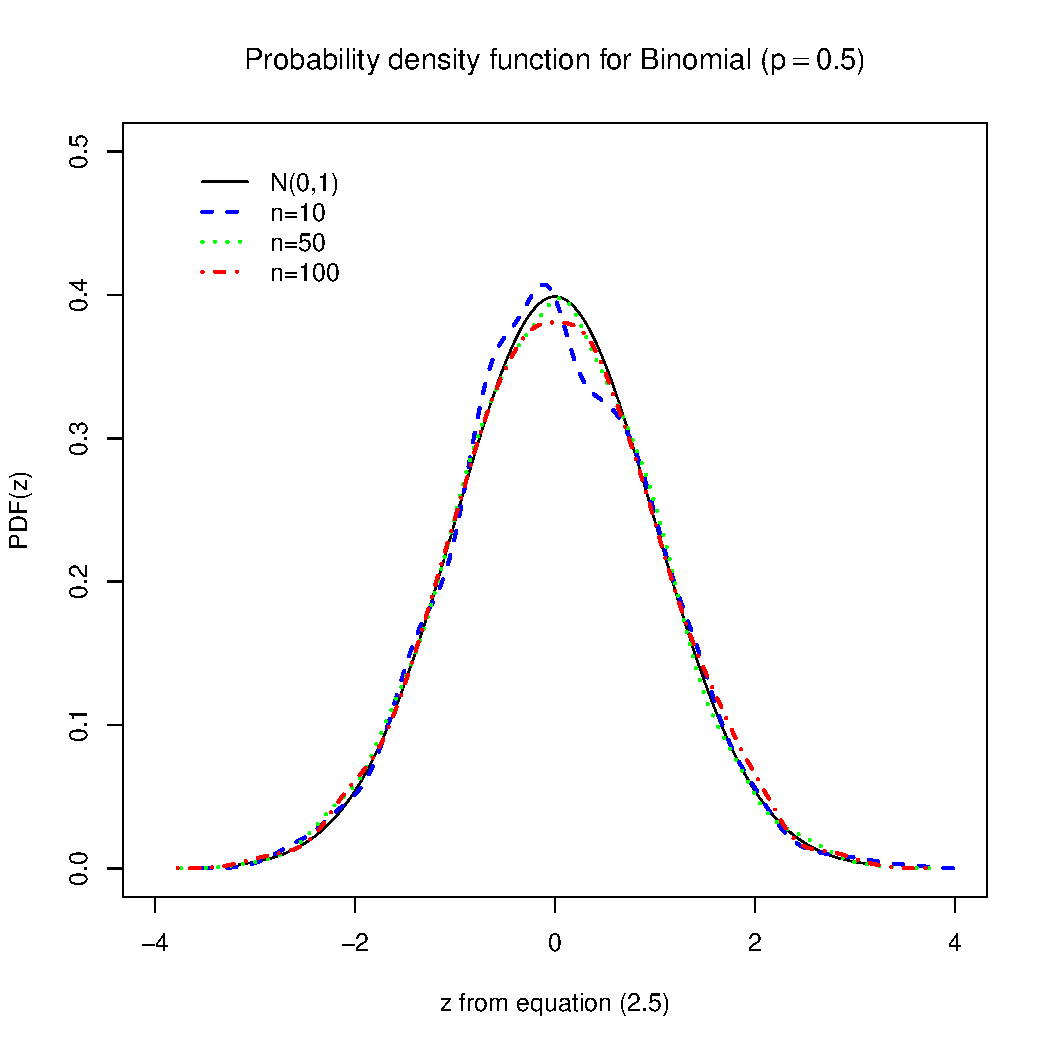
\includegraphics[width=0.49\textwidth]{Figures/binomial_PDF.pdf} \hfill
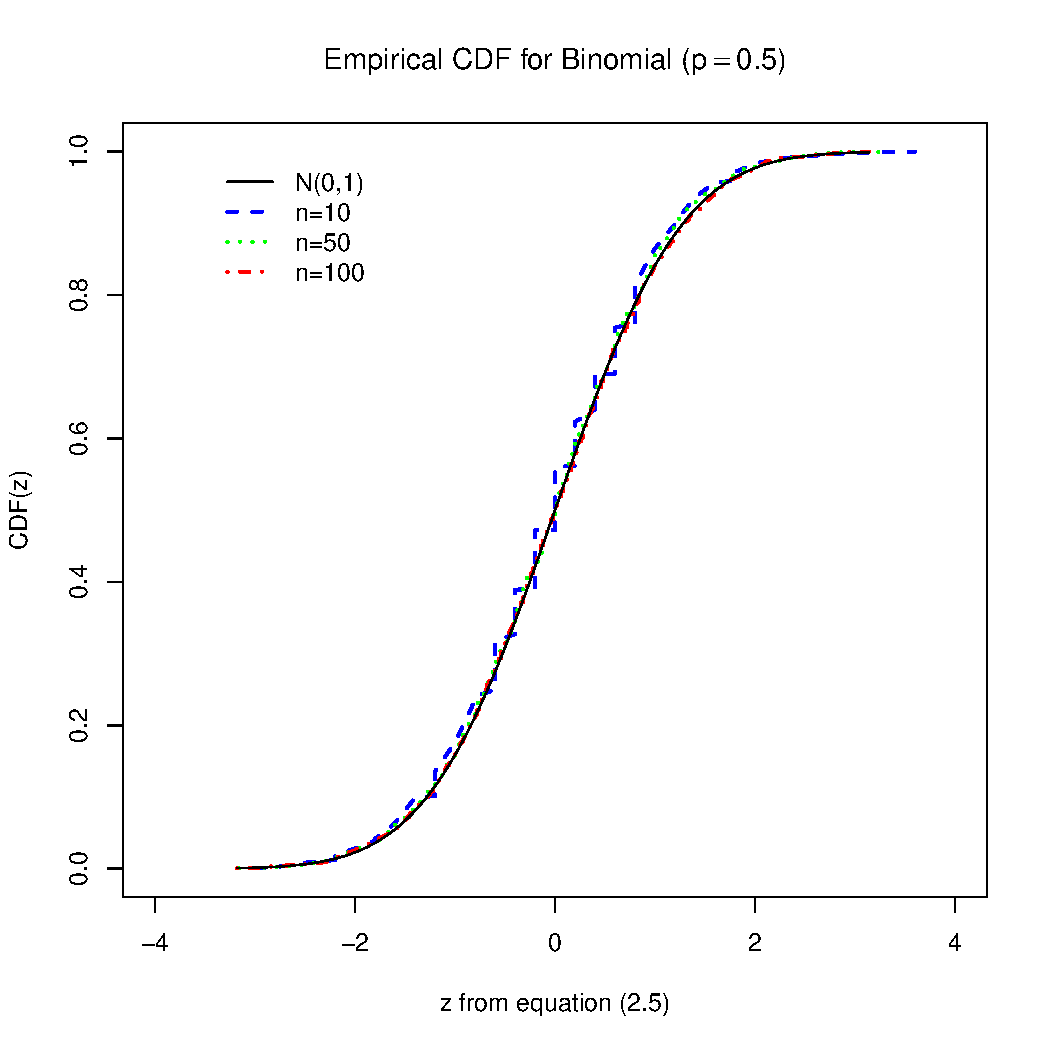
\includegraphics[width=0.49\textwidth]{Figures/binomial_CDF.pdf}\\
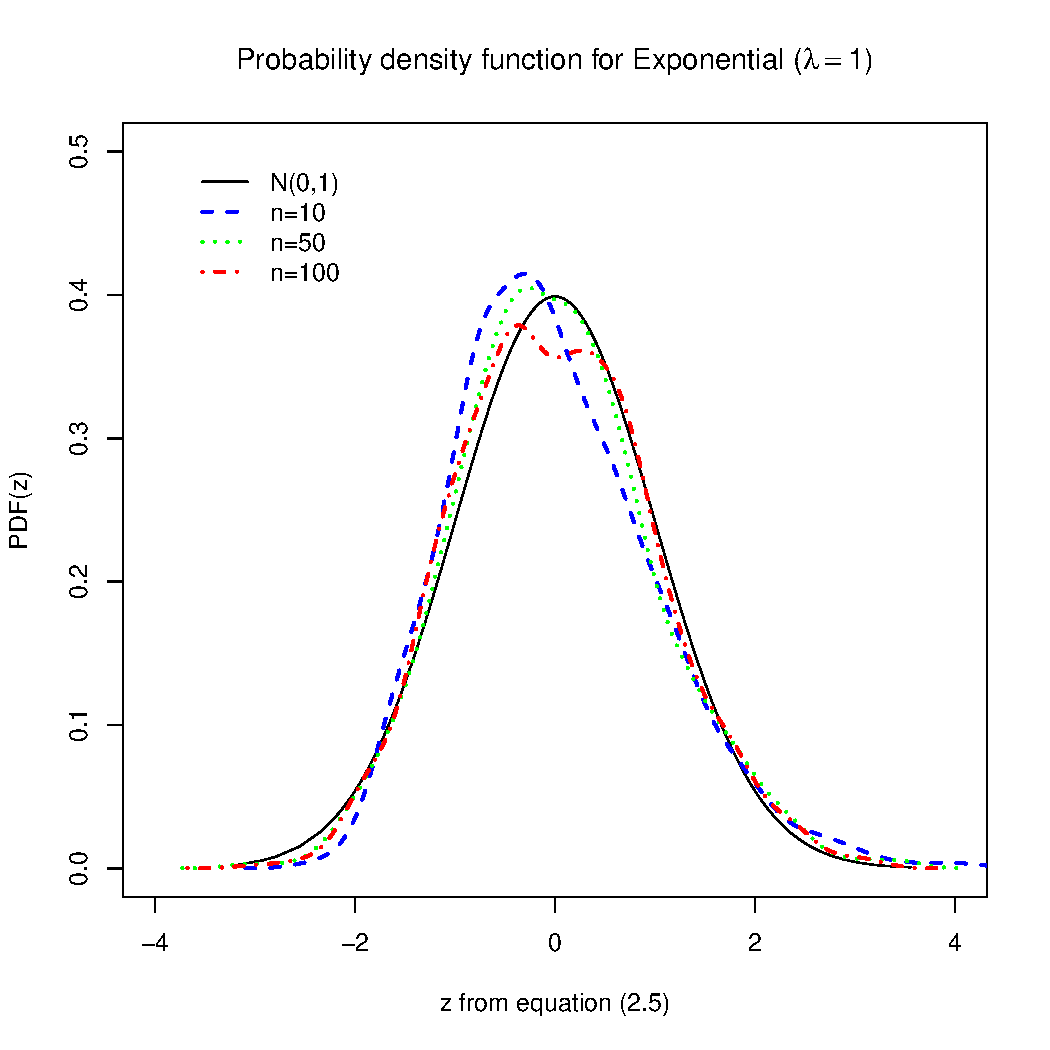
\includegraphics[width=0.49\textwidth]{Figures/expon_PDF.pdf} \hfill
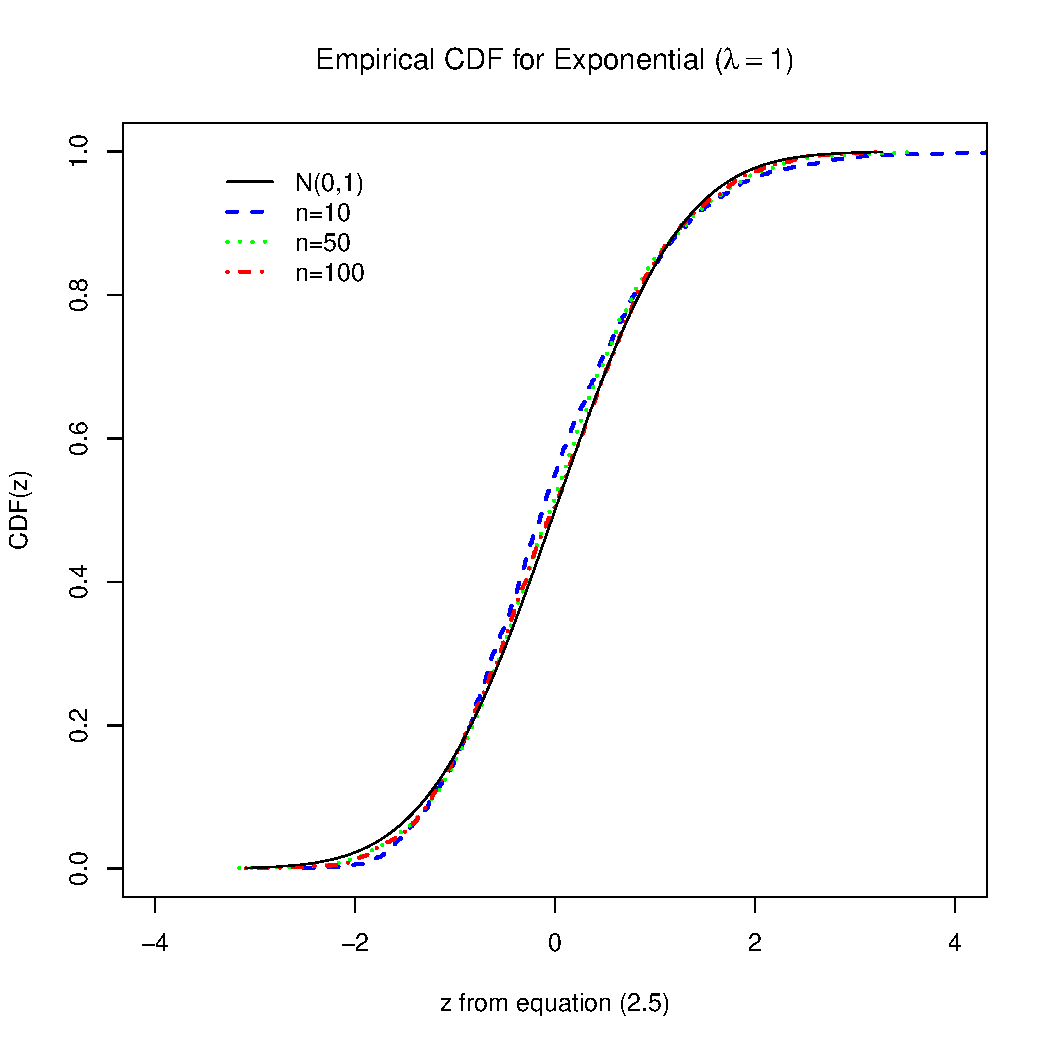
\includegraphics[width=0.49\textwidth]{Figures/expon_CDF.pdf}\\
\caption{Normal approximation for binomial and exponential distribution}\label{fig.CLT1}
\end{figure}

\begin{figure}[htp]
\centering
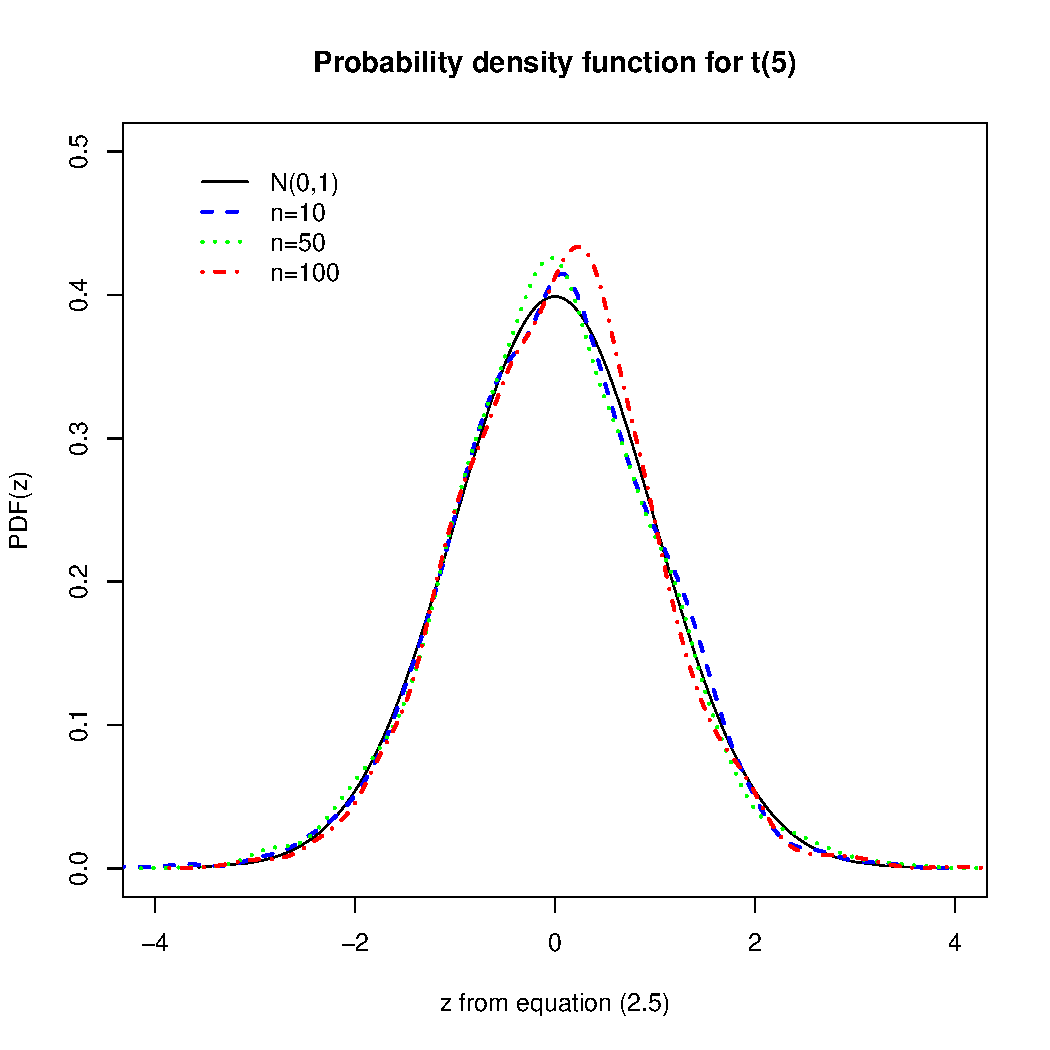
\includegraphics[width=0.49\textwidth]{Figures/t_PDF.pdf} \hfill
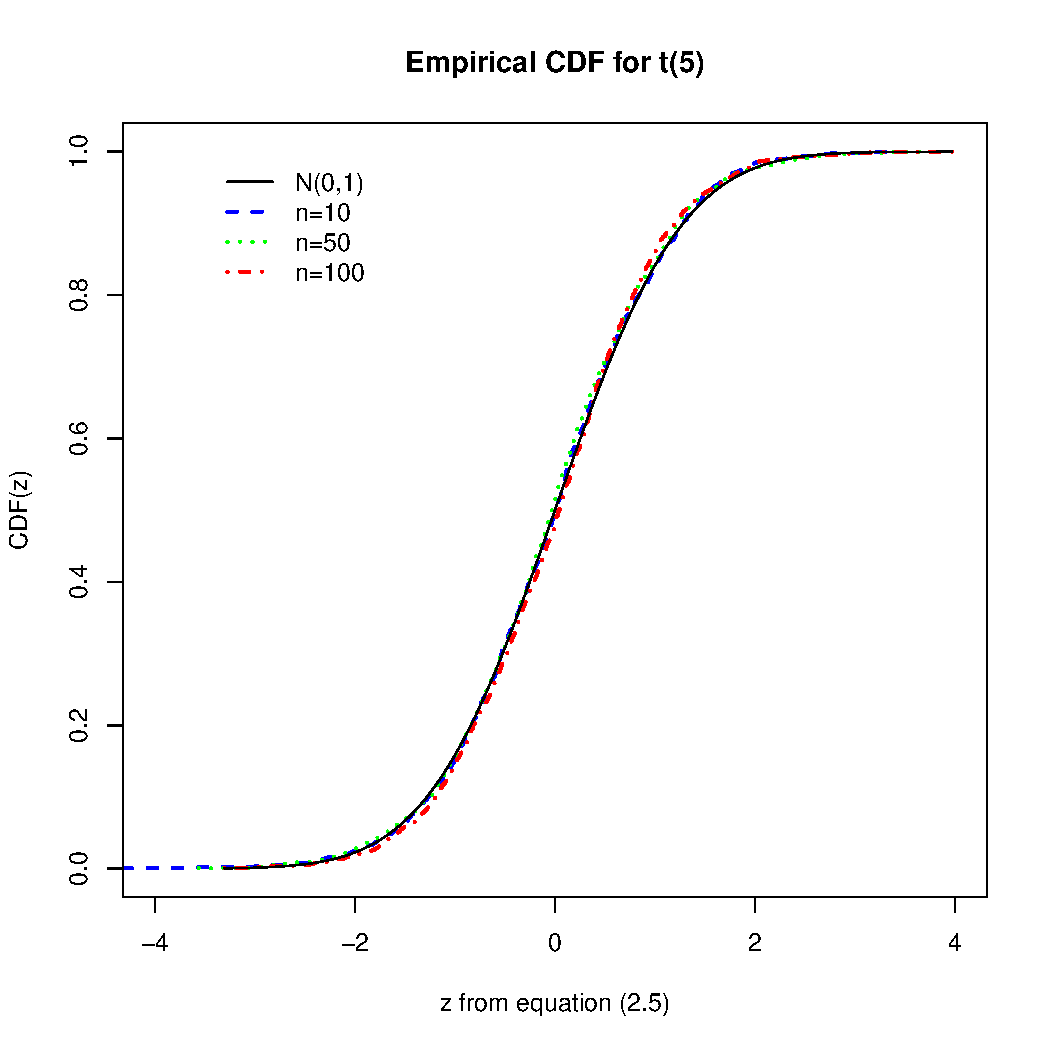
\includegraphics[width=0.49\textwidth]{Figures/t_CDF.pdf}\\
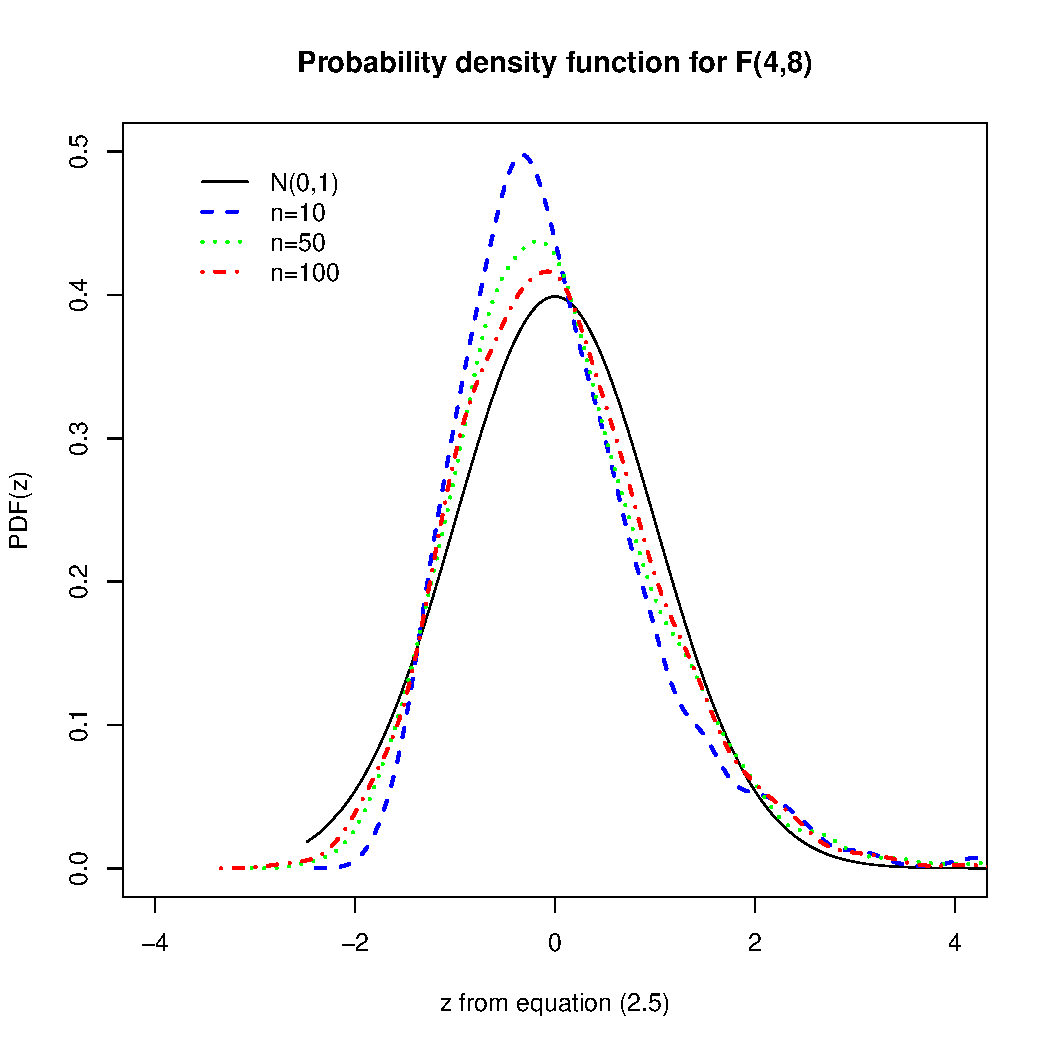
\includegraphics[width=0.49\textwidth]{Figures/f_PDF.pdf} \hfill
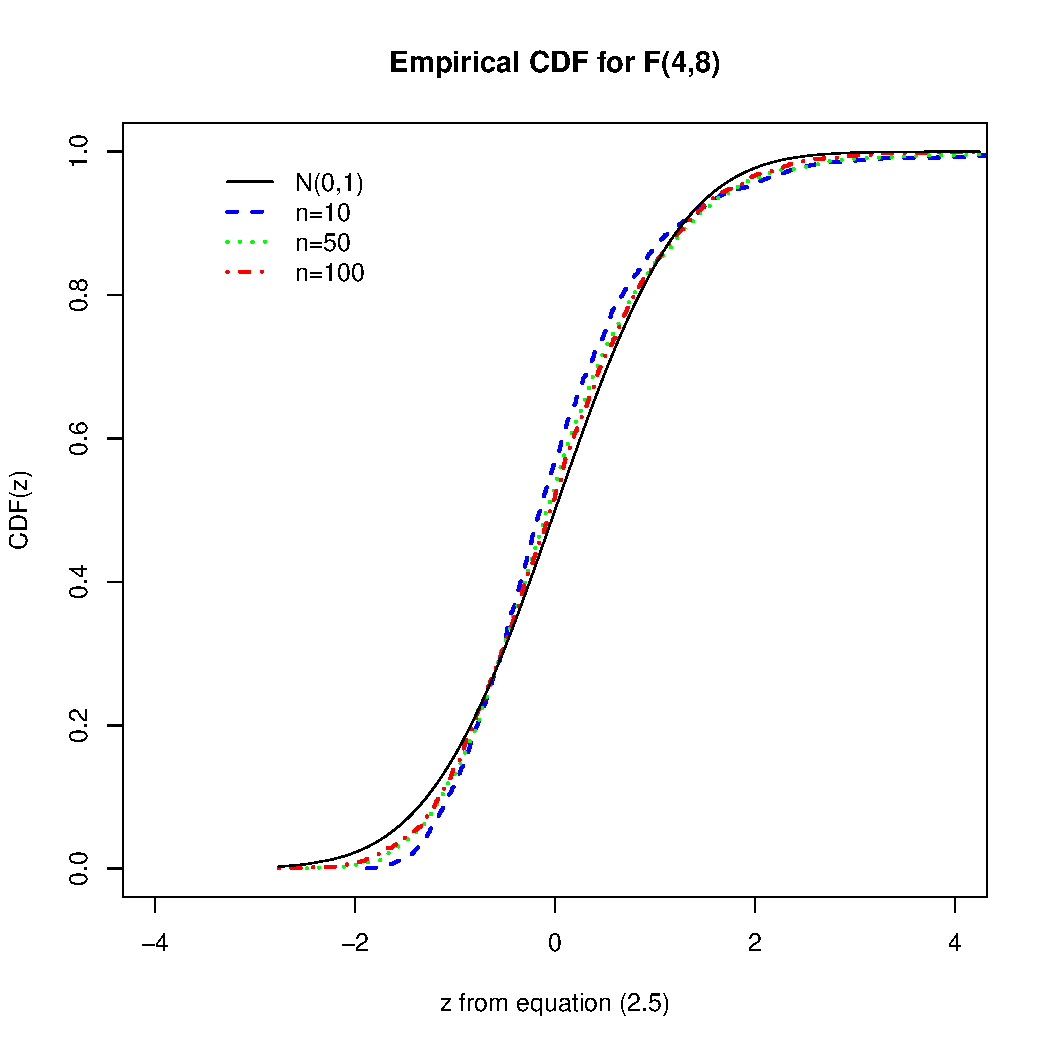
\includegraphics[width=0.49\textwidth]{Figures/f_CDF.pdf}\\
\caption{Normal approximation for $t$- and $F$-distribution}\label{fig.CLT2}
\end{figure}

\begin{figure}[htp]
\centering
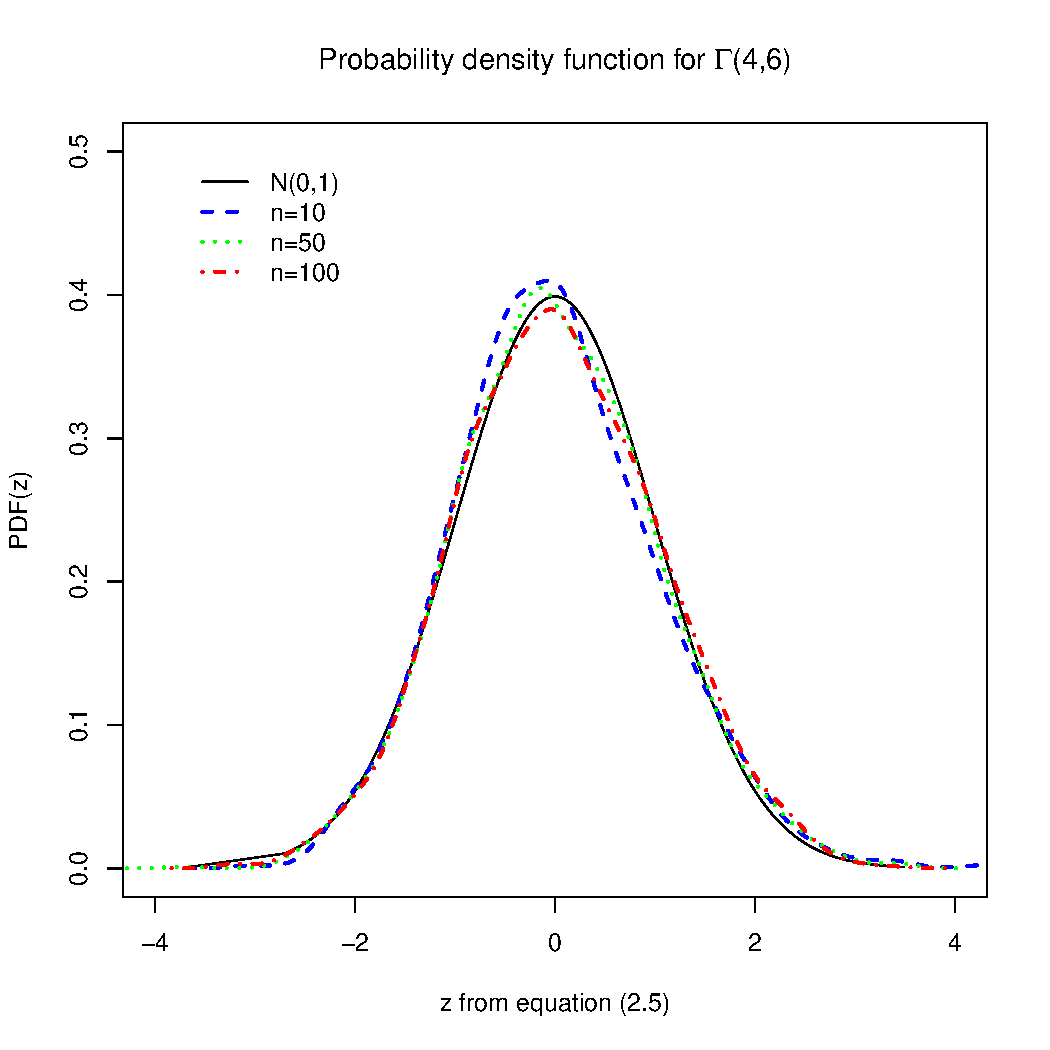
\includegraphics[width=0.49\textwidth]{Figures/gamma_PDF.pdf} \hfill
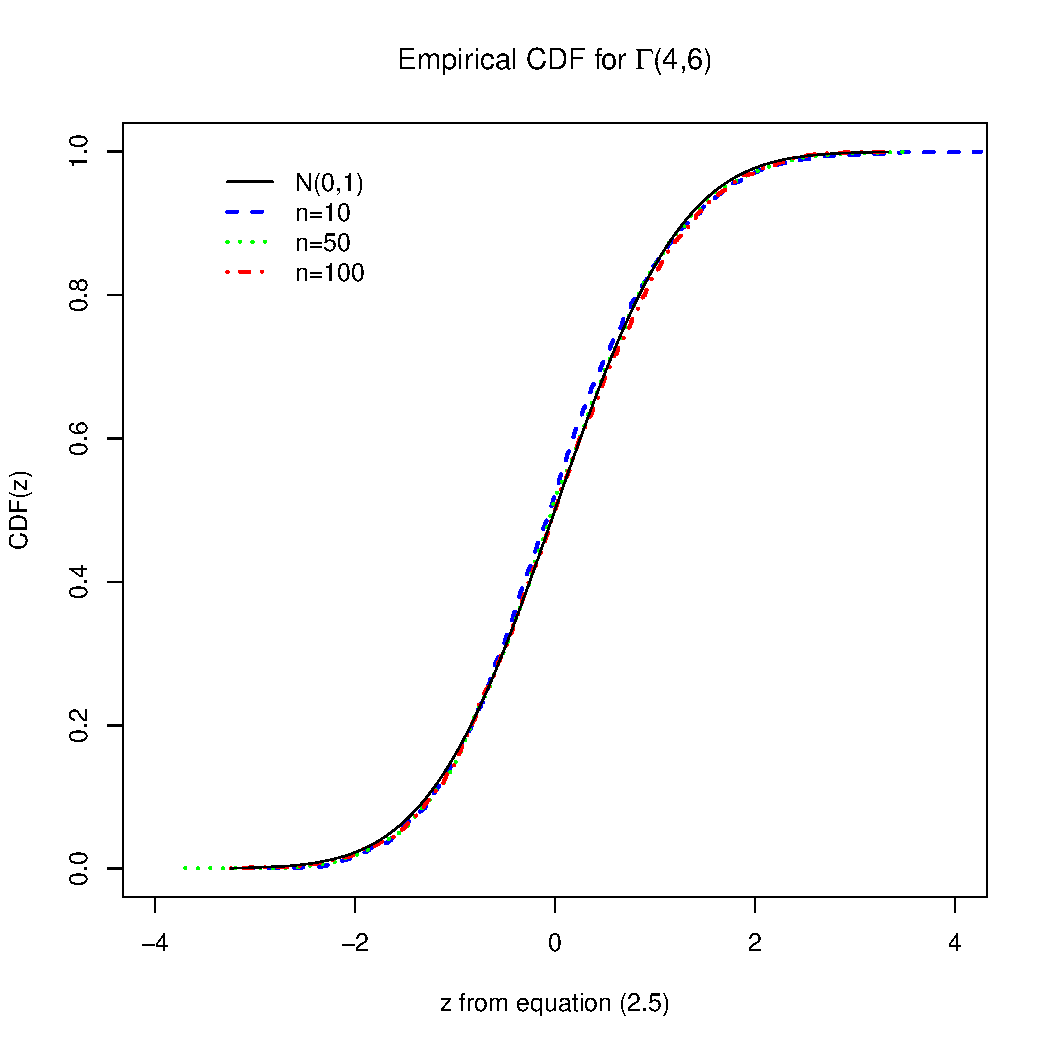
\includegraphics[width=0.49\textwidth]{Figures/gamma_CDF.pdf}\\
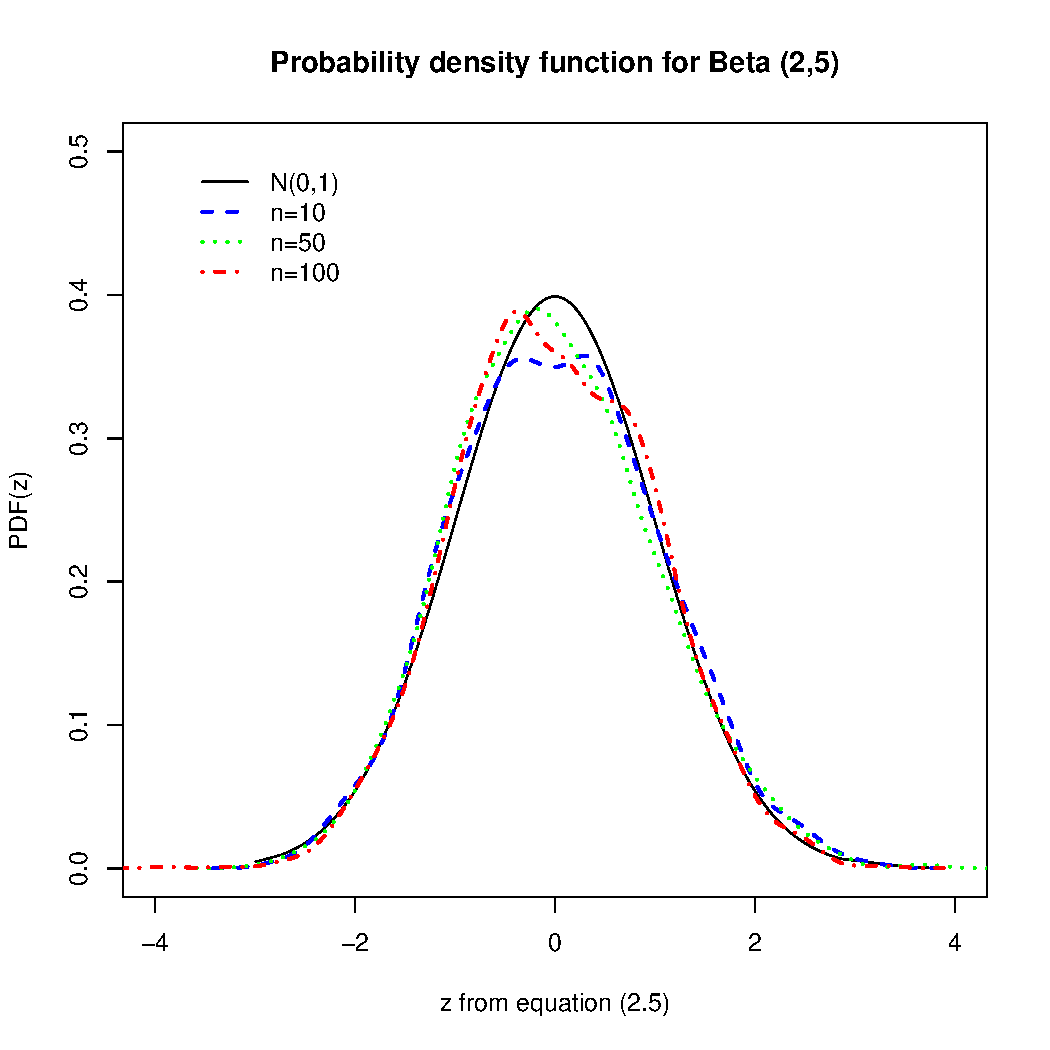
\includegraphics[width=0.49\textwidth]{Figures/beta_PDF.pdf} \hfill
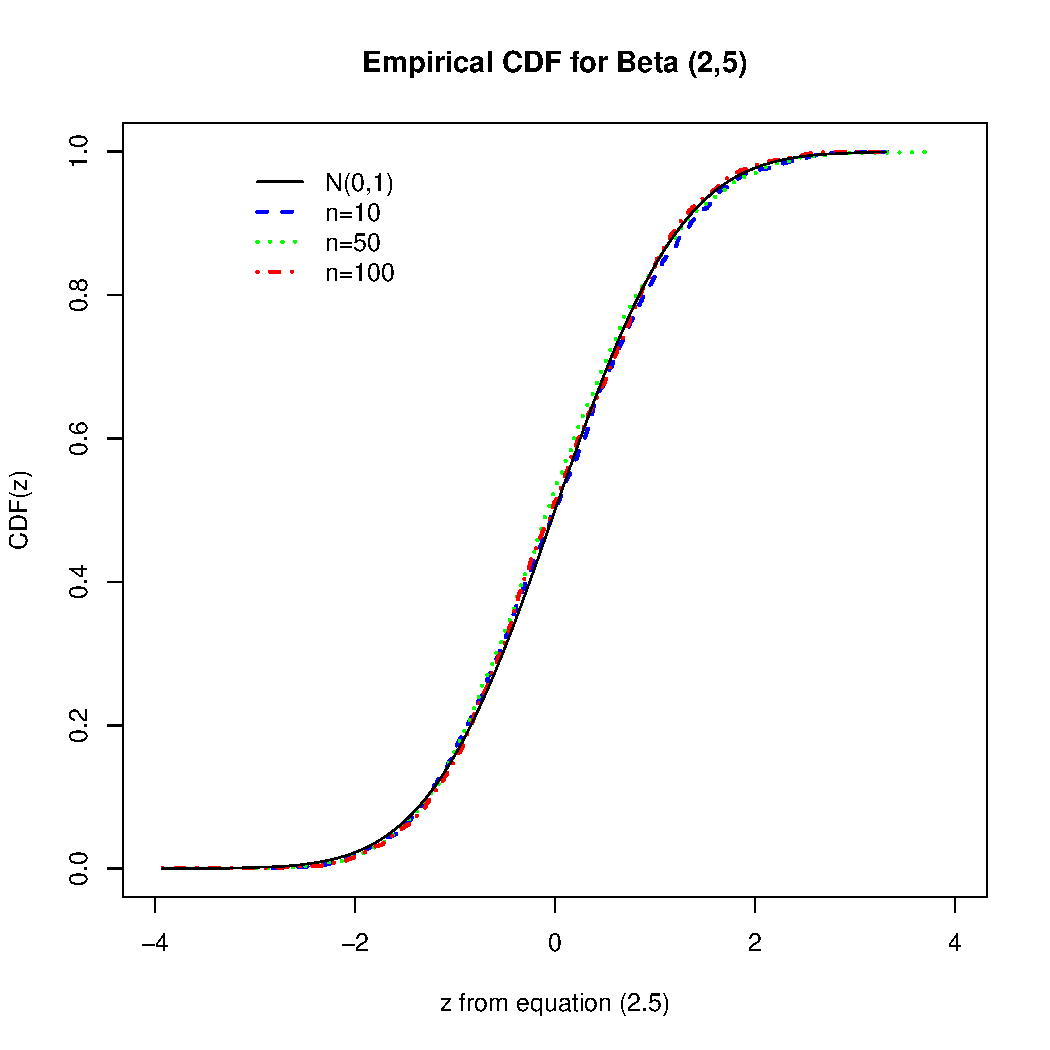
\includegraphics[width=0.49\textwidth]{Figures/beta_CDF.pdf}\\
\caption{Normal approximation for $\Gamma$- and Beta distribution}\label{fig.CLT3}
\end{figure}

Overall, this exercise demonstrates how powerful the CLT really is; for all six different distributions, $1/\sqrt(n)$ times the sum of $n$ centered random variables approximately follows a normal distribution even at $n$ as small as 10. Figures~\ref{fig.CLT1} to figure~\ref{fig.CLT3} show the empirical distribution functions for the six distributions.

\begin{itemize}
\item[\emph{Binomial}] The approximation to the standard normal distribution increases dramatically at $n=50$ as the step function is still visible at $n=10$.
\item[\emph{Exponential}] CLT takes effect visibly at $n=50$
\item[\emph{t}] Even at $n=10$, the centered random variables from the $t$-distribution approximate N(0,1) well. It is hardly surprising since the two distributions are very similar except that the t-distribution displays wider tails.
\item[\emph{F}] Centering for random variables from the $F$-distribution approximates the normal distribution only at comparatively large $n$, with the CLT fully taking effect at $n=100$
\item[\emph{Gamma}] Centered random variables from the $\Gamma$-distribution approximate N(0,1) reasonably well at the smallest $n$ with the CLT kicking more reliably at $n=50$.
\item[\emph{Beta}] Even at $n=10$, the centered random variables from the Beta-distribution approximate N(0,1) well. However for this distribution, the CLT-threshold seems to depend significantly on the random seed and fluctuated in different simulations between $n=10$ and $n=50$.
\end{itemize}

In addition to discovering that the CLT becomes effective at relatively small $n$ for a variety of distributions, this exercise demonstrates the impact of the variance on the centering process. The $\chi^{2}(m)$ distribution approaches the N($m,2m$) as $m$ becomes large and its variance is $2m$.

\begin{figure}[htp]
\centering
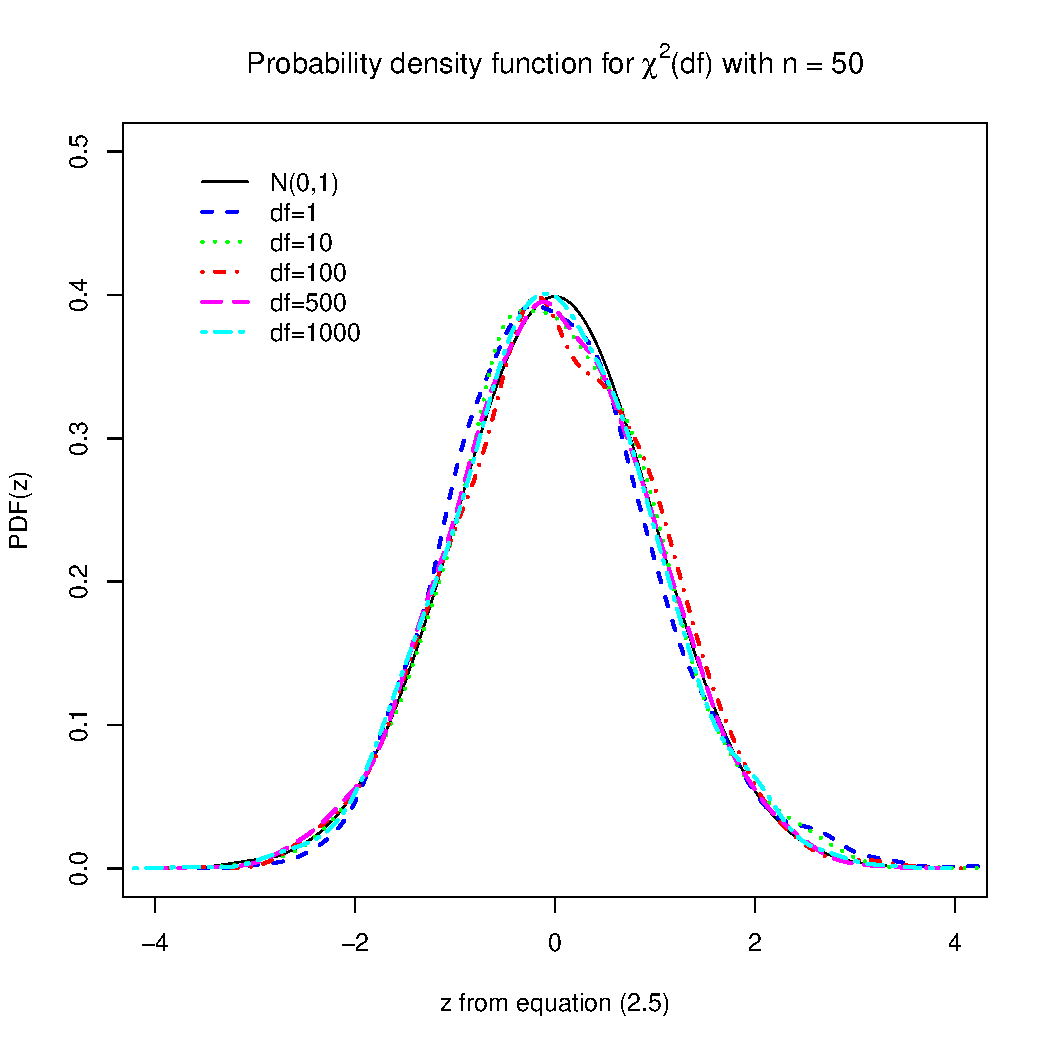
\includegraphics[width=0.75\textwidth]{Figures/chi1_PDF.pdf}
\caption{Normal approximation for $\chi^{2}$-distribution}\label{fig.CLT5}
\end{figure}

The different panels of figure~\ref{fig.CLT6} demonstrate that the \emph{variance} and \emph{sample size} work as \emph{substitutes} in the centering process; a higher variance requires a smaller sample size in order for the $\chi^{2}(m)$-distribution to approximate the standard normal distribution. This largely due to the fact that centering is achieved by subtracting the mean and dividing by the standard deviation. A large variance implies a large denominator which in turn implies that a smaller number of observations are required for the distribution to be asymptotically distributed as N(0,1).

\begin{figure}[htp]
\centering
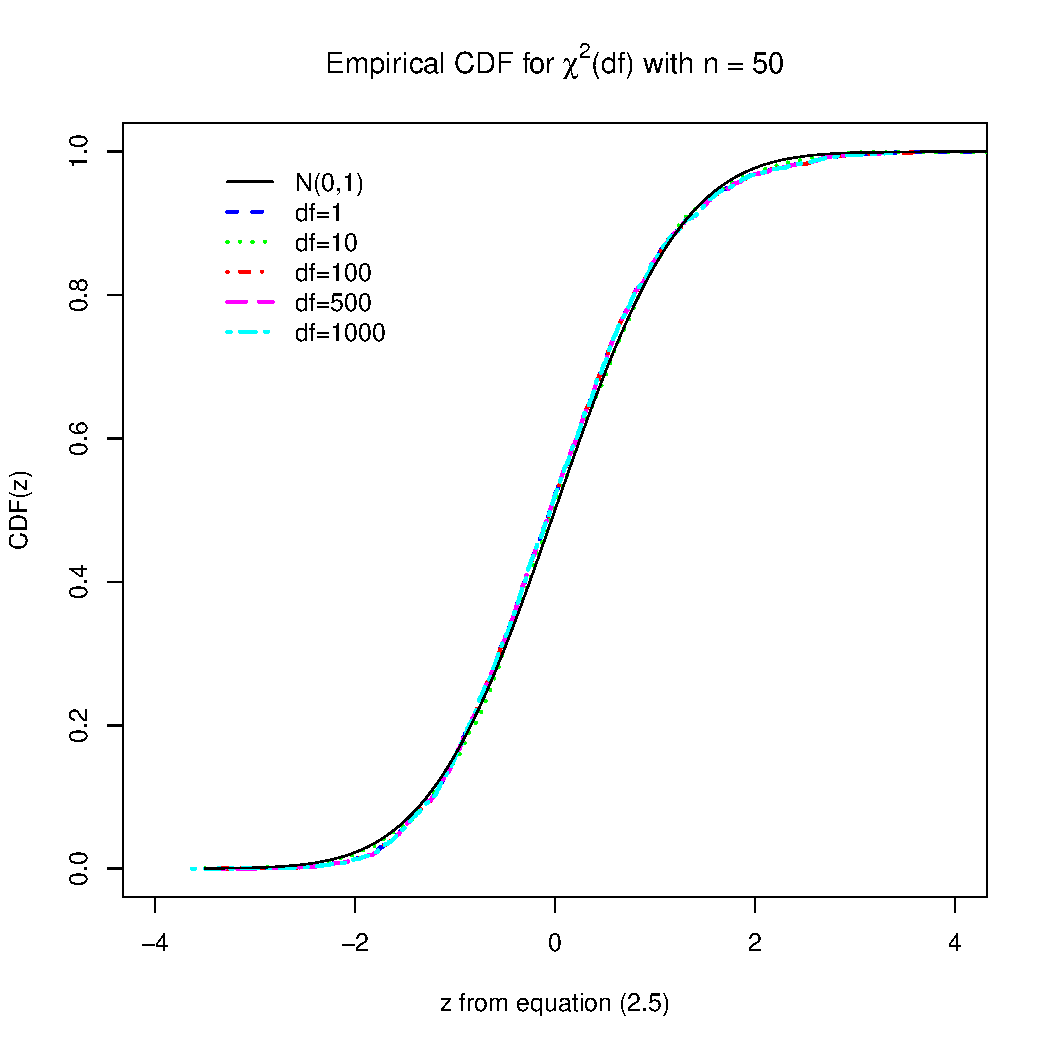
\includegraphics[width=0.49\textwidth]{Figures/chi2_CDF.pdf} \hfill
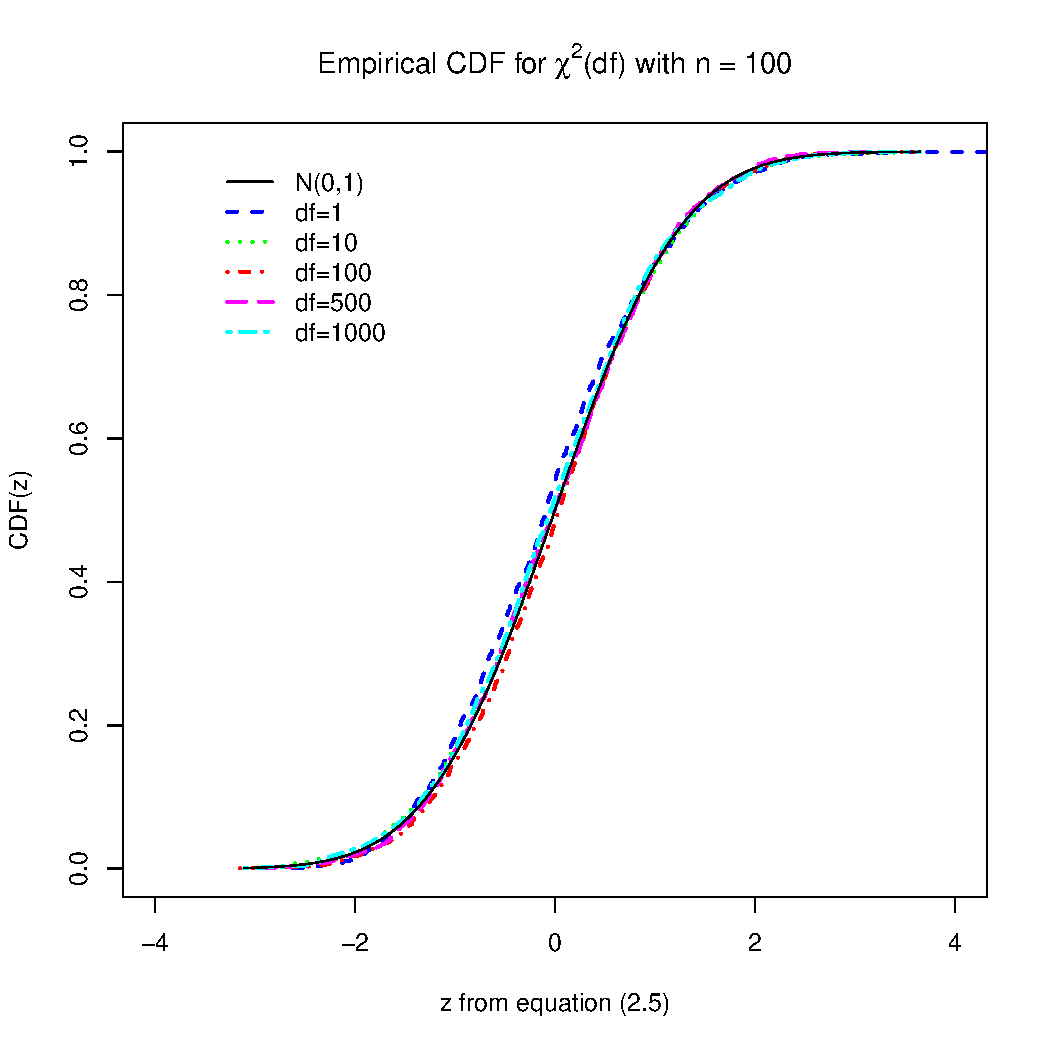
\includegraphics[width=0.49\textwidth]{Figures/chi3_CDF.pdf}\\
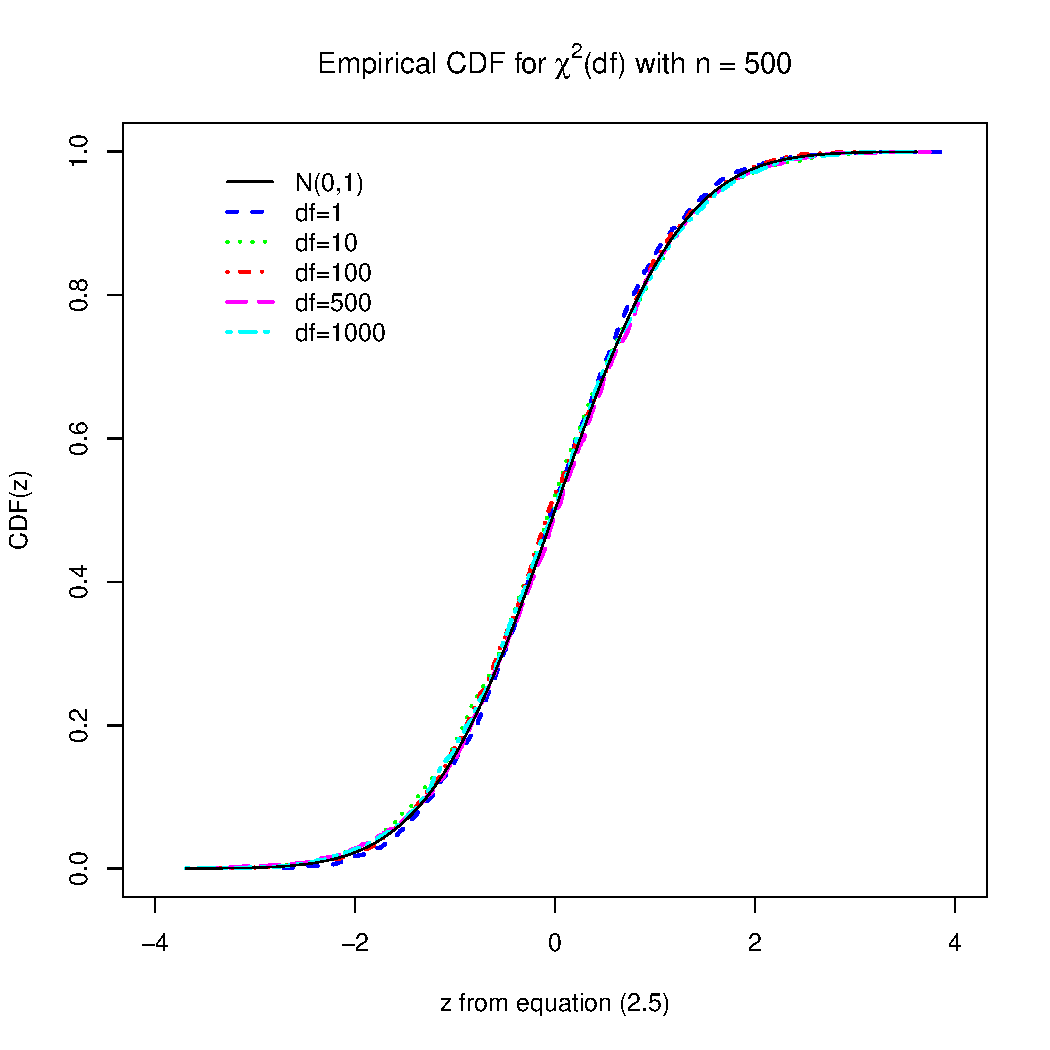
\includegraphics[width=0.49\textwidth]{Figures/chi4_CDF.pdf} \hfill
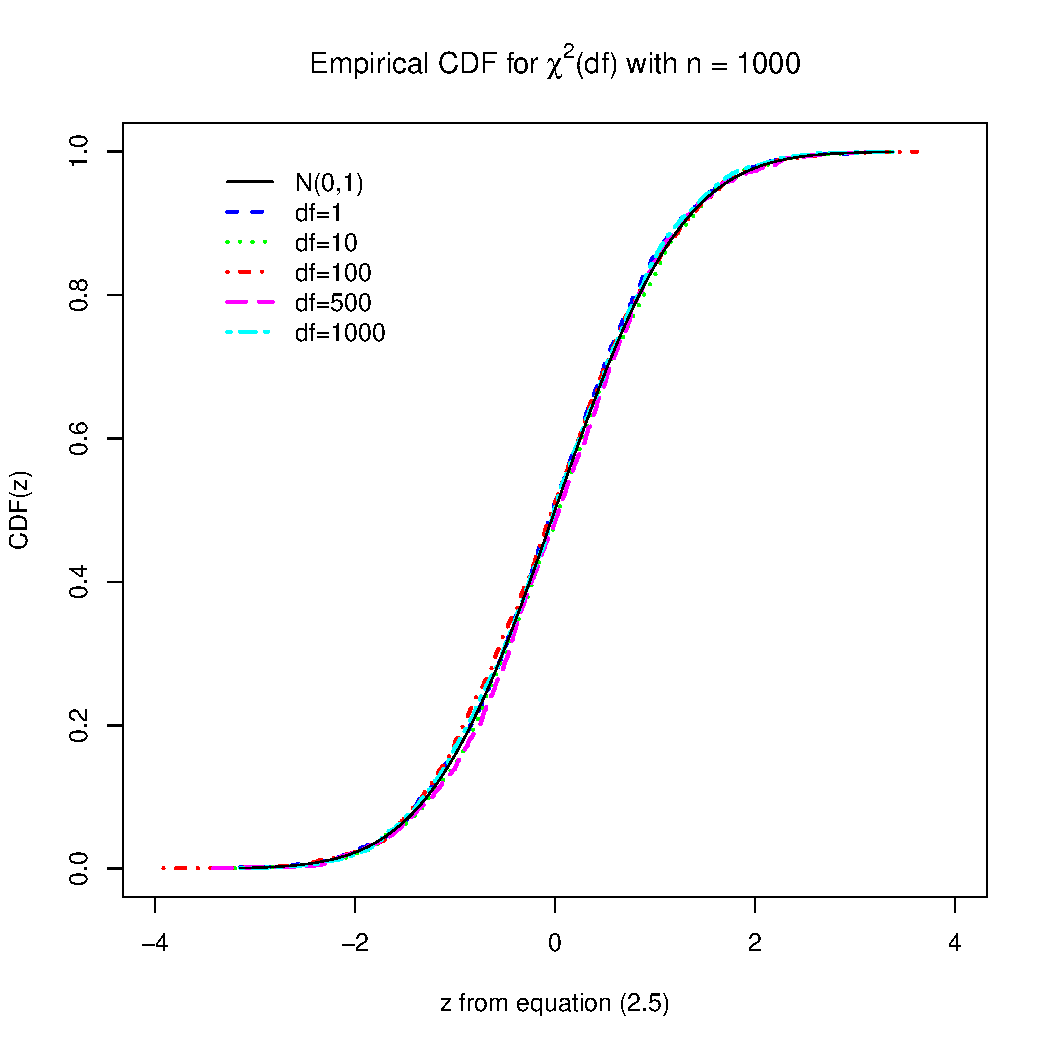
\includegraphics[width=0.49\textwidth]{Figures/chi5_CDF.pdf}\\
\caption{Variance impact and CLT for $\chi^{2}$-distribution}\label{fig.CLT6}
\end{figure}


\section{Matrix algebra}\label{chap_Review:Matrix}

\renewcommand\bibname{Further reading}
\begin{subappendices}
\bibliographystyle{econometrica}
\bibliography{Literature/OverLord}
\IfFileExists{Literature/Review.bbl}{\chapter{Review}\label{chap_Review}
\section{Preliminaries}\label{chap_Review:Prelim}
``Probability approach in econometrics'' by Trygve \citet{Haavelmo1944} stands at the beginning of a paradigm shift in statistical thinking; the \emph{classical} interpretation of statistics is giving way to the \emph{frequentist} interpretation. Under the classical interpretation, probabilities are linked to the principle of indifference and statistical events are governed by natural symmetry (e.g. coin tosses, die etc.) This constraining set-up of what gives rise to probabilities is one of the key problems of the classical view. 

Under the frequentist interpretation on the other hand, probabilities of events are linked to the frequency with which a given event is observed. This implies that

$$P(x)= \lim\limits_{n_{t} \rightarrow \infty} \frac{n_{x}}{n_{t}},$$ 

where $n_{x}$ is the number of observed trials and $n_{t}$ is the total number of trials. This probabilistic approach to statistics, which includes Bayesian statistics\index{Bayesian statistics}, represents the world in terms of ``degrees of belief'' (Bayesian priors).

More formally, Bayes' Theorem is expressed as the conditional probability of occurence A given B such that $$P(A|B) = \frac{P(B|A)P(A)}{P(B)}.$$\index{Bayes' Theorem|see{Bayesian statistics}}


\section{Statistics and probability theory}\label{chap_Review:Stats}
\subsection{Types of random variables}
A random variable, usually written as $X$, is a variable whose possible values are numerical outcomes of a random phenomenon. A random variable $X$  is a (real) number with the following characteristics:

\begin{inparaenum}[\itshape a\upshape)]
\item the value of $X$ is unknown;
\item the possible values $X$ can take are known; the set of such values is called support and denoted by $\bm{\mathcal{S}}_{X}$;
\item if $\bm{\mathcal{A}}$  is a subset of the set of real numbers $\mathbb{R}$  (i.e. $\bm{\mathcal{A}}\subseteq \mathbb{R}$), we know the probability that $X$ belongs to $\bm{\mathcal{A}}$ which is denoted by $P(X\in\bm{\mathcal{A}})$.
\item If (and when) the value $x$ of $X$  becomes known, such that $x=X$, $x$ is then referred to as the realization of $X$. Hence, the support $\bm{\mathcal{S}}_{X}$  is the set of all possible realizations of $X$.
\end{inparaenum}

Random variables generally fall into two categories, discrete and continuous:

\begin{itemize}
\item Discrete random variables\index{random variable!discrete}: Takes on only a countable number of distinct values such as $0,1,2,3,4 \ldots$ Discrete random variables are usually (but not necessarily) counts. If a random variable can take only a finite number of distinct values, then it must be discrete.
\item Continuous random variables\index{random variable!continuous}: Takes an infinite number of possible values. Continuous random variables are usually measurements. Examples include height, weight, the amount of sugar in an orange, the time required to run a mile.
\end{itemize}

In addition to distinguishing between discrete and continuous random variables, we can also categorise random variables into \emph{qualitative} variables or \emph{quantitative} variables. Qualitative\index{qualitative variable|see{random variable}} or categorical variables are either nominal, ordinal or dichotomous. 

\begin{itemize}
\item Nominal variables: \index{random variable!nominal}\index{categorical variable|see{random variable}} A variable for mutually exclusive, but not ordered categories such as, for example, your study might compare five different types of suburbs (inner-ring suburbs, commuter suburb, sitcom suburb, high-income suburb, minority suburb). 
\item An ordinal variable\index{random variable!ordinal} is a random variable where the order matters but not the difference between values. For example, quality of life rankings might express how nice a place is on a scale of 1 to 10. A score of 7 means a nicer place that a score of 5, and that is more than a score of 3. But the difference between the 7 and the 5 may not be the same as that between 5 and 3. The values simply express an order. 
\end{itemize}

Quantitative variables\index{quantitative variable|see{random variable}} are either interval variables where differentiation or transformation preserves the units (such as in the case of temperature measurements in C, F) or ratio variables where a value of 0 means that nothing of that variable is present. Thus temperature measured in Kelvin or height, for example, are ratio variables.

\begin{itemize}
\item An interval variable\index{random variable!interval} is a measurement where the difference between two values is meaningful. The difference between a temperature of 100 degrees and 90 degrees is the same difference as between 90 degrees and 80 degrees. 
\item When working with ratio variables\index{random variable!ratio}, you can look at the ratio of two measurements. A weight of 4 grams is twice a weight of 2 grams, because weight is a ratio variable. A temperature of 100 degrees Celsius is not twice as hot as 50 degrees C, because temperature C is not a ratio variable. Similarly, a pH of 3 is not twice as acidic as a pH of 6, because pH is an interval variable and not a ratio variable. 
\end{itemize}

\begin{table}[htp] 
\centering
\caption{Basic statistical operations by variable type}
\footnotesize
\begin{tabular}{lcccc}\label{tbl_Vars}
\\ \hline
\hline
&\multicolumn{4}{c}{\emph{Random variable type}}\\
\emph{Operation}&Nominal&Ordinal&Ratio&Interval\\
\cline{2-5}
Frequency distribution&Yes&Yes&Yes&Yes\\
Median and percentiles&No&Yes&Yes&Yes\\
Addition/subtraction&No&No&Yes&Yes\\
Mean, standard deviation, standard error of the mean&No&No&Yes&Yes\\
Ratio/coefficient of variation&No&No&No&Yes\\
\hline
\hline \\
\normalsize
\end{tabular}
\end{table}


\subsection{Expectations}
\subsubsection{Expectation of a discrete random variable}
\begin{eqnarray}
\mathbb{E}(X) &=& x_{1}p_{1} + x_{2}p_{2} + x_{3}p_{3} +\ldots + x_{n}p_{n}\nonumber \\
&=& \sum^{n}_{i=1}x_{i}p_{i}
\end{eqnarray}

Recall that in a finite sample, $\mathbb{E}(X)$ denotes the sample mean and the sum of all probabilities must be equal to one, i.e. $\sum_{i}p_{i}=1$.

\paragraph{Example} Consider the following gamble where an unbiased coin with heads ($H$) and tails ($T$) is tossed $n$ times until tails ($T$) appears. If $T$ shows up at the $n$-th toss, the payoff is $\$2^{n-1}$. How much would you be willing to put up as a wager to participate in this game?

\begin{eqnarray*}
\mathbb{E}(X) &=& \$2^{0}\cdot\frac{1}{2} + \$2^{1}\cdot\frac{1}{2}\cdot\frac{1}{2} + \$2^{2}\cdot\frac{1}{2}\cdot\frac{1}{2}\cdot\frac{1}{2} + \ldots \\
&=& \$1\cdot\frac{1}{2} + \$2\cdot\frac{1}{4} + \$4\cdot\frac{1}{8} + \ldots\\
&=& \sum^{\infty}_{i=1}\$ 0.5 = \$\infty
\end{eqnarray*}

This is the \emph{St. Petersburg paradox}\index{St. Petersburg paradox} famously defined and described by Daniel Bernoulli\index{Bernoulli, Daniel} (Swiss mathematician (1700--1782), father of modern fluid dynamics) to illustrate the failure of expected value principle (as opposed to expected utility) in decision theory under uncertainty. Thus the expected payout value of a St. Petersburg game is an infinite amount, yet clearly the willingness to pay (WTP)\index{WTP|see{willingness to pay}}\index{willingness to pay} to participate in such a game must be (much) less than its expected value. The classical resolution of the paradox thus involves the explicit introduction of a utility function\index{utility}, an expected utility hypothesis, and the presumption of diminishing marginal utility of money. This implies $\mathbb{E}(U) < \mathbb{E}(X)$.

\paragraph{Example} What is the expected value of throwing a single die (or a pair of dice)?

\begin{eqnarray*}
\mathbb{E}(X) = \frac{1}{6}\cdot 1 + \frac{1}{6}\cdot 2 + \frac{1}{6}\cdot 3 + \ldots + \frac{1}{6}\cdot 6 = 3.5
\end{eqnarray*}

Thus the sample mean $\mu_{X} = 3.5$ and analogously, for a pair of dice, $\mu_{X} = 7$. A table with the bivariate probabilities is shown in table~\ref{tbl_Dice} below:


\begin{table}[htp] 
\centering
\caption{Bivariate probabilities for a pair of dice and expected value of $X$}
\footnotesize
\bigskip
\begin{tabular}{lll|lll}\label{tbl_Dice}
\\ \hline
\hline
$X$&$p$&$Xp$&$X$&$p$&$Xp$\\
\hline
$x_{1}$ & $p_{1}$ & $x_{1}p_{1}$ & 2 & 1/36 & 2/36\\
$x_{2}$ & $p_{2}$ & $x_{2}p_{2}$ & 3 & 2/36 & 6/36\\
$x_{3}$ & $p_{3}$ & $x_{3}p_{3}$ & 4 & 3/36 & 12/36\\
$\ldots$ & $\ldots$ & $\ldots$ & 5 & 4/36 & 20/36\\
$\ldots$ & $\ldots$ & $\ldots$ & 6 & 5/36 & 30/36\\
$\ldots$ & $\ldots$ & $\ldots$ & 7 & 6/36 & 42/36\\
$\ldots$ & $\ldots$ & $\ldots$ & 8 & 5/36 & 40/36\\
$\ldots$ & $\ldots$ & $\ldots$ & 9 & 4/36 & 36/36\\
$\ldots$ & $\ldots$ & $\ldots$ & 10 & 3/36 & 30/36\\
$\ldots$ & $\ldots$ & $\ldots$ & 11 & 2/36 & 22/36\\
$x_{n}$ & $p_{n}$ & $x_{n}p_{n}$ & 12 & 1/36 & 6/36\\

\hline
\multicolumn{3}{l}{Total: $\mathbb{E}(X)=\sum^{n}_{i=1}x_{i}p_{i}$}&&\multicolumn{2}{r}{252/36 = 7}\\
\hline \\
\normalsize
\end{tabular}
\end{table}


\subsection{Expectations rules}
\begin{enumerate}
\item $\mathbb{E}[X + Y + Z] = \mathbb{E}(X) + \mathbb{E}(Y) + \mathbb{E}(Z);$
\item $\mathbb{E}[bX] = b\mathbb{E}(X);$
\item $\mathbb{E}[b] = b$
\end{enumerate}

\paragraph{Example} Different rules can be combined, e.g. $\mathbb{E}[a + bX] = a + b\mathbb{E}(X)$. Let a normally distributed random variable $V$ can have any mean $\mu$ and any positive variance $\sigma^{2}$. Such a random variable is said to follow the $\mathcal{N}(\mu, \sigma^{2})$ distribution. A standard normal variable therefore has the $\mathcal{N}(0, 1)$ distribution.

Suppose that $V$ has the standard normal distribution. What are the corresponding mean $\mu$ and variance $\sigma^{2}$ of a new random variable $Z \equiv \mu + \sigma V$? For the mean, we use the fact that $\mathbb{E}\left[V\right]=0$ which yields

\begin{eqnarray*}
\mathbb{E}\left[Z\right] &=& \mathbb{E}\left[\mu + \sigma V\right] = \mathbb{E}\left[\mu\right] + \mathbb{E}\left[\sigma V\right] = \mu + \sigma\mathbb{E}\left[V\right]\\
&=& \mu.
\end{eqnarray*}

Similarly, when deriving the variance, recall that $\text{var}(V)=\mathbb{E}\left[V^{2}\right]=1$ such that

\begin{eqnarray*}
    \mathbb{E}\left[(Z-E\left[Z\right])^{2}\right] &=& \mathbb{E}\left[Z^{2}-2Z\mathbb{E}\left[Z\right]+ (\mathbb{E}\left[Z\right])^{2}\right]= \mathbb{E}\left[Z^{2} -2Z\mu + \mu^{2}\right]\\
    &=& \mathbb{E}\left[Z^{2}\right] -2\mu\mathbb{E}\left[Z\right] + \mathbb{E}\left[\mu^{2}\right]= \mathbb{E}\left[Z^{2}\right] -2\mu^{2} + \mu^{2}\\
    &=& \mathbb{E}\left[(\mu^{2}+ 2\mu\sigma V + \sigma^{2}V^{2})\right] -\mu^{2} \\
    &=& \mu^{2} + 2\mu\sigma \mathbb{E}\left[V\right] +\sigma^{2}\mathbb{E}\left[V^{2}\right] -\mu^{2} =  \\
    &=& \sigma^{2}.
    \end{eqnarray*}


\subsubsection{Variance of a discrete random variable}
\begin{eqnarray}
\textrm{Var}(X) = \sigma^{2}_{X} &=& \mathbb{E}[(X-\mu_{X})^{2}]\nonumber \\
&=& (x_{1} - \mu_{X})^{2}p_{1} + (x_{2} - \mu_{X})^{2}p_{2} + \ldots + (x_{n} - \mu_{X})^{2}p_{n} \nonumber\\
&=& \sum^{n}_{i=1}(x_{i} - \mu_{X})^{2}p_{i}
\end{eqnarray}

Derivation of alternative expression for the variance:

\begin{eqnarray}
\textrm{Var}(X) = \sigma^{2}_{X} &=& \mathbb{E}[(X-\mu_{X})^{2}]\nonumber \\
&=& \mathbb{E}[(X-\mu_{X})((X-\mu_{X})] \nonumber\\
&=& \mathbb{E}[X^{2}-2\mu_{X}X + \mu_{X}^{2}] \nonumber\\
&=& \mathbb{E}[X^{2}] -\mathbb{E}[2\mu_{X}X] + \mathbb{E}[\mu_{X}^{2}] \nonumber\\
&=& \mathbb{E}[X^{2}] -2\mu_{X}\mathbb{E}[X] + \mu_{X}^{2} \nonumber\\
&=& \mathbb{E}[X^{2}] -2\mu_{X}^{2} + \mu_{X}^{2} = \mathbb{E}[X^{2}] - \mu_{X}^{2}
\end{eqnarray}

\subsubsection{Fixed and random components of variables}
Let the random variable $X$ be decomposed into two parts, namely a constant mean $\mu_{X}$ and a variable component $u$. Think of $u$ as measurement error or a stochastic disturbance term with $\mathbb{E}(u)= \mathbb{E}(X-\mu_{X}) = \mathbb{E}(X) -\mu_{X}= 0$.

Because all variation in $X$ is due to $u$, the variance of $X$, $\sigma^{2}_{X}$, is identical to the variance of the disturbance term, $\sigma_{u}$. More formally, we can write

\begin{eqnarray*}
\sigma^{2}_{X}&=& \mathbb{E}[(X-\mu_{X})^{2}] = \mathbb{E}(u^{2})\\
\sigma^{2}_{u}&=& \mathbb{E}[(u-\mu_{u})^{2}] = \mathbb{E}(u^{2}).
\end{eqnarray*}

\section{Probability distributions}
All random variables (discrete and continuous) have a probability density function (PDF)\index{PDF|see{density function}}\index{density function!probability} and a cumulative density function (CDF)\index{CDF|see{density function}}\index{density function!cumulative}. These are functions that give the probability that the random variable $X$ is less than or equal to $x$, for every value $x$. For a discrete random variable, the cumulative distribution function is found by summing up the probabilities.


\begin{figure}[htp]
\caption{Probability density function with $f(x)\equiv F'(x)$ }\label{fig_PDF}
\begin{center}
\includegraphics[width=0.7\textwidth]{"Figures/PDFjc"}
\end{center}
\footnotesize
\end{figure}


\begin{figure}[htp]
\caption{Cumulative density function with $\int f(x) \equiv F(x)$}\label{fig_CDF}
\begin{center}
\includegraphics[width=0.7\textwidth]{"Figures/CDFjc"}
\end{center}
\footnotesize
\end{figure}

Using R, it is fairly straightforward to produce the PDF and CDF of a standard normal distribution:

\begin{lstlisting}
#Probability density function with shaded area
cord.x <- c(-2,seq(-2,-1,0.01),-1) 
cord.y <- c(0,dnorm(seq(-2,-1,0.01)),0) 
curve(dnorm(x,0,1),xlim=c(-3,3),main='PDF', xlab='Marginal Density') 
polygon(cord.x,cord.y,col='blue')


#Cumulative density function
x <- rnorm(10000)
plot(ecdf(x), ylab="Probability")
\end{lstlisting}


\begin{eqnarray*}
\text{Pr.}[A\leq x\leq B]=\int_{A}^{B} f(x)dx
\end{eqnarray*}

$\therefore$ we can write the expectation of a continuous random variable as:

\begin{eqnarray*}
\text{CDF}=\int_{-\infty}^{x} f(x)dx = F(B)-F(A)=\int_{-\infty}^{x}F'(x)dx
\end{eqnarray*}

Equivalently, in the case of a continuous random variable the variance can be expressed as:

\begin{eqnarray}
\mathbb{E}\left[x\right]=\int x f(x)dx = \mu_{x}
\end{eqnarray}
\text{similarly}
\begin{eqnarray}
\mathbb{E}\left[(x-\mu_{x})^{2}\right]=\sigma_{x}^{2}=\int(x-\mu_{x})^{2}f(x)dx
\end{eqnarray}



\subsection{Expectation of a continuous random variable}
In the case of a continuous random variable, we can express the expectation in terms of a function of the random variable such that

\begin{eqnarray}
\mathbb{E}(X) &=& \mathbb{E}[g(X)] = g(x_{1})p_{1} + g(x_{2})p_{2} + \ldots + g(x_{n})p_{n} \nonumber\\
&=& \sum^{n}_{i=1}g(x_{i})p_{i}
\end{eqnarray}


\subsection{Lindberg-L\'{e}vy Central Limit Theorem}
For the random variable $x_{t}$ which is \emph{i.i.d.} with mean $\mu$ and variance $\sigma^{2}$, the Lindberg-L\'{e}vy central limit theorem (CLT) states that the quantity

\begin{eqnarray}
z_{t} \equiv \frac{1}{\sqrt{n}}\sum^{n}_{t=1}\frac{x_{t}-\mu}{\sigma}\label{eqn.CLT}
\end{eqnarray}

is asymptotically distributed as N(0,1). The impact of the central limit theorem on different distributions across three sample sizes, $n=10, 50, 100$, is shown below.


\begin{figure}[htp]
\centering
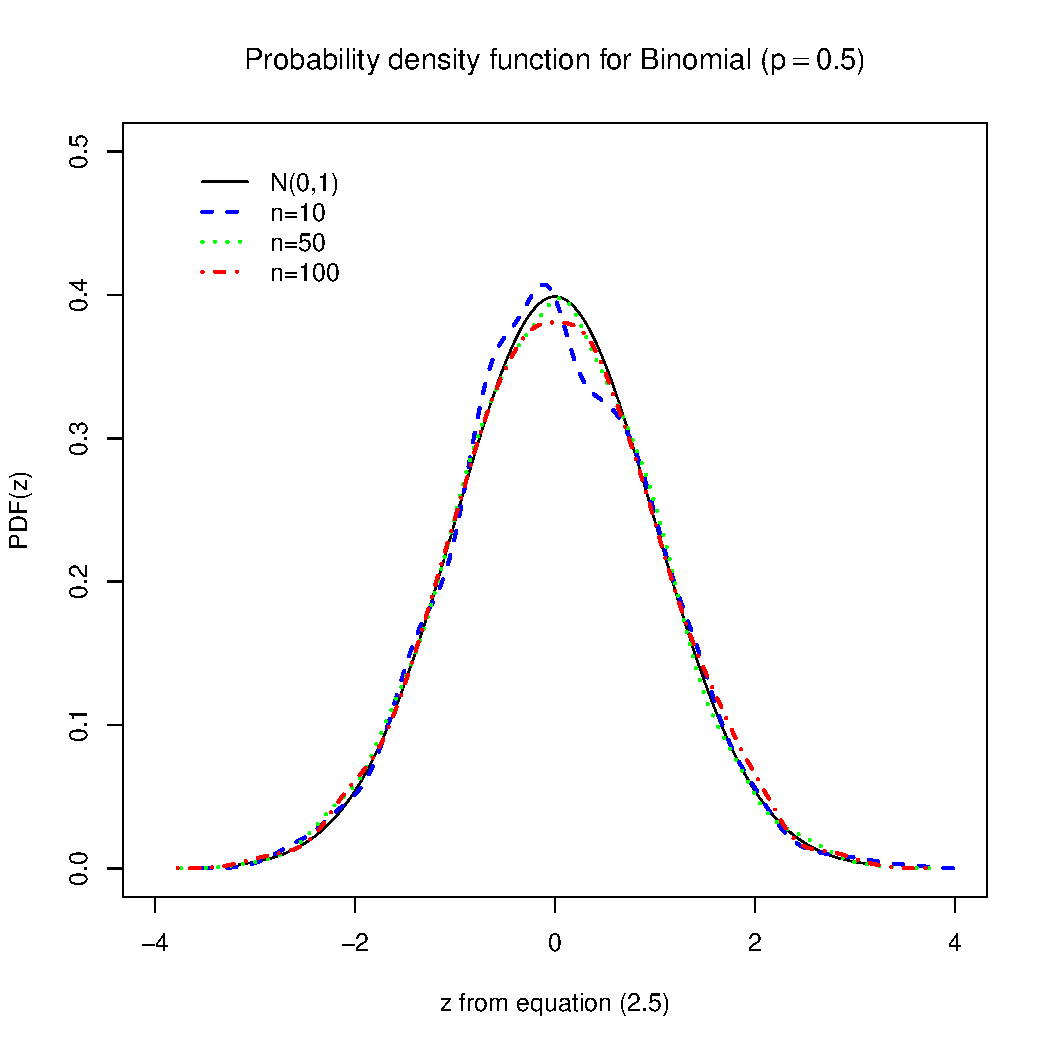
\includegraphics[width=0.49\textwidth]{Figures/binomial_PDF.pdf} \hfill
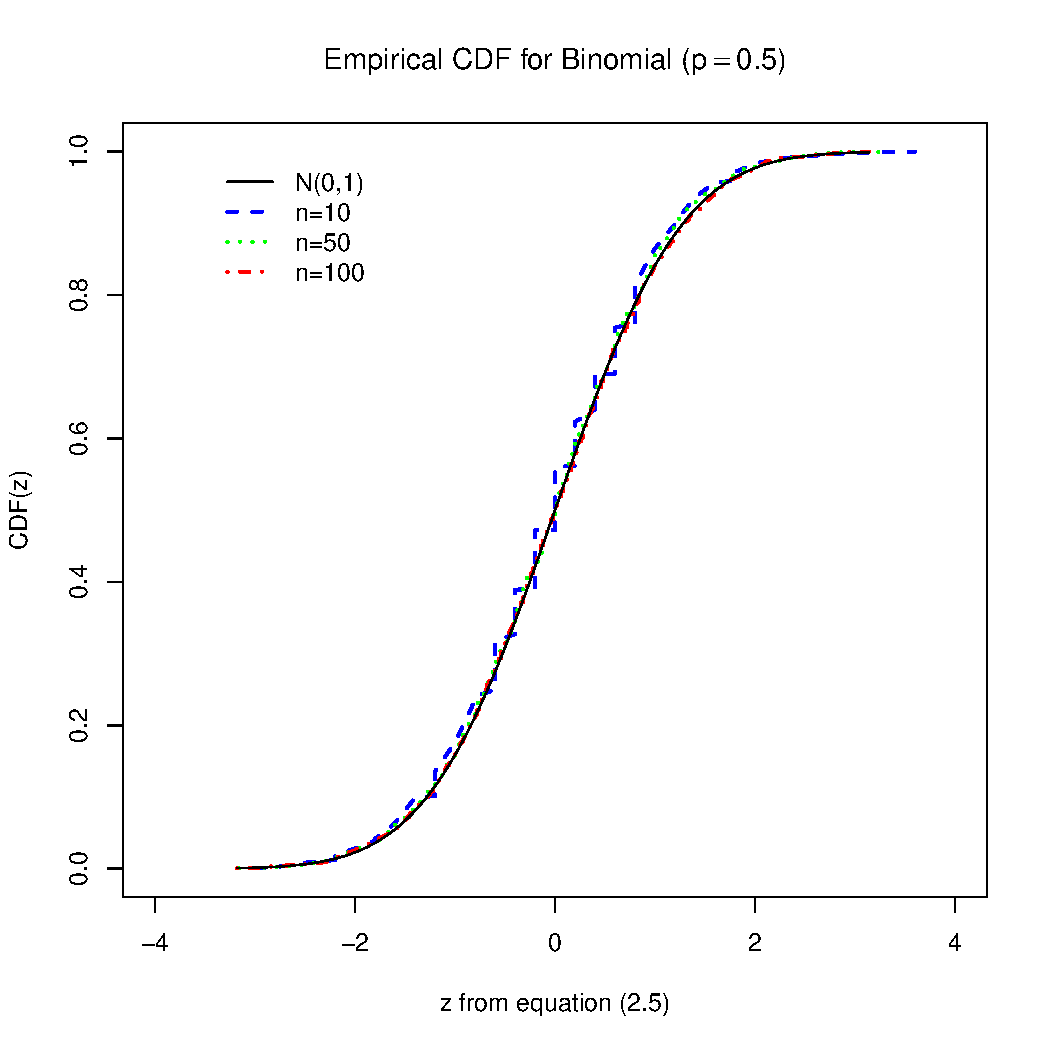
\includegraphics[width=0.49\textwidth]{Figures/binomial_CDF.pdf}\\
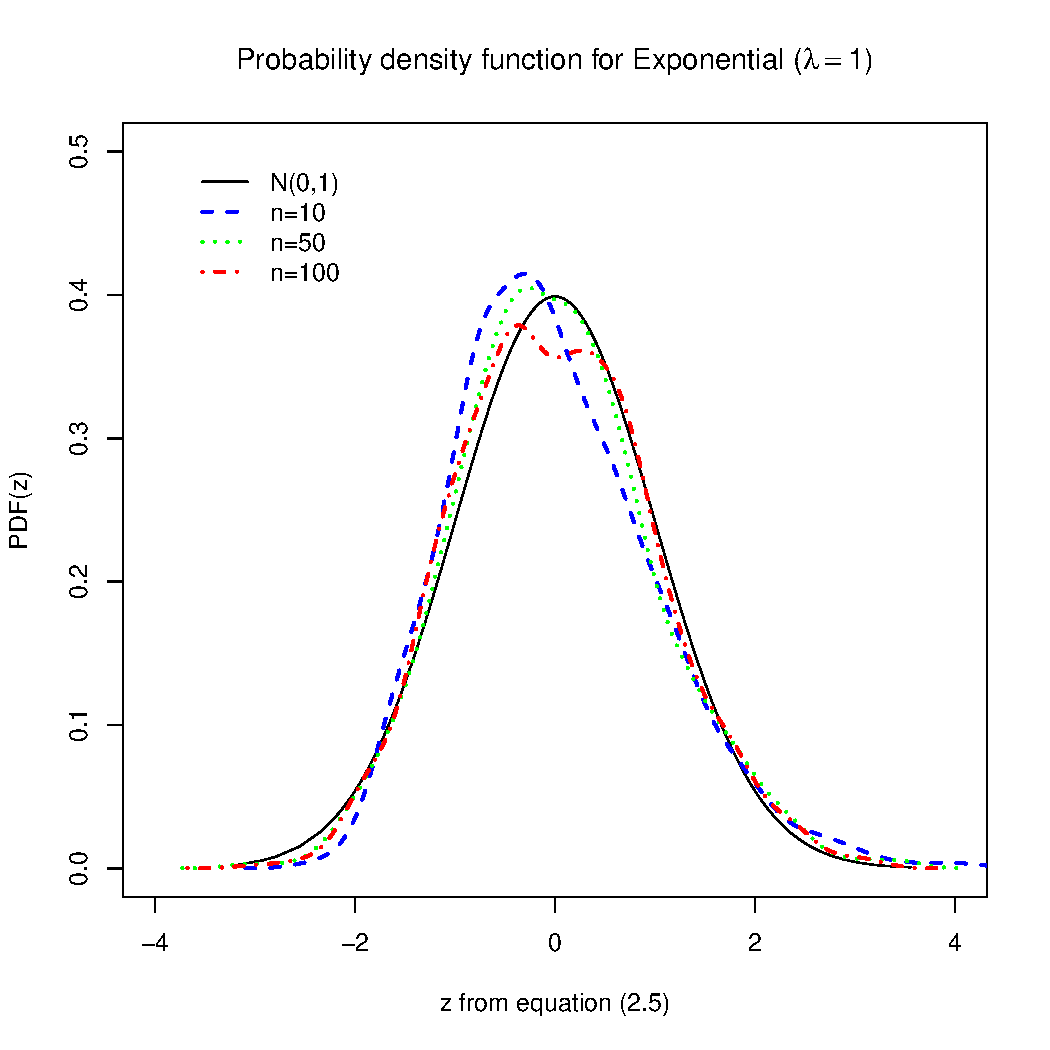
\includegraphics[width=0.49\textwidth]{Figures/expon_PDF.pdf} \hfill
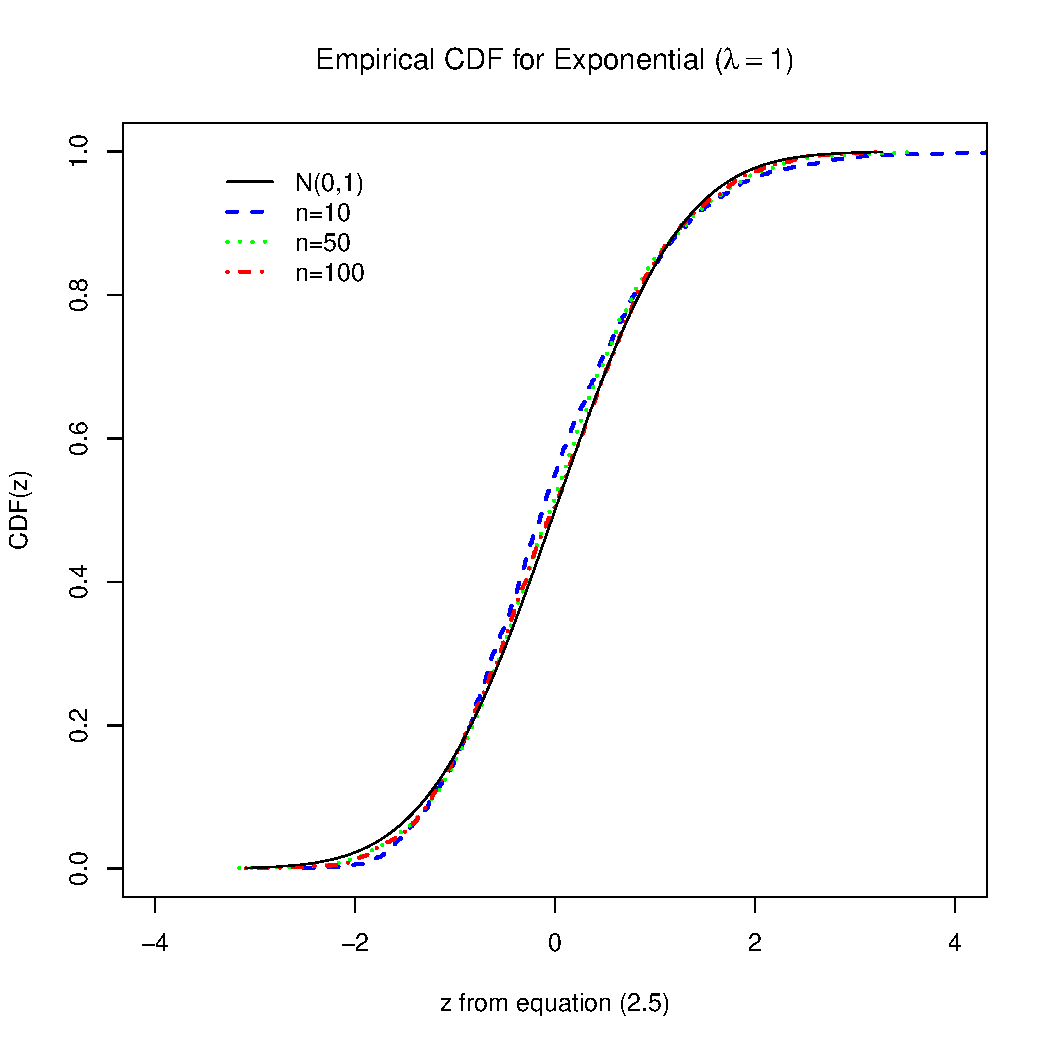
\includegraphics[width=0.49\textwidth]{Figures/expon_CDF.pdf}\\
\caption{Normal approximation for binomial and exponential distribution}\label{fig.CLT1}
\end{figure}

\begin{figure}[htp]
\centering
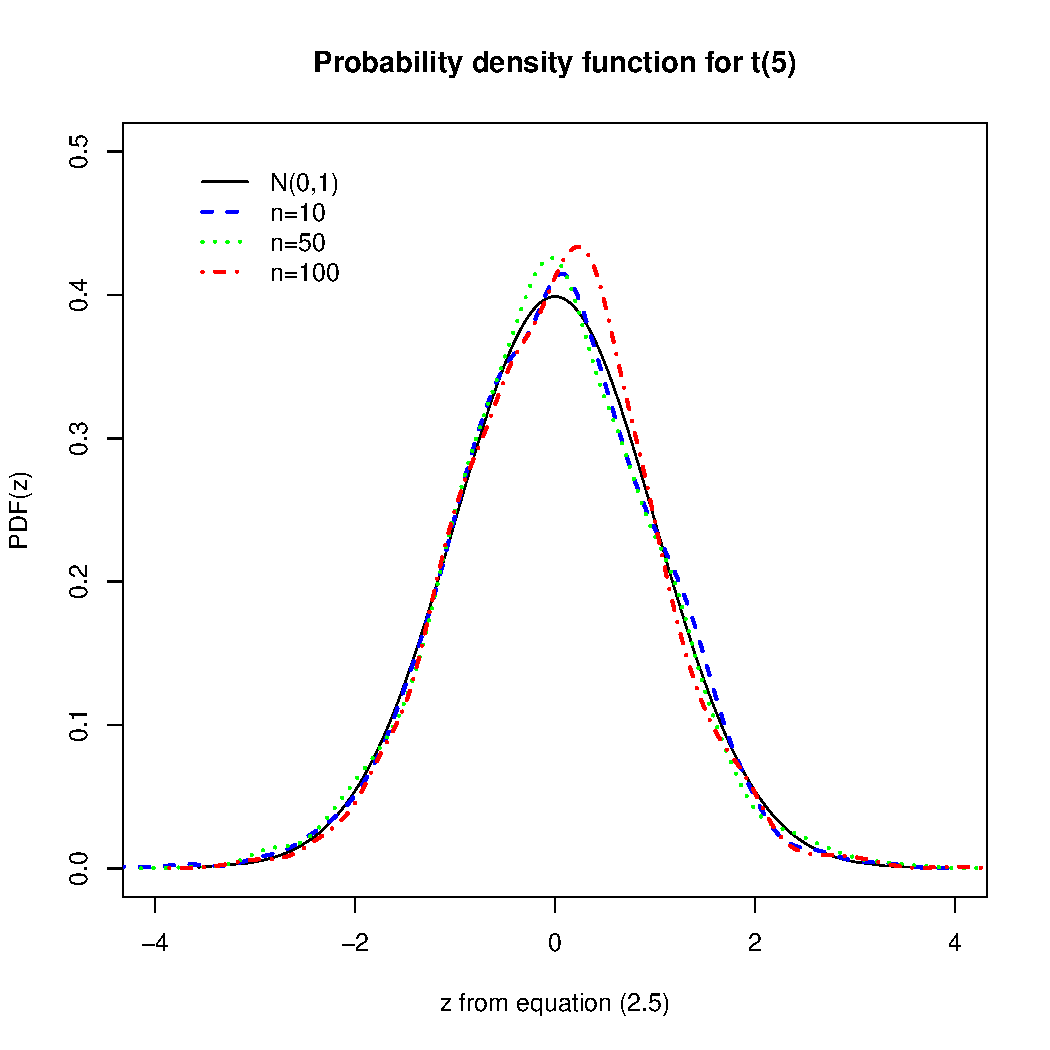
\includegraphics[width=0.49\textwidth]{Figures/t_PDF.pdf} \hfill
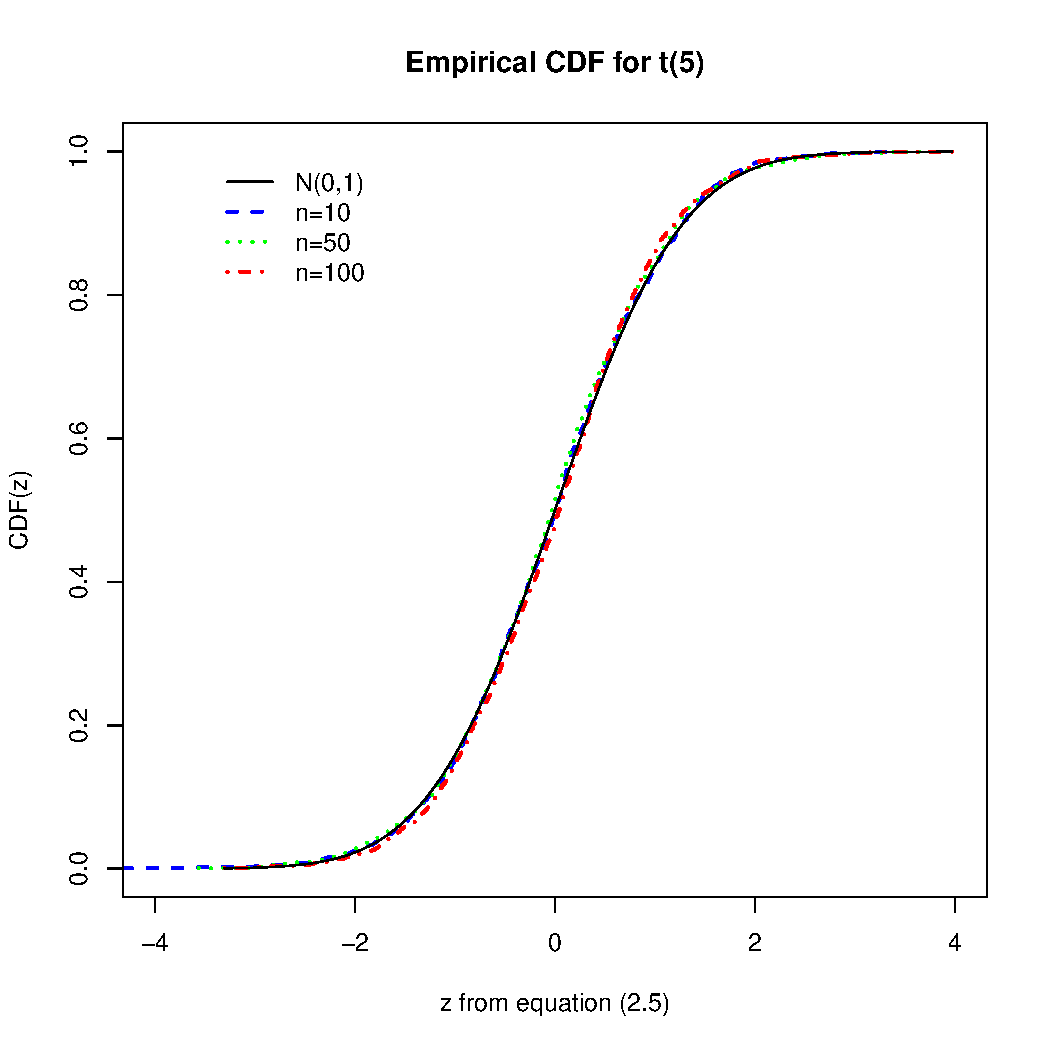
\includegraphics[width=0.49\textwidth]{Figures/t_CDF.pdf}\\
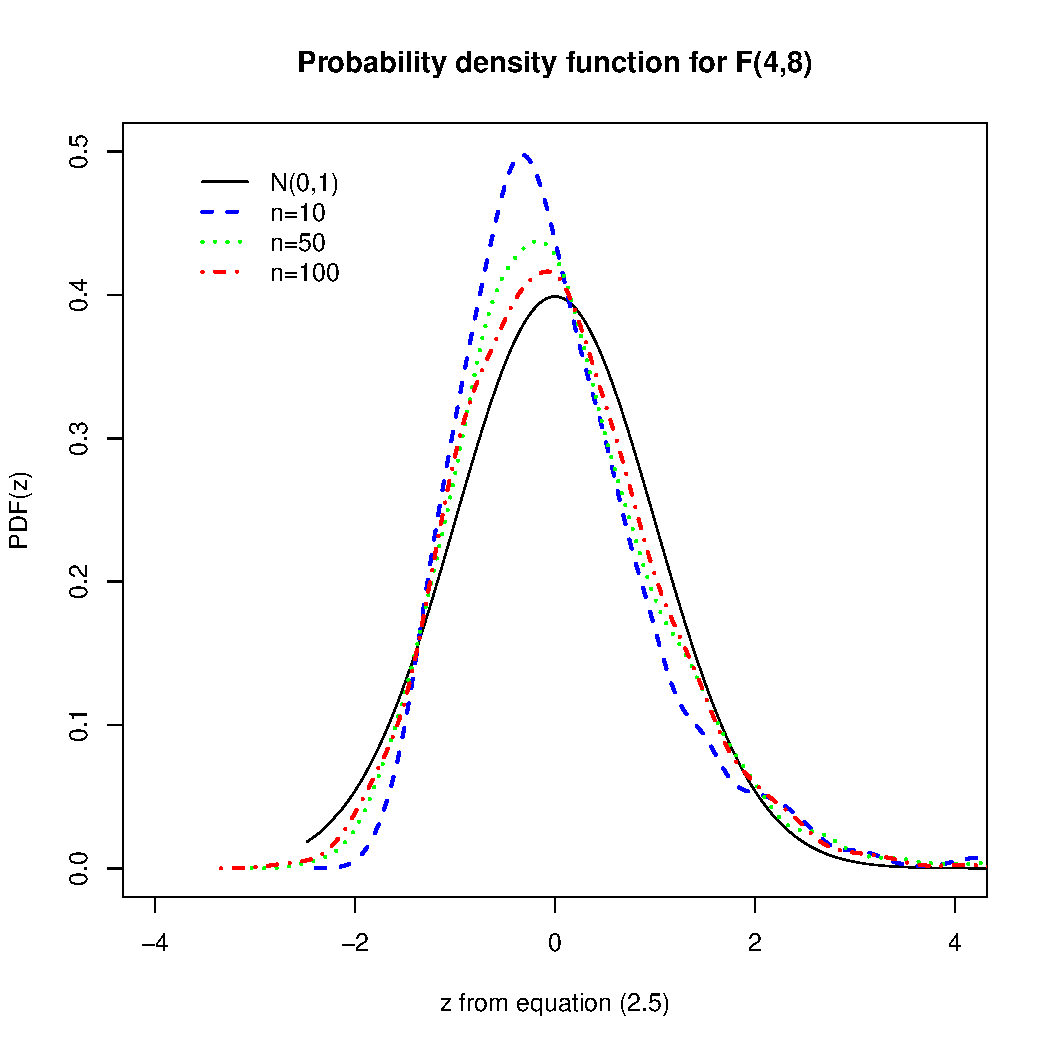
\includegraphics[width=0.49\textwidth]{Figures/f_PDF.pdf} \hfill
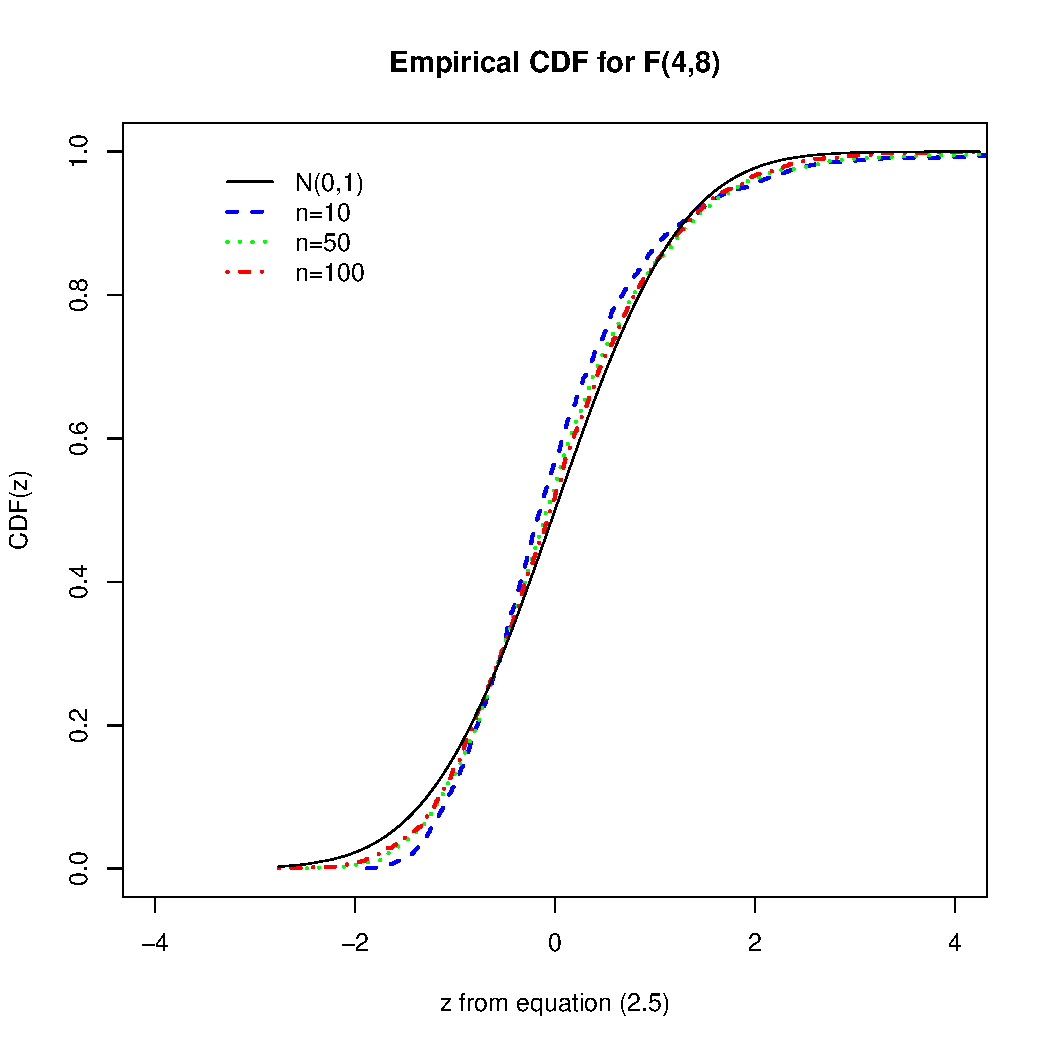
\includegraphics[width=0.49\textwidth]{Figures/f_CDF.pdf}\\
\caption{Normal approximation for $t$- and $F$-distribution}\label{fig.CLT2}
\end{figure}

\begin{figure}[htp]
\centering
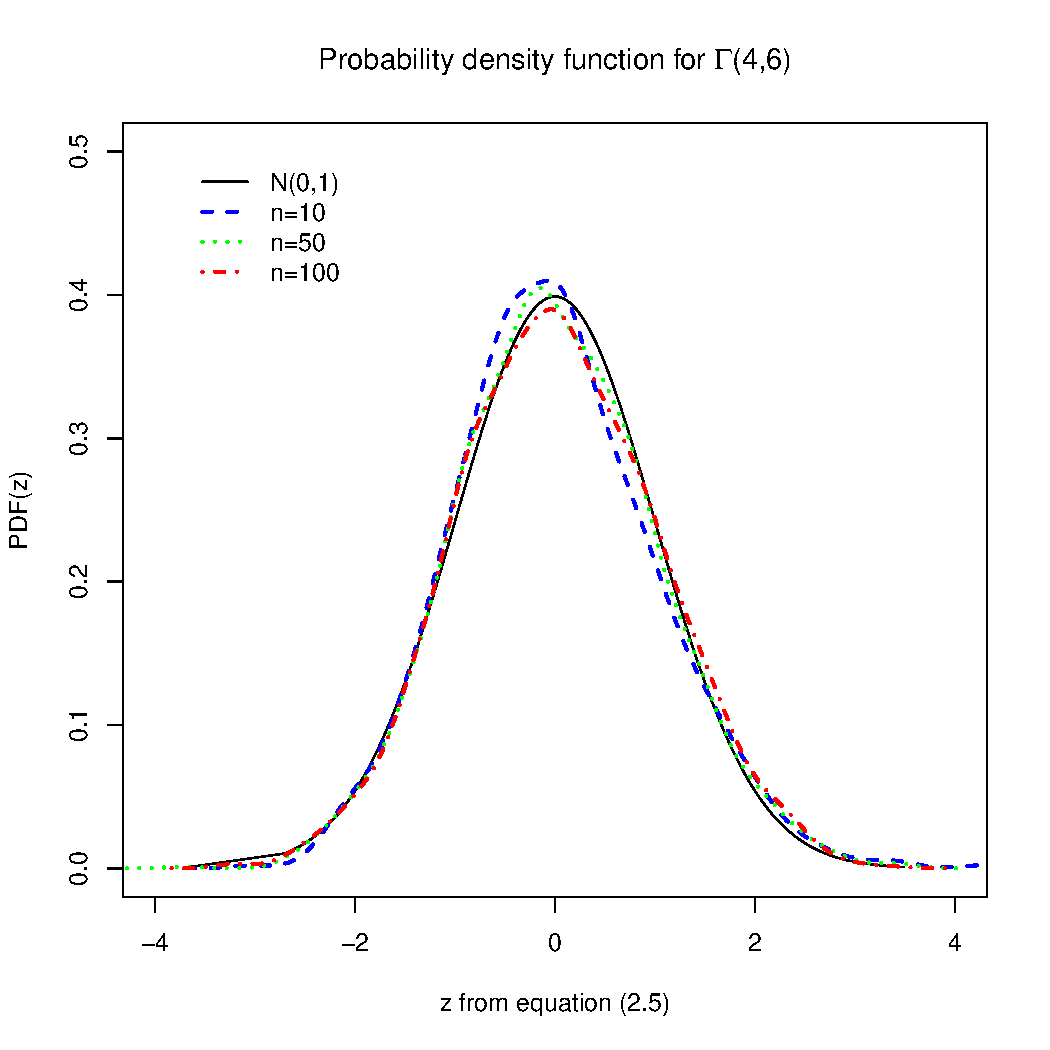
\includegraphics[width=0.49\textwidth]{Figures/gamma_PDF.pdf} \hfill
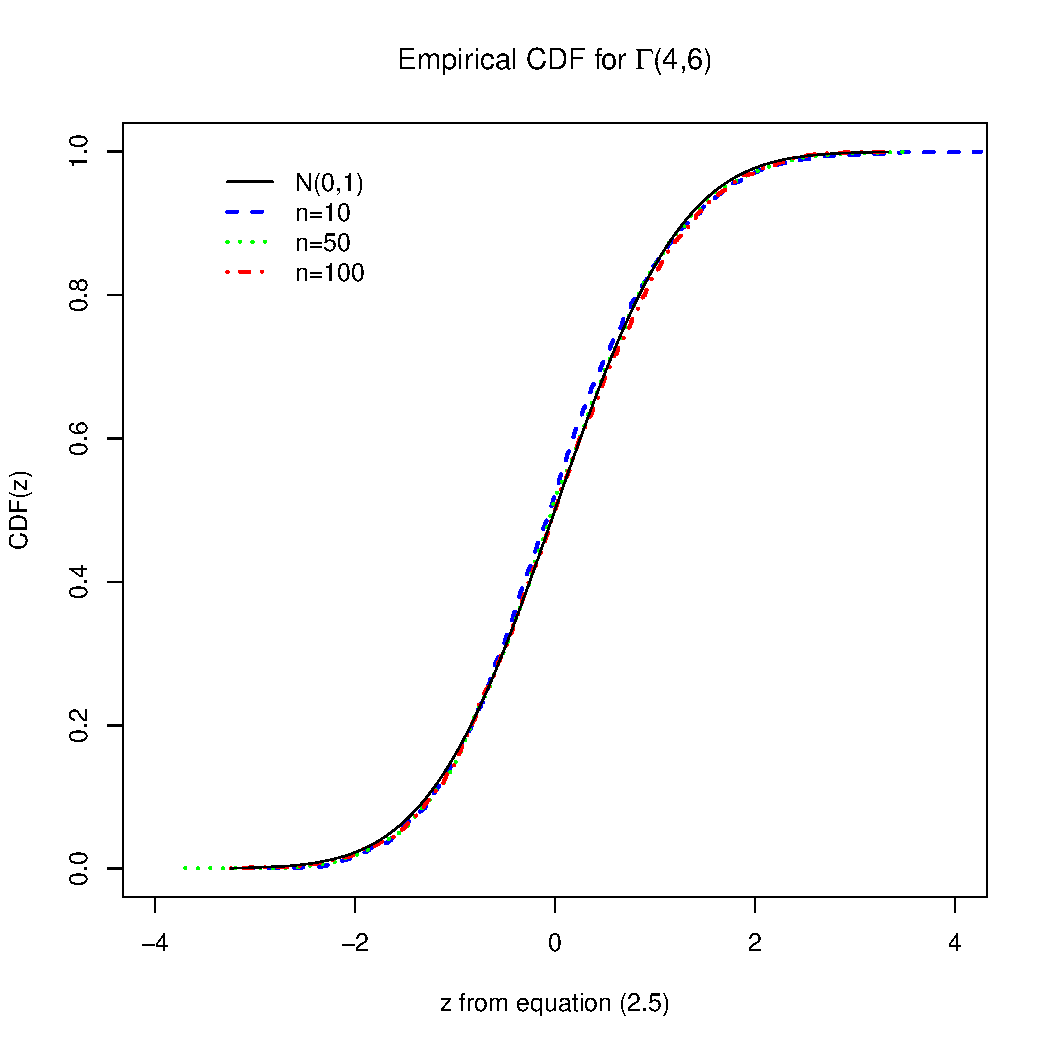
\includegraphics[width=0.49\textwidth]{Figures/gamma_CDF.pdf}\\
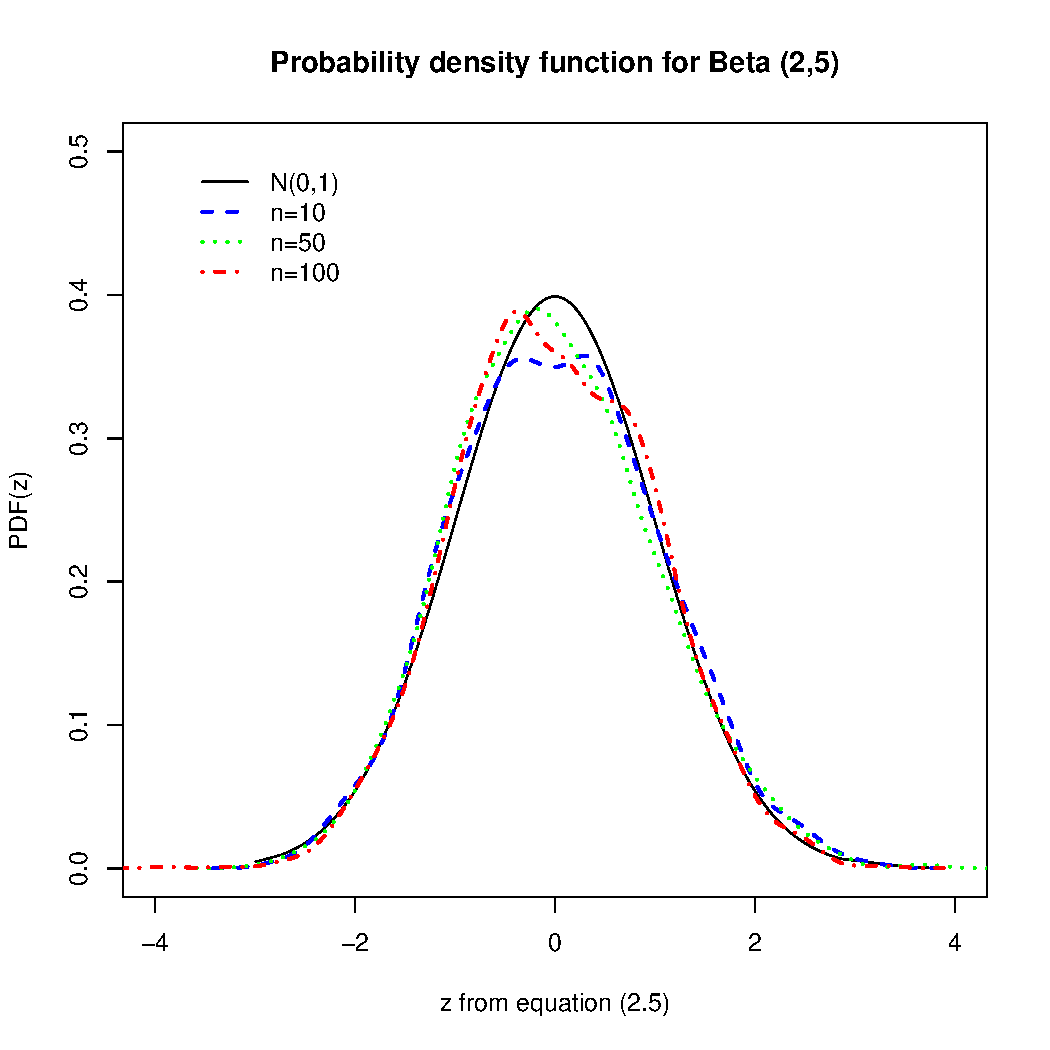
\includegraphics[width=0.49\textwidth]{Figures/beta_PDF.pdf} \hfill
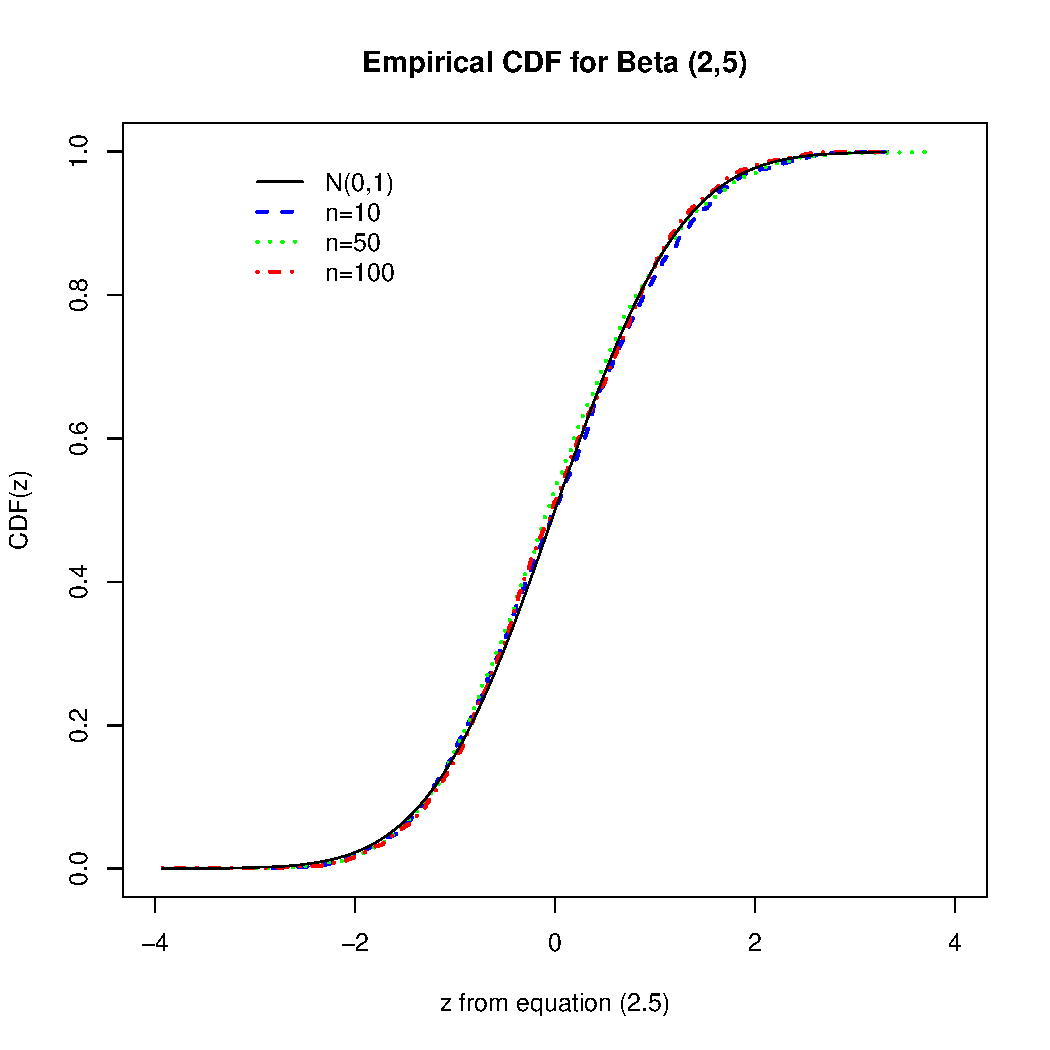
\includegraphics[width=0.49\textwidth]{Figures/beta_CDF.pdf}\\
\caption{Normal approximation for $\Gamma$- and Beta distribution}\label{fig.CLT3}
\end{figure}

Overall, this exercise demonstrates how powerful the CLT really is; for all six different distributions, $1/\sqrt(n)$ times the sum of $n$ centered random variables approximately follows a normal distribution even at $n$ as small as 10. Figures~\ref{fig.CLT1} to figure~\ref{fig.CLT3} show the empirical distribution functions for the six distributions.

\begin{itemize}
\item[\emph{Binomial}] The approximation to the standard normal distribution increases dramatically at $n=50$ as the step function is still visible at $n=10$.
\item[\emph{Exponential}] CLT takes effect visibly at $n=50$
\item[\emph{t}] Even at $n=10$, the centered random variables from the $t$-distribution approximate N(0,1) well. It is hardly surprising since the two distributions are very similar except that the t-distribution displays wider tails.
\item[\emph{F}] Centering for random variables from the $F$-distribution approximates the normal distribution only at comparatively large $n$, with the CLT fully taking effect at $n=100$
\item[\emph{Gamma}] Centered random variables from the $\Gamma$-distribution approximate N(0,1) reasonably well at the smallest $n$ with the CLT kicking more reliably at $n=50$.
\item[\emph{Beta}] Even at $n=10$, the centered random variables from the Beta-distribution approximate N(0,1) well. However for this distribution, the CLT-threshold seems to depend significantly on the random seed and fluctuated in different simulations between $n=10$ and $n=50$.
\end{itemize}

In addition to discovering that the CLT becomes effective at relatively small $n$ for a variety of distributions, this exercise demonstrates the impact of the variance on the centering process. The $\chi^{2}(m)$ distribution approaches the N($m,2m$) as $m$ becomes large and its variance is $2m$.

\begin{figure}[htp]
\centering
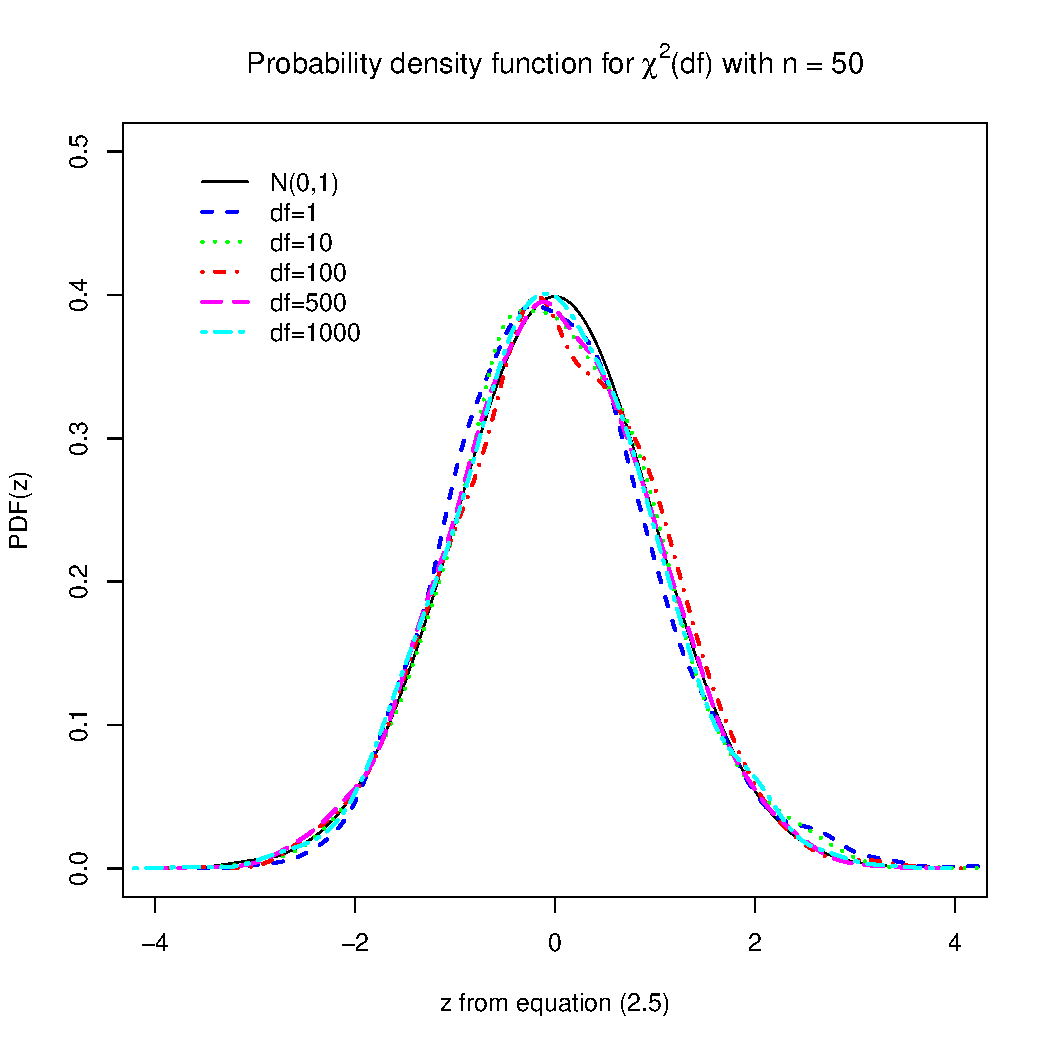
\includegraphics[width=0.75\textwidth]{Figures/chi1_PDF.pdf}
\caption{Normal approximation for $\chi^{2}$-distribution}\label{fig.CLT5}
\end{figure}

The different panels of figure~\ref{fig.CLT6} demonstrate that the \emph{variance} and \emph{sample size} work as \emph{substitutes} in the centering process; a higher variance requires a smaller sample size in order for the $\chi^{2}(m)$-distribution to approximate the standard normal distribution. This largely due to the fact that centering is achieved by subtracting the mean and dividing by the standard deviation. A large variance implies a large denominator which in turn implies that a smaller number of observations are required for the distribution to be asymptotically distributed as N(0,1).

\begin{figure}[htp]
\centering
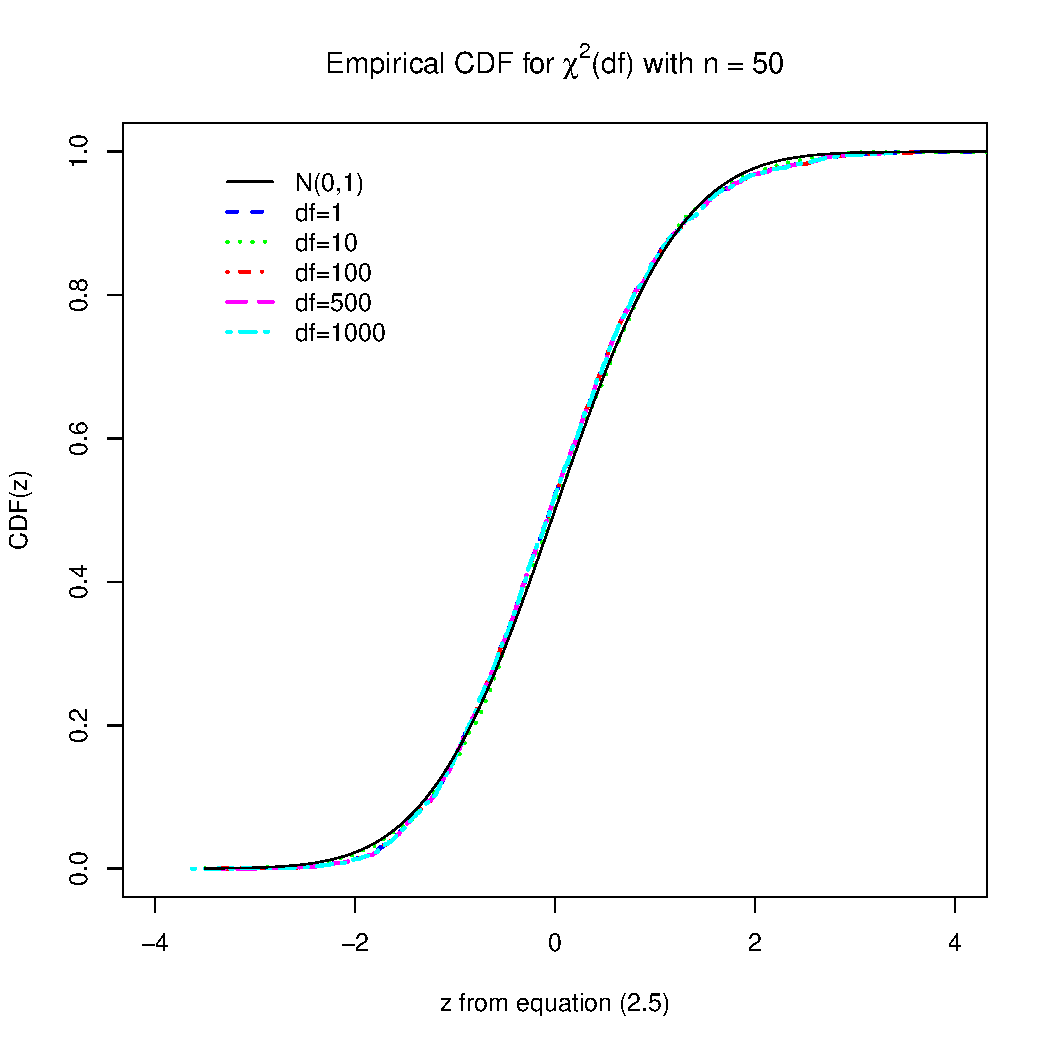
\includegraphics[width=0.49\textwidth]{Figures/chi2_CDF.pdf} \hfill
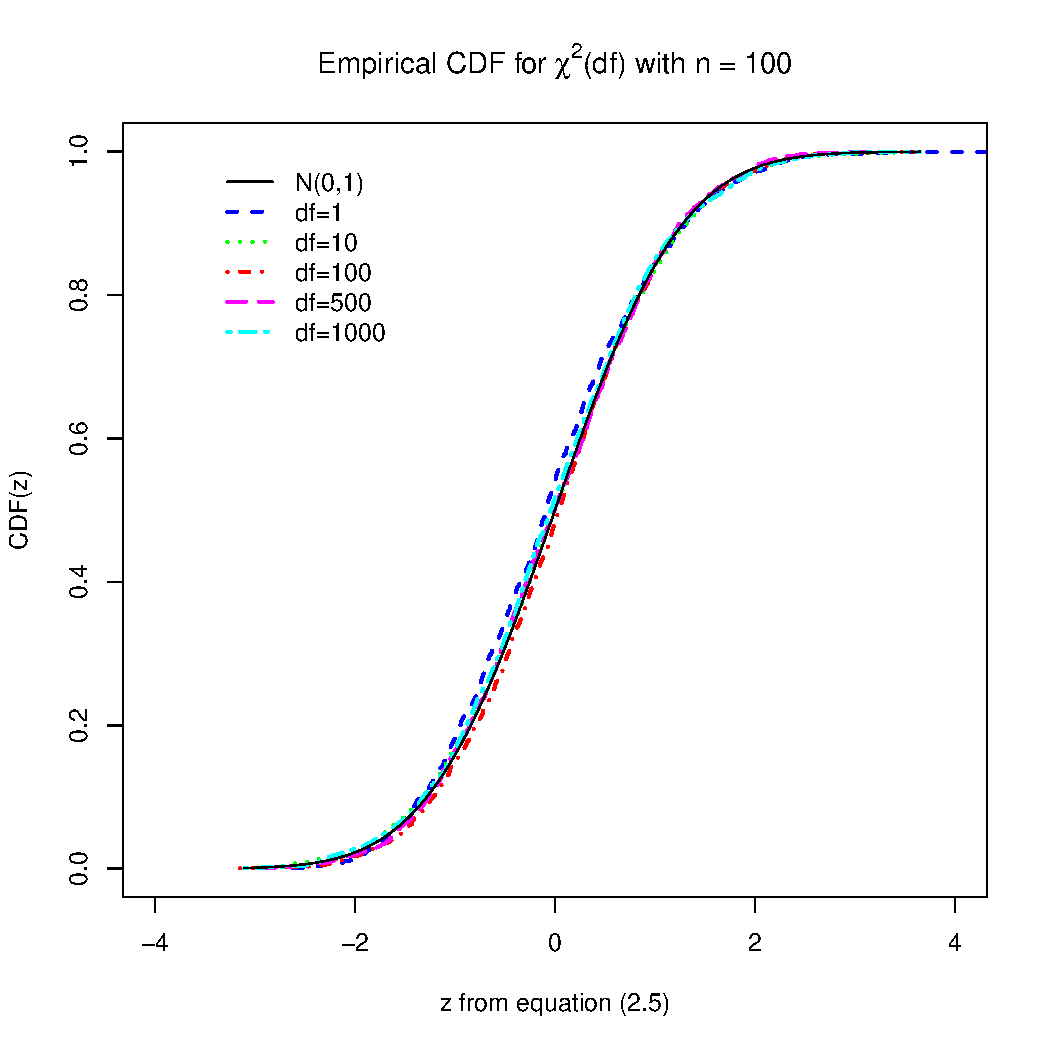
\includegraphics[width=0.49\textwidth]{Figures/chi3_CDF.pdf}\\
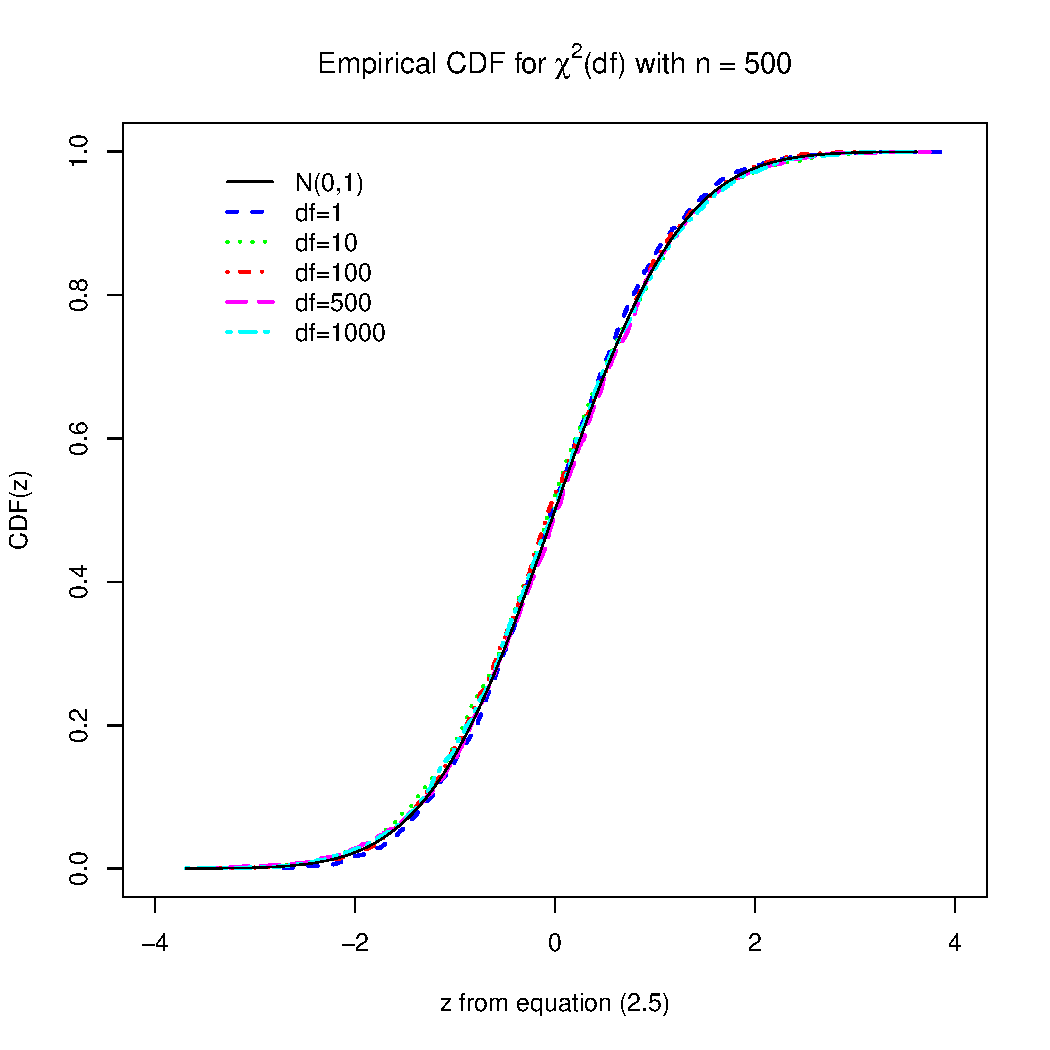
\includegraphics[width=0.49\textwidth]{Figures/chi4_CDF.pdf} \hfill
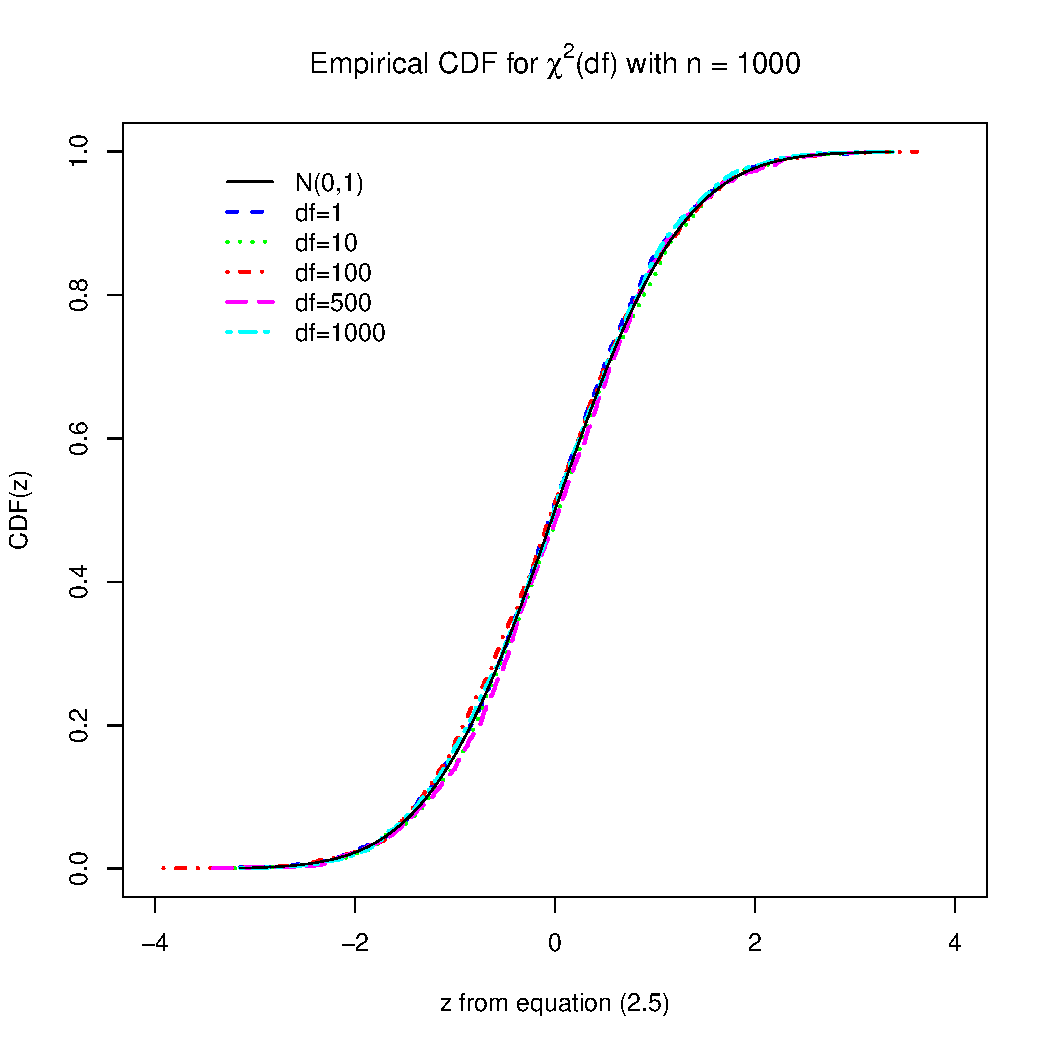
\includegraphics[width=0.49\textwidth]{Figures/chi5_CDF.pdf}\\
\caption{Variance impact and CLT for $\chi^{2}$-distribution}\label{fig.CLT6}
\end{figure}


\section{Matrix algebra}\label{chap_Review:Matrix}

\renewcommand\bibname{Further reading}
\begin{subappendices}
\bibliographystyle{econometrica}
\bibliography{Literature/OverLord}
\IfFileExists{Literature/Review.bbl}{\chapter{Review}\label{chap_Review}
\section{Preliminaries}\label{chap_Review:Prelim}
``Probability approach in econometrics'' by Trygve \citet{Haavelmo1944} stands at the beginning of a paradigm shift in statistical thinking; the \emph{classical} interpretation of statistics is giving way to the \emph{frequentist} interpretation. Under the classical interpretation, probabilities are linked to the principle of indifference and statistical events are governed by natural symmetry (e.g. coin tosses, die etc.) This constraining set-up of what gives rise to probabilities is one of the key problems of the classical view. 

Under the frequentist interpretation on the other hand, probabilities of events are linked to the frequency with which a given event is observed. This implies that

$$P(x)= \lim\limits_{n_{t} \rightarrow \infty} \frac{n_{x}}{n_{t}},$$ 

where $n_{x}$ is the number of observed trials and $n_{t}$ is the total number of trials. This probabilistic approach to statistics, which includes Bayesian statistics\index{Bayesian statistics}, represents the world in terms of ``degrees of belief'' (Bayesian priors).

More formally, Bayes' Theorem is expressed as the conditional probability of occurence A given B such that $$P(A|B) = \frac{P(B|A)P(A)}{P(B)}.$$\index{Bayes' Theorem|see{Bayesian statistics}}


\section{Statistics and probability theory}\label{chap_Review:Stats}
\subsection{Types of random variables}
A random variable, usually written as $X$, is a variable whose possible values are numerical outcomes of a random phenomenon. A random variable $X$  is a (real) number with the following characteristics:

\begin{inparaenum}[\itshape a\upshape)]
\item the value of $X$ is unknown;
\item the possible values $X$ can take are known; the set of such values is called support and denoted by $\bm{\mathcal{S}}_{X}$;
\item if $\bm{\mathcal{A}}$  is a subset of the set of real numbers $\mathbb{R}$  (i.e. $\bm{\mathcal{A}}\subseteq \mathbb{R}$), we know the probability that $X$ belongs to $\bm{\mathcal{A}}$ which is denoted by $P(X\in\bm{\mathcal{A}})$.
\item If (and when) the value $x$ of $X$  becomes known, such that $x=X$, $x$ is then referred to as the realization of $X$. Hence, the support $\bm{\mathcal{S}}_{X}$  is the set of all possible realizations of $X$.
\end{inparaenum}

Random variables generally fall into two categories, discrete and continuous:

\begin{itemize}
\item Discrete random variables\index{random variable!discrete}: Takes on only a countable number of distinct values such as $0,1,2,3,4 \ldots$ Discrete random variables are usually (but not necessarily) counts. If a random variable can take only a finite number of distinct values, then it must be discrete.
\item Continuous random variables\index{random variable!continuous}: Takes an infinite number of possible values. Continuous random variables are usually measurements. Examples include height, weight, the amount of sugar in an orange, the time required to run a mile.
\end{itemize}

In addition to distinguishing between discrete and continuous random variables, we can also categorise random variables into \emph{qualitative} variables or \emph{quantitative} variables. Qualitative\index{qualitative variable|see{random variable}} or categorical variables are either nominal, ordinal or dichotomous. 

\begin{itemize}
\item Nominal variables: \index{random variable!nominal}\index{categorical variable|see{random variable}} A variable for mutually exclusive, but not ordered categories such as, for example, your study might compare five different types of suburbs (inner-ring suburbs, commuter suburb, sitcom suburb, high-income suburb, minority suburb). 
\item An ordinal variable\index{random variable!ordinal} is a random variable where the order matters but not the difference between values. For example, quality of life rankings might express how nice a place is on a scale of 1 to 10. A score of 7 means a nicer place that a score of 5, and that is more than a score of 3. But the difference between the 7 and the 5 may not be the same as that between 5 and 3. The values simply express an order. 
\end{itemize}

Quantitative variables\index{quantitative variable|see{random variable}} are either interval variables where differentiation or transformation preserves the units (such as in the case of temperature measurements in C, F) or ratio variables where a value of 0 means that nothing of that variable is present. Thus temperature measured in Kelvin or height, for example, are ratio variables.

\begin{itemize}
\item An interval variable\index{random variable!interval} is a measurement where the difference between two values is meaningful. The difference between a temperature of 100 degrees and 90 degrees is the same difference as between 90 degrees and 80 degrees. 
\item When working with ratio variables\index{random variable!ratio}, you can look at the ratio of two measurements. A weight of 4 grams is twice a weight of 2 grams, because weight is a ratio variable. A temperature of 100 degrees Celsius is not twice as hot as 50 degrees C, because temperature C is not a ratio variable. Similarly, a pH of 3 is not twice as acidic as a pH of 6, because pH is an interval variable and not a ratio variable. 
\end{itemize}

\begin{table}[htp] 
\centering
\caption{Basic statistical operations by variable type}
\footnotesize
\begin{tabular}{lcccc}\label{tbl_Vars}
\\ \hline
\hline
&\multicolumn{4}{c}{\emph{Random variable type}}\\
\emph{Operation}&Nominal&Ordinal&Ratio&Interval\\
\cline{2-5}
Frequency distribution&Yes&Yes&Yes&Yes\\
Median and percentiles&No&Yes&Yes&Yes\\
Addition/subtraction&No&No&Yes&Yes\\
Mean, standard deviation, standard error of the mean&No&No&Yes&Yes\\
Ratio/coefficient of variation&No&No&No&Yes\\
\hline
\hline \\
\normalsize
\end{tabular}
\end{table}


\subsection{Expectations}
\subsubsection{Expectation of a discrete random variable}
\begin{eqnarray}
\mathbb{E}(X) &=& x_{1}p_{1} + x_{2}p_{2} + x_{3}p_{3} +\ldots + x_{n}p_{n}\nonumber \\
&=& \sum^{n}_{i=1}x_{i}p_{i}
\end{eqnarray}

Recall that in a finite sample, $\mathbb{E}(X)$ denotes the sample mean and the sum of all probabilities must be equal to one, i.e. $\sum_{i}p_{i}=1$.

\paragraph{Example} Consider the following gamble where an unbiased coin with heads ($H$) and tails ($T$) is tossed $n$ times until tails ($T$) appears. If $T$ shows up at the $n$-th toss, the payoff is $\$2^{n-1}$. How much would you be willing to put up as a wager to participate in this game?

\begin{eqnarray*}
\mathbb{E}(X) &=& \$2^{0}\cdot\frac{1}{2} + \$2^{1}\cdot\frac{1}{2}\cdot\frac{1}{2} + \$2^{2}\cdot\frac{1}{2}\cdot\frac{1}{2}\cdot\frac{1}{2} + \ldots \\
&=& \$1\cdot\frac{1}{2} + \$2\cdot\frac{1}{4} + \$4\cdot\frac{1}{8} + \ldots\\
&=& \sum^{\infty}_{i=1}\$ 0.5 = \$\infty
\end{eqnarray*}

This is the \emph{St. Petersburg paradox}\index{St. Petersburg paradox} famously defined and described by Daniel Bernoulli\index{Bernoulli, Daniel} (Swiss mathematician (1700--1782), father of modern fluid dynamics) to illustrate the failure of expected value principle (as opposed to expected utility) in decision theory under uncertainty. Thus the expected payout value of a St. Petersburg game is an infinite amount, yet clearly the willingness to pay (WTP)\index{WTP|see{willingness to pay}}\index{willingness to pay} to participate in such a game must be (much) less than its expected value. The classical resolution of the paradox thus involves the explicit introduction of a utility function\index{utility}, an expected utility hypothesis, and the presumption of diminishing marginal utility of money. This implies $\mathbb{E}(U) < \mathbb{E}(X)$.

\paragraph{Example} What is the expected value of throwing a single die (or a pair of dice)?

\begin{eqnarray*}
\mathbb{E}(X) = \frac{1}{6}\cdot 1 + \frac{1}{6}\cdot 2 + \frac{1}{6}\cdot 3 + \ldots + \frac{1}{6}\cdot 6 = 3.5
\end{eqnarray*}

Thus the sample mean $\mu_{X} = 3.5$ and analogously, for a pair of dice, $\mu_{X} = 7$. A table with the bivariate probabilities is shown in table~\ref{tbl_Dice} below:


\begin{table}[htp] 
\centering
\caption{Bivariate probabilities for a pair of dice and expected value of $X$}
\footnotesize
\bigskip
\begin{tabular}{lll|lll}\label{tbl_Dice}
\\ \hline
\hline
$X$&$p$&$Xp$&$X$&$p$&$Xp$\\
\hline
$x_{1}$ & $p_{1}$ & $x_{1}p_{1}$ & 2 & 1/36 & 2/36\\
$x_{2}$ & $p_{2}$ & $x_{2}p_{2}$ & 3 & 2/36 & 6/36\\
$x_{3}$ & $p_{3}$ & $x_{3}p_{3}$ & 4 & 3/36 & 12/36\\
$\ldots$ & $\ldots$ & $\ldots$ & 5 & 4/36 & 20/36\\
$\ldots$ & $\ldots$ & $\ldots$ & 6 & 5/36 & 30/36\\
$\ldots$ & $\ldots$ & $\ldots$ & 7 & 6/36 & 42/36\\
$\ldots$ & $\ldots$ & $\ldots$ & 8 & 5/36 & 40/36\\
$\ldots$ & $\ldots$ & $\ldots$ & 9 & 4/36 & 36/36\\
$\ldots$ & $\ldots$ & $\ldots$ & 10 & 3/36 & 30/36\\
$\ldots$ & $\ldots$ & $\ldots$ & 11 & 2/36 & 22/36\\
$x_{n}$ & $p_{n}$ & $x_{n}p_{n}$ & 12 & 1/36 & 6/36\\

\hline
\multicolumn{3}{l}{Total: $\mathbb{E}(X)=\sum^{n}_{i=1}x_{i}p_{i}$}&&\multicolumn{2}{r}{252/36 = 7}\\
\hline \\
\normalsize
\end{tabular}
\end{table}


\subsection{Expectations rules}
\begin{enumerate}
\item $\mathbb{E}[X + Y + Z] = \mathbb{E}(X) + \mathbb{E}(Y) + \mathbb{E}(Z);$
\item $\mathbb{E}[bX] = b\mathbb{E}(X);$
\item $\mathbb{E}[b] = b$
\end{enumerate}

\paragraph{Example} Different rules can be combined, e.g. $\mathbb{E}[a + bX] = a + b\mathbb{E}(X)$. Let a normally distributed random variable $V$ can have any mean $\mu$ and any positive variance $\sigma^{2}$. Such a random variable is said to follow the $\mathcal{N}(\mu, \sigma^{2})$ distribution. A standard normal variable therefore has the $\mathcal{N}(0, 1)$ distribution.

Suppose that $V$ has the standard normal distribution. What are the corresponding mean $\mu$ and variance $\sigma^{2}$ of a new random variable $Z \equiv \mu + \sigma V$? For the mean, we use the fact that $\mathbb{E}\left[V\right]=0$ which yields

\begin{eqnarray*}
\mathbb{E}\left[Z\right] &=& \mathbb{E}\left[\mu + \sigma V\right] = \mathbb{E}\left[\mu\right] + \mathbb{E}\left[\sigma V\right] = \mu + \sigma\mathbb{E}\left[V\right]\\
&=& \mu.
\end{eqnarray*}

Similarly, when deriving the variance, recall that $\text{var}(V)=\mathbb{E}\left[V^{2}\right]=1$ such that

\begin{eqnarray*}
    \mathbb{E}\left[(Z-E\left[Z\right])^{2}\right] &=& \mathbb{E}\left[Z^{2}-2Z\mathbb{E}\left[Z\right]+ (\mathbb{E}\left[Z\right])^{2}\right]= \mathbb{E}\left[Z^{2} -2Z\mu + \mu^{2}\right]\\
    &=& \mathbb{E}\left[Z^{2}\right] -2\mu\mathbb{E}\left[Z\right] + \mathbb{E}\left[\mu^{2}\right]= \mathbb{E}\left[Z^{2}\right] -2\mu^{2} + \mu^{2}\\
    &=& \mathbb{E}\left[(\mu^{2}+ 2\mu\sigma V + \sigma^{2}V^{2})\right] -\mu^{2} \\
    &=& \mu^{2} + 2\mu\sigma \mathbb{E}\left[V\right] +\sigma^{2}\mathbb{E}\left[V^{2}\right] -\mu^{2} =  \\
    &=& \sigma^{2}.
    \end{eqnarray*}


\subsubsection{Variance of a discrete random variable}
\begin{eqnarray}
\textrm{Var}(X) = \sigma^{2}_{X} &=& \mathbb{E}[(X-\mu_{X})^{2}]\nonumber \\
&=& (x_{1} - \mu_{X})^{2}p_{1} + (x_{2} - \mu_{X})^{2}p_{2} + \ldots + (x_{n} - \mu_{X})^{2}p_{n} \nonumber\\
&=& \sum^{n}_{i=1}(x_{i} - \mu_{X})^{2}p_{i}
\end{eqnarray}

Derivation of alternative expression for the variance:

\begin{eqnarray}
\textrm{Var}(X) = \sigma^{2}_{X} &=& \mathbb{E}[(X-\mu_{X})^{2}]\nonumber \\
&=& \mathbb{E}[(X-\mu_{X})((X-\mu_{X})] \nonumber\\
&=& \mathbb{E}[X^{2}-2\mu_{X}X + \mu_{X}^{2}] \nonumber\\
&=& \mathbb{E}[X^{2}] -\mathbb{E}[2\mu_{X}X] + \mathbb{E}[\mu_{X}^{2}] \nonumber\\
&=& \mathbb{E}[X^{2}] -2\mu_{X}\mathbb{E}[X] + \mu_{X}^{2} \nonumber\\
&=& \mathbb{E}[X^{2}] -2\mu_{X}^{2} + \mu_{X}^{2} = \mathbb{E}[X^{2}] - \mu_{X}^{2}
\end{eqnarray}

\subsubsection{Fixed and random components of variables}
Let the random variable $X$ be decomposed into two parts, namely a constant mean $\mu_{X}$ and a variable component $u$. Think of $u$ as measurement error or a stochastic disturbance term with $\mathbb{E}(u)= \mathbb{E}(X-\mu_{X}) = \mathbb{E}(X) -\mu_{X}= 0$.

Because all variation in $X$ is due to $u$, the variance of $X$, $\sigma^{2}_{X}$, is identical to the variance of the disturbance term, $\sigma_{u}$. More formally, we can write

\begin{eqnarray*}
\sigma^{2}_{X}&=& \mathbb{E}[(X-\mu_{X})^{2}] = \mathbb{E}(u^{2})\\
\sigma^{2}_{u}&=& \mathbb{E}[(u-\mu_{u})^{2}] = \mathbb{E}(u^{2}).
\end{eqnarray*}

\section{Probability distributions}
All random variables (discrete and continuous) have a probability density function (PDF)\index{PDF|see{density function}}\index{density function!probability} and a cumulative density function (CDF)\index{CDF|see{density function}}\index{density function!cumulative}. These are functions that give the probability that the random variable $X$ is less than or equal to $x$, for every value $x$. For a discrete random variable, the cumulative distribution function is found by summing up the probabilities.


\begin{figure}[htp]
\caption{Probability density function with $f(x)\equiv F'(x)$ }\label{fig_PDF}
\begin{center}
\includegraphics[width=0.7\textwidth]{"Figures/PDFjc"}
\end{center}
\footnotesize
\end{figure}


\begin{figure}[htp]
\caption{Cumulative density function with $\int f(x) \equiv F(x)$}\label{fig_CDF}
\begin{center}
\includegraphics[width=0.7\textwidth]{"Figures/CDFjc"}
\end{center}
\footnotesize
\end{figure}

Using R, it is fairly straightforward to produce the PDF and CDF of a standard normal distribution:

\begin{lstlisting}
#Probability density function with shaded area
cord.x <- c(-2,seq(-2,-1,0.01),-1) 
cord.y <- c(0,dnorm(seq(-2,-1,0.01)),0) 
curve(dnorm(x,0,1),xlim=c(-3,3),main='PDF', xlab='Marginal Density') 
polygon(cord.x,cord.y,col='blue')


#Cumulative density function
x <- rnorm(10000)
plot(ecdf(x), ylab="Probability")
\end{lstlisting}


\begin{eqnarray*}
\text{Pr.}[A\leq x\leq B]=\int_{A}^{B} f(x)dx
\end{eqnarray*}

$\therefore$ we can write the expectation of a continuous random variable as:

\begin{eqnarray*}
\text{CDF}=\int_{-\infty}^{x} f(x)dx = F(B)-F(A)=\int_{-\infty}^{x}F'(x)dx
\end{eqnarray*}

Equivalently, in the case of a continuous random variable the variance can be expressed as:

\begin{eqnarray}
\mathbb{E}\left[x\right]=\int x f(x)dx = \mu_{x}
\end{eqnarray}
\text{similarly}
\begin{eqnarray}
\mathbb{E}\left[(x-\mu_{x})^{2}\right]=\sigma_{x}^{2}=\int(x-\mu_{x})^{2}f(x)dx
\end{eqnarray}



\subsection{Expectation of a continuous random variable}
In the case of a continuous random variable, we can express the expectation in terms of a function of the random variable such that

\begin{eqnarray}
\mathbb{E}(X) &=& \mathbb{E}[g(X)] = g(x_{1})p_{1} + g(x_{2})p_{2} + \ldots + g(x_{n})p_{n} \nonumber\\
&=& \sum^{n}_{i=1}g(x_{i})p_{i}
\end{eqnarray}


\subsection{Lindberg-L\'{e}vy Central Limit Theorem}
For the random variable $x_{t}$ which is \emph{i.i.d.} with mean $\mu$ and variance $\sigma^{2}$, the Lindberg-L\'{e}vy central limit theorem (CLT) states that the quantity

\begin{eqnarray}
z_{t} \equiv \frac{1}{\sqrt{n}}\sum^{n}_{t=1}\frac{x_{t}-\mu}{\sigma}\label{eqn.CLT}
\end{eqnarray}

is asymptotically distributed as N(0,1). The impact of the central limit theorem on different distributions across three sample sizes, $n=10, 50, 100$, is shown below.


\begin{figure}[htp]
\centering
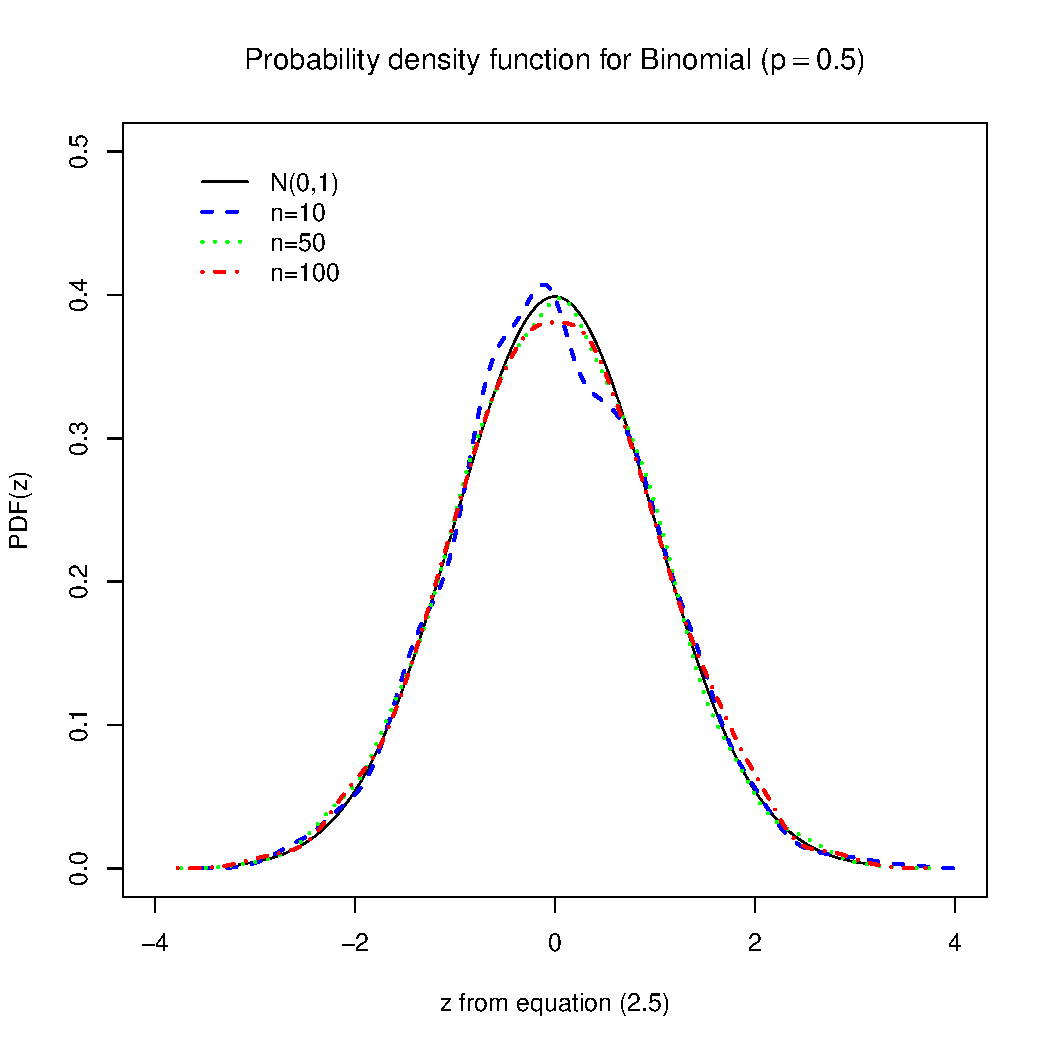
\includegraphics[width=0.49\textwidth]{Figures/binomial_PDF.pdf} \hfill
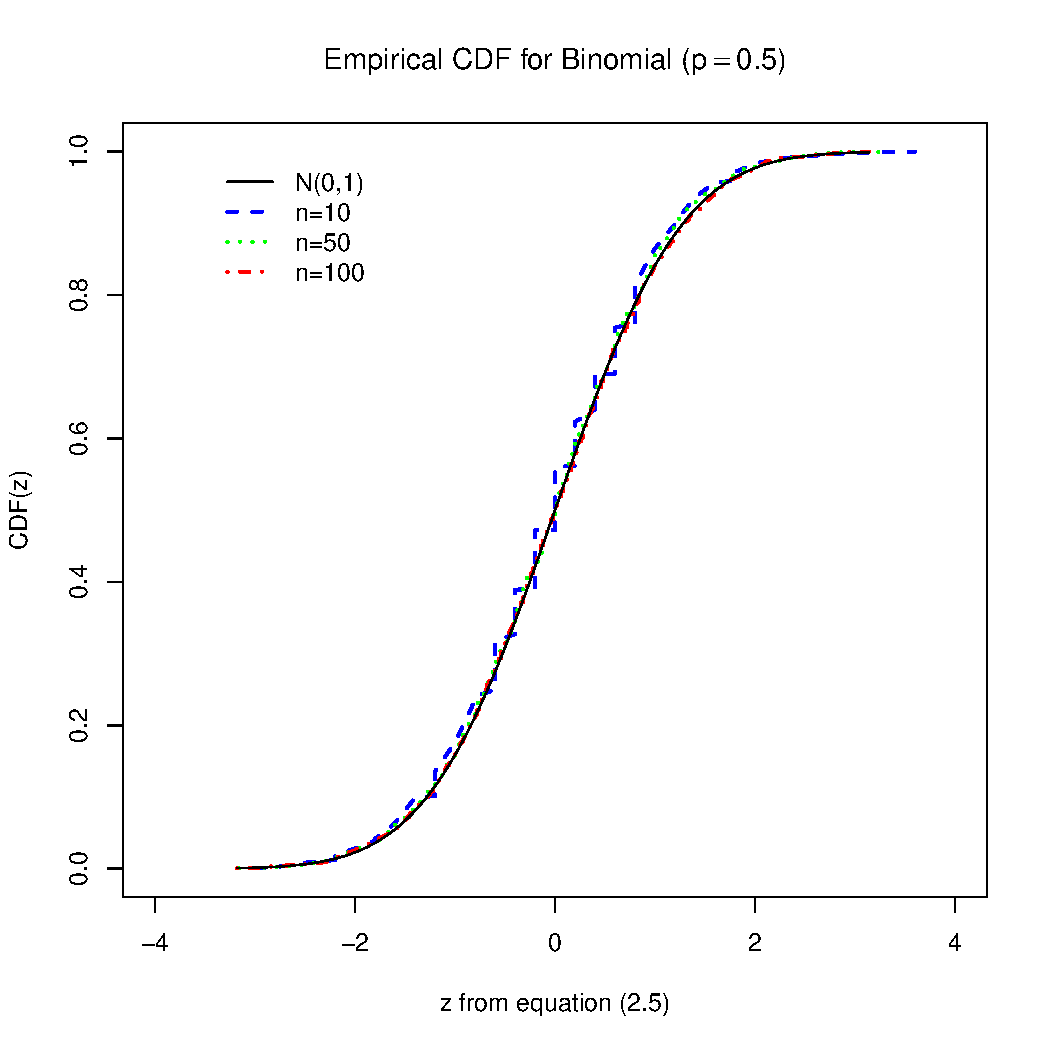
\includegraphics[width=0.49\textwidth]{Figures/binomial_CDF.pdf}\\
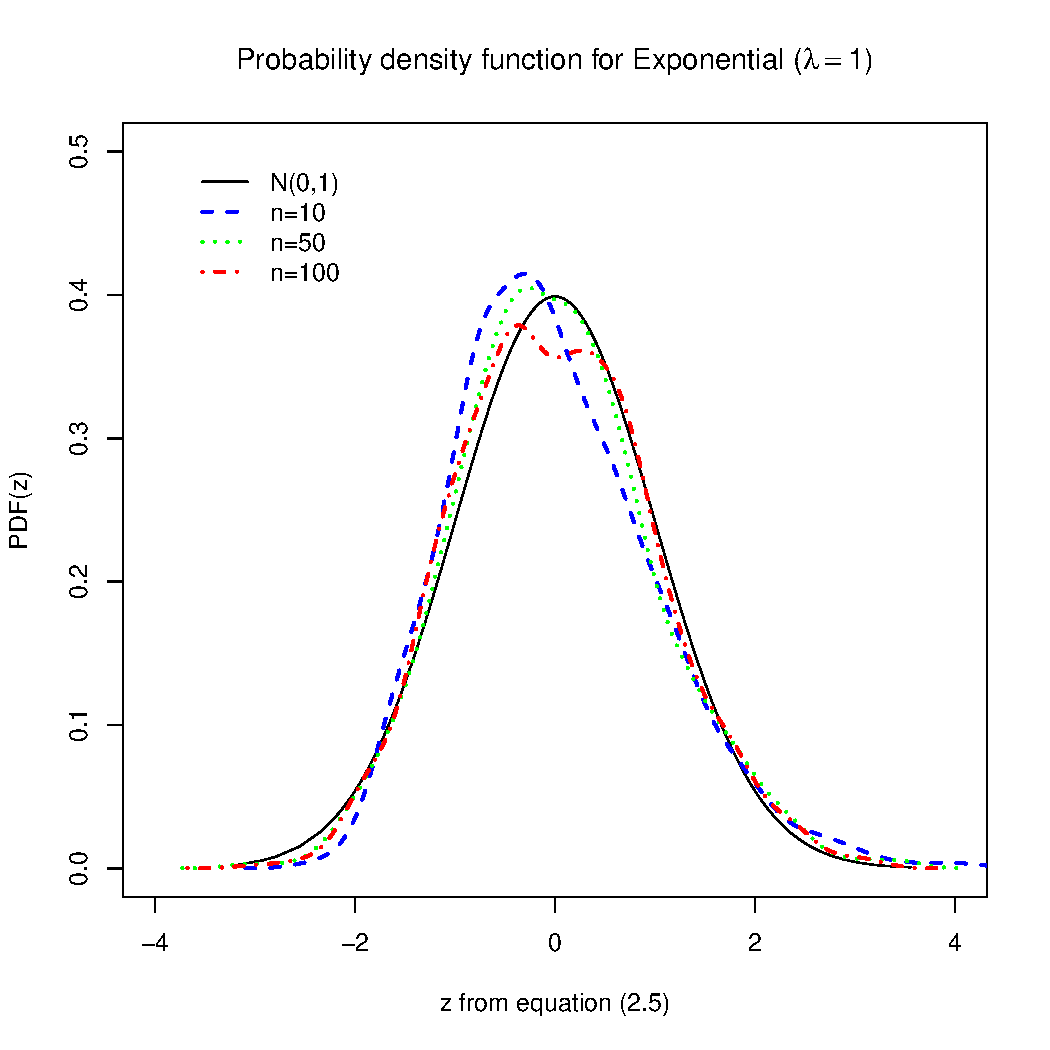
\includegraphics[width=0.49\textwidth]{Figures/expon_PDF.pdf} \hfill
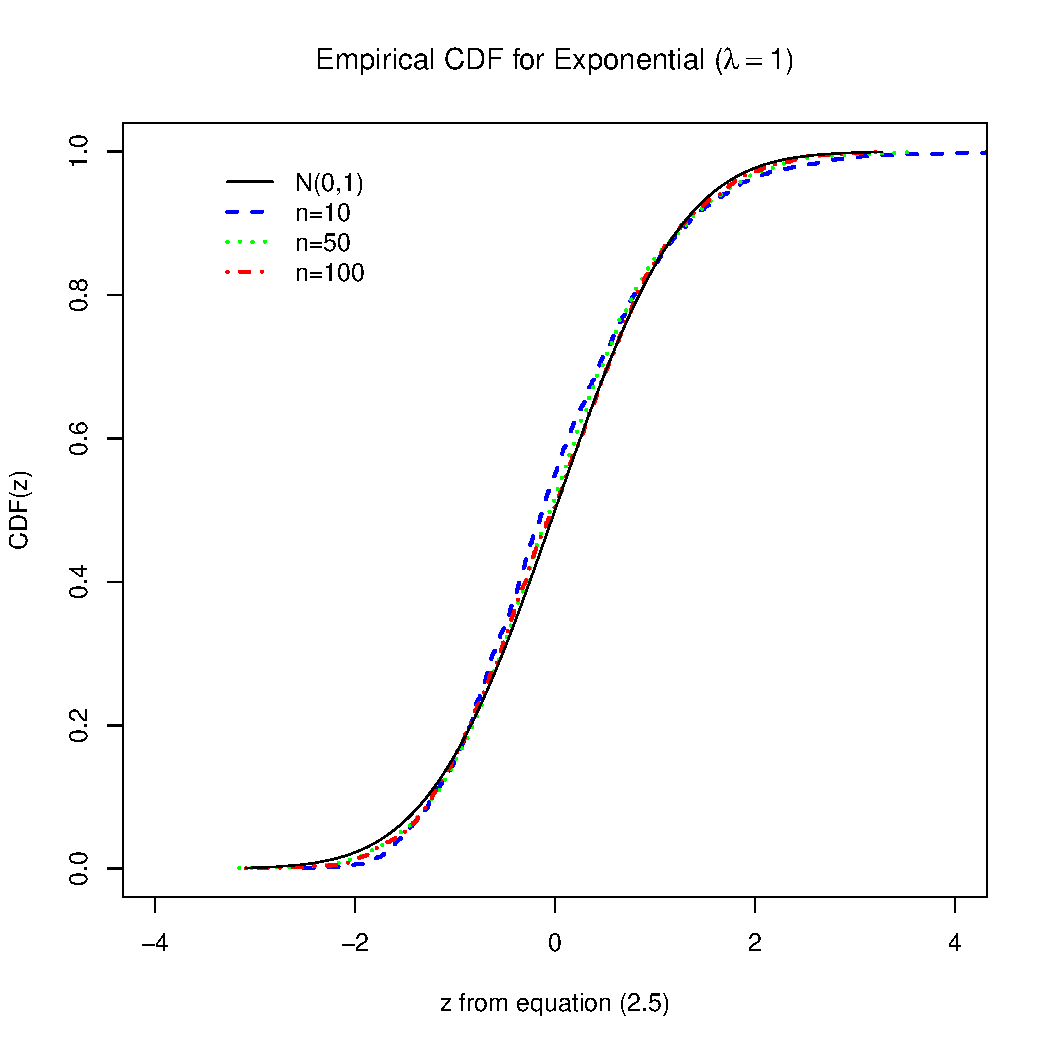
\includegraphics[width=0.49\textwidth]{Figures/expon_CDF.pdf}\\
\caption{Normal approximation for binomial and exponential distribution}\label{fig.CLT1}
\end{figure}

\begin{figure}[htp]
\centering
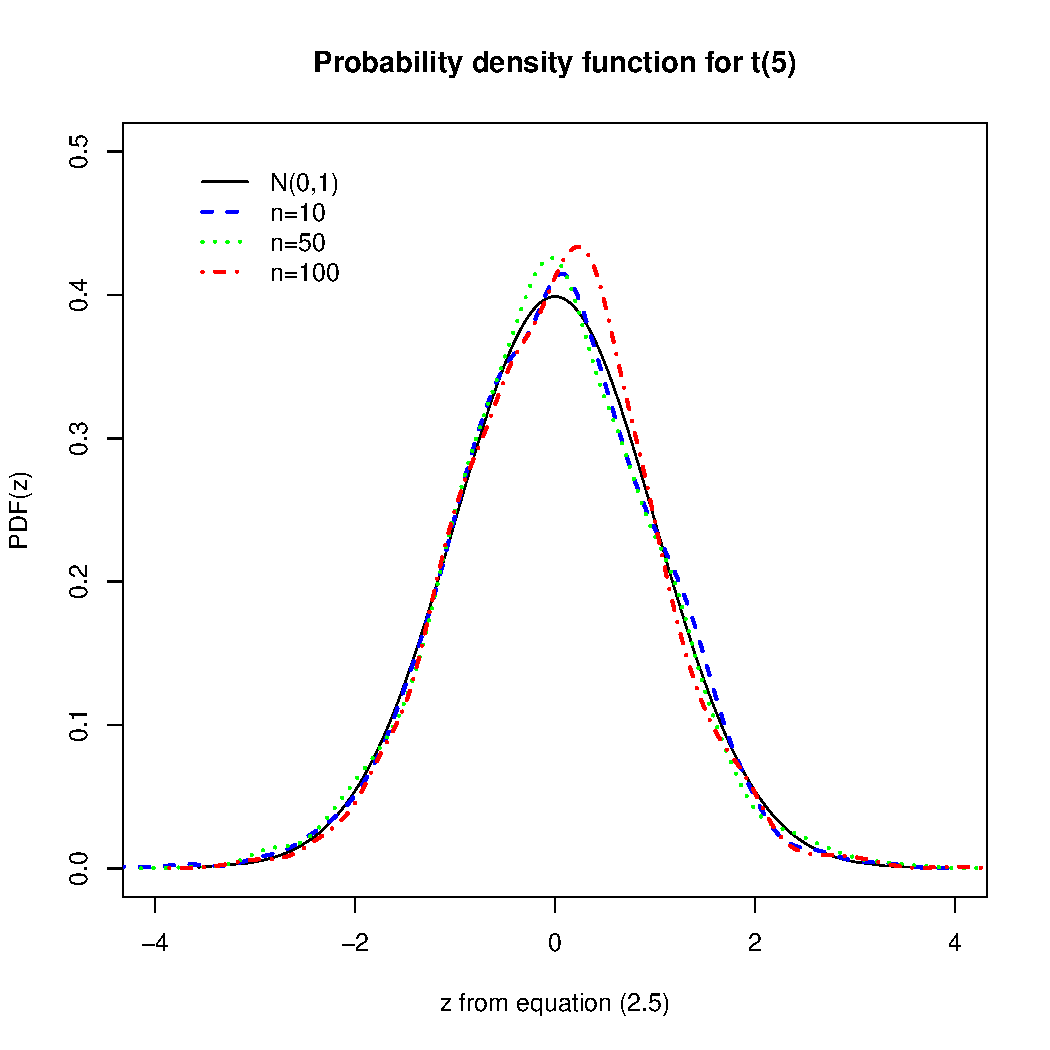
\includegraphics[width=0.49\textwidth]{Figures/t_PDF.pdf} \hfill
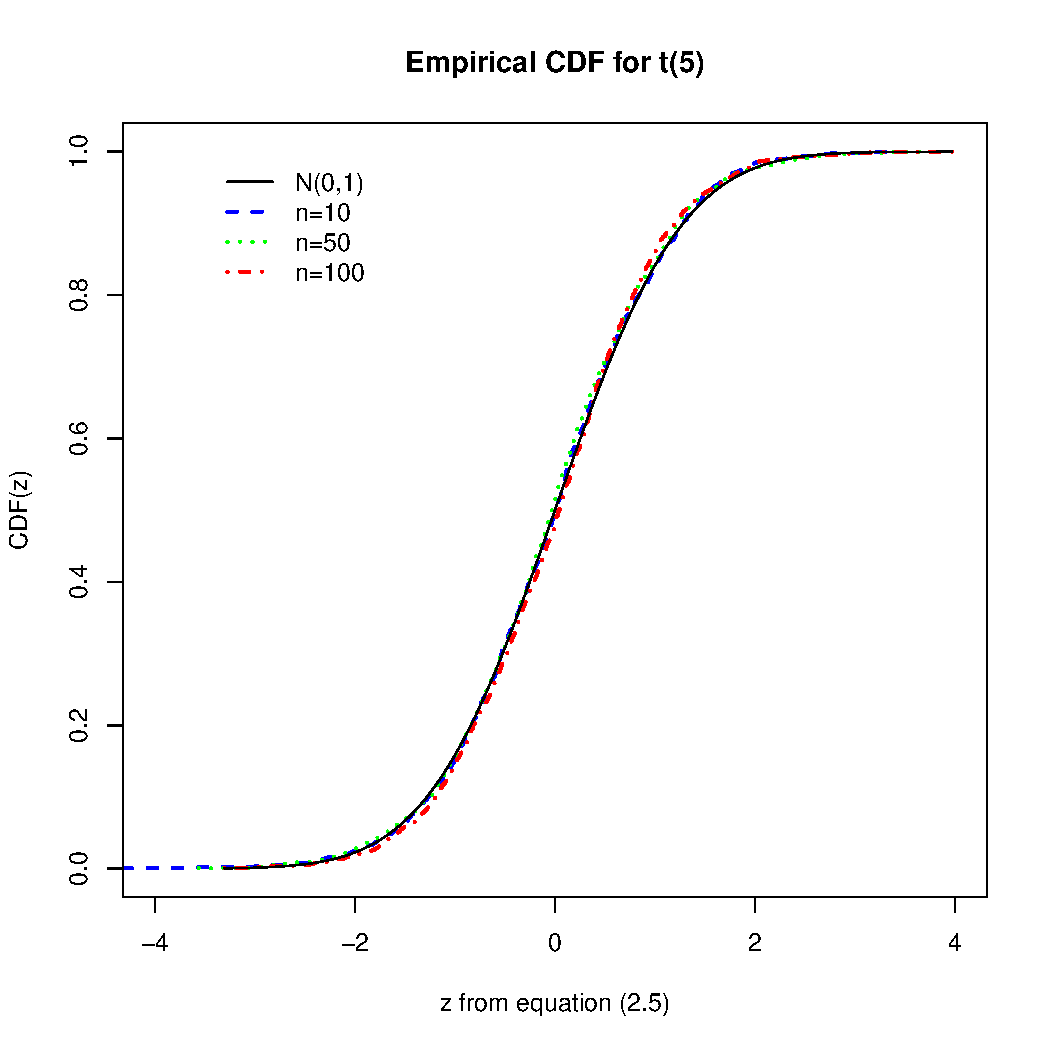
\includegraphics[width=0.49\textwidth]{Figures/t_CDF.pdf}\\
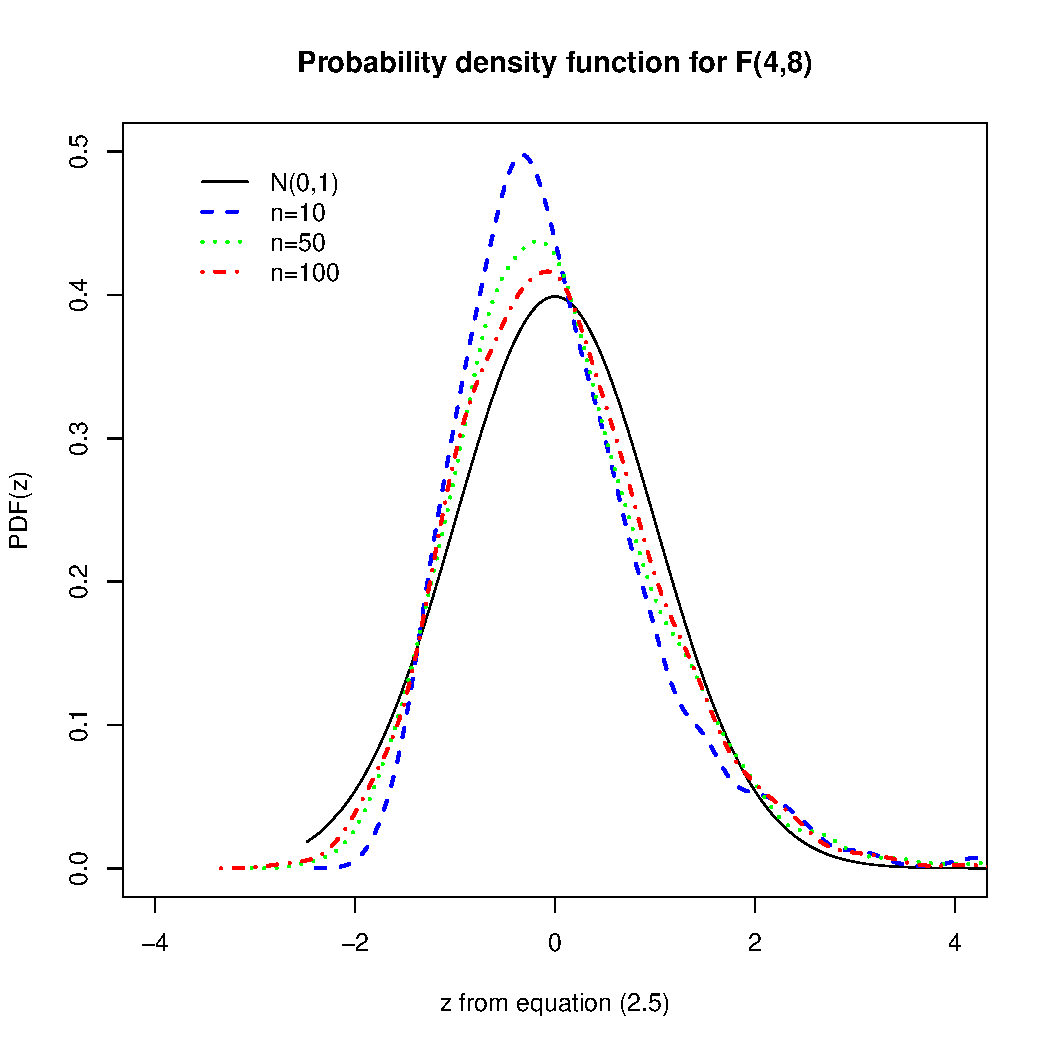
\includegraphics[width=0.49\textwidth]{Figures/f_PDF.pdf} \hfill
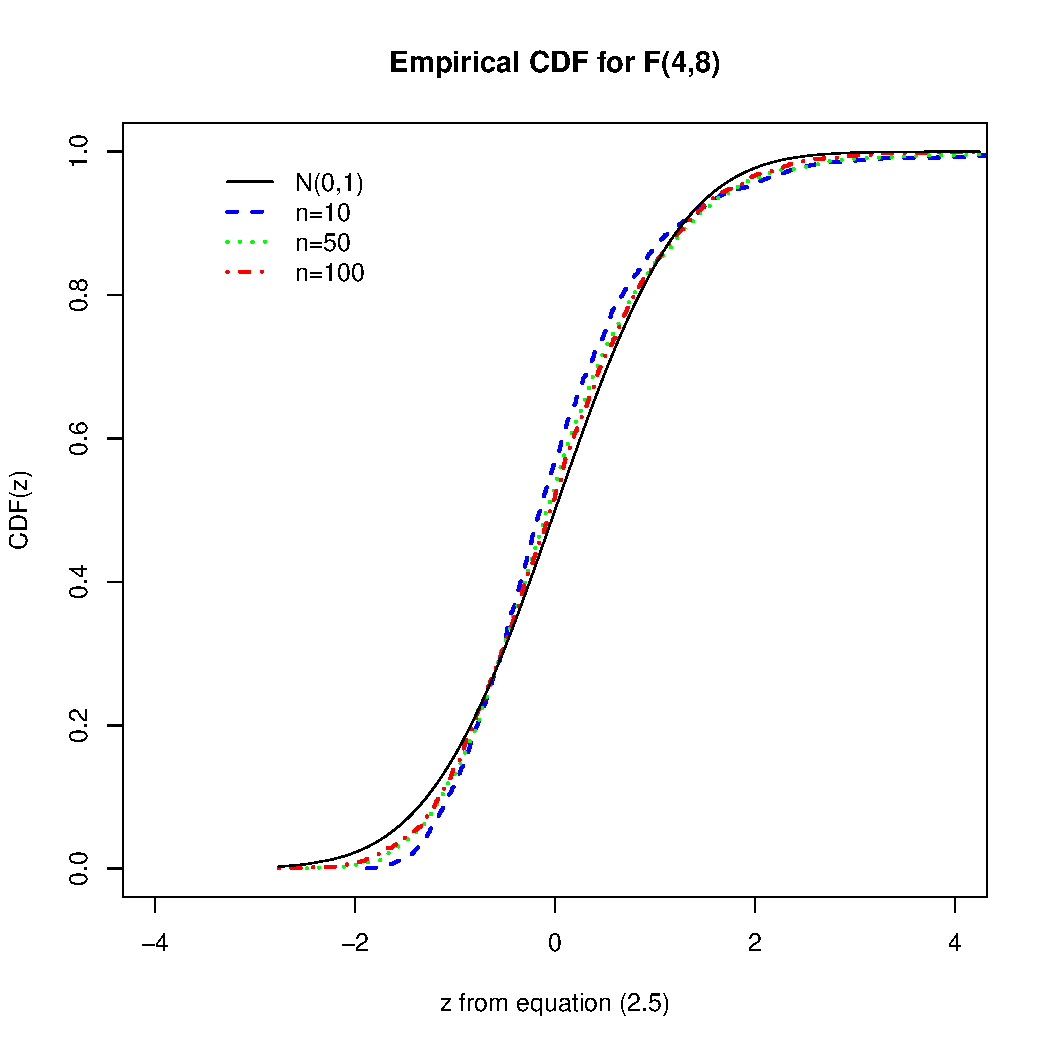
\includegraphics[width=0.49\textwidth]{Figures/f_CDF.pdf}\\
\caption{Normal approximation for $t$- and $F$-distribution}\label{fig.CLT2}
\end{figure}

\begin{figure}[htp]
\centering
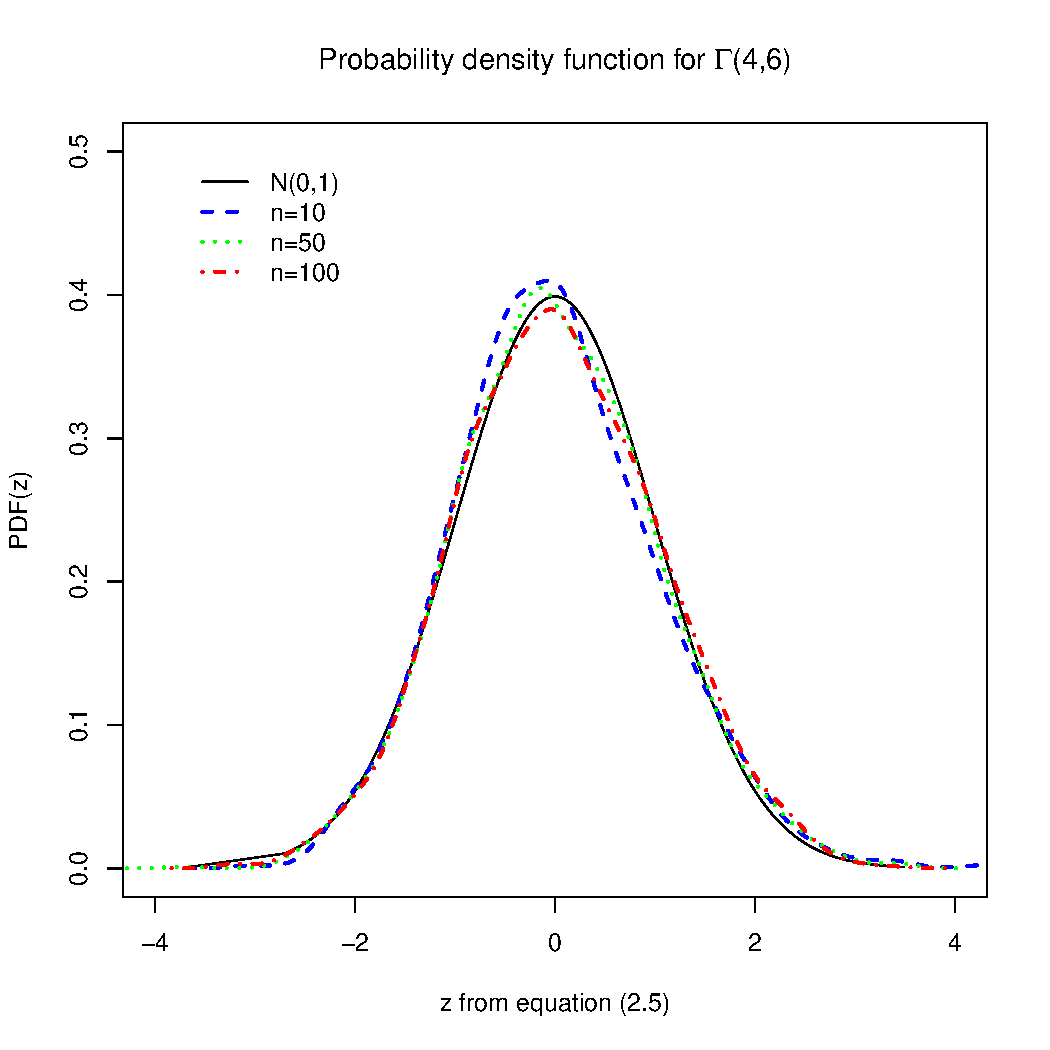
\includegraphics[width=0.49\textwidth]{Figures/gamma_PDF.pdf} \hfill
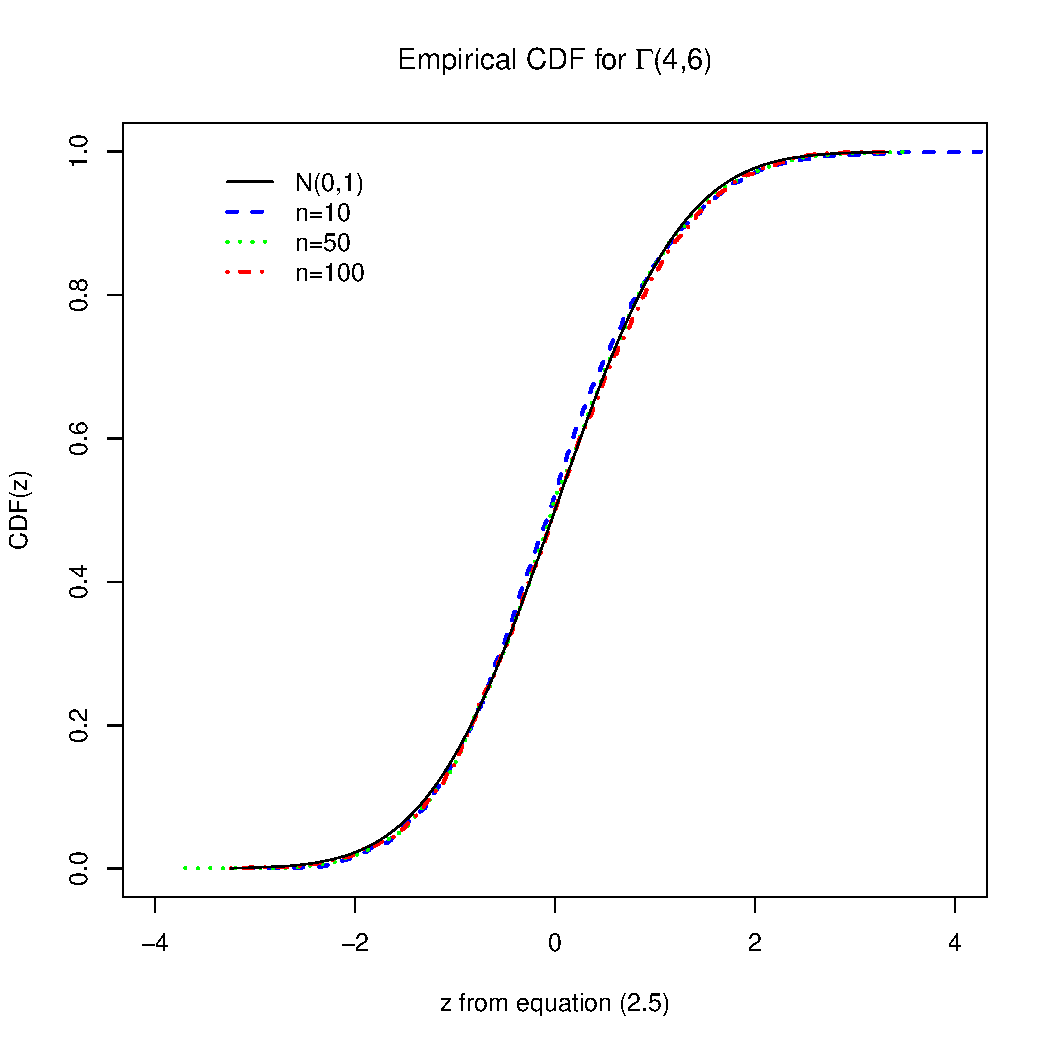
\includegraphics[width=0.49\textwidth]{Figures/gamma_CDF.pdf}\\
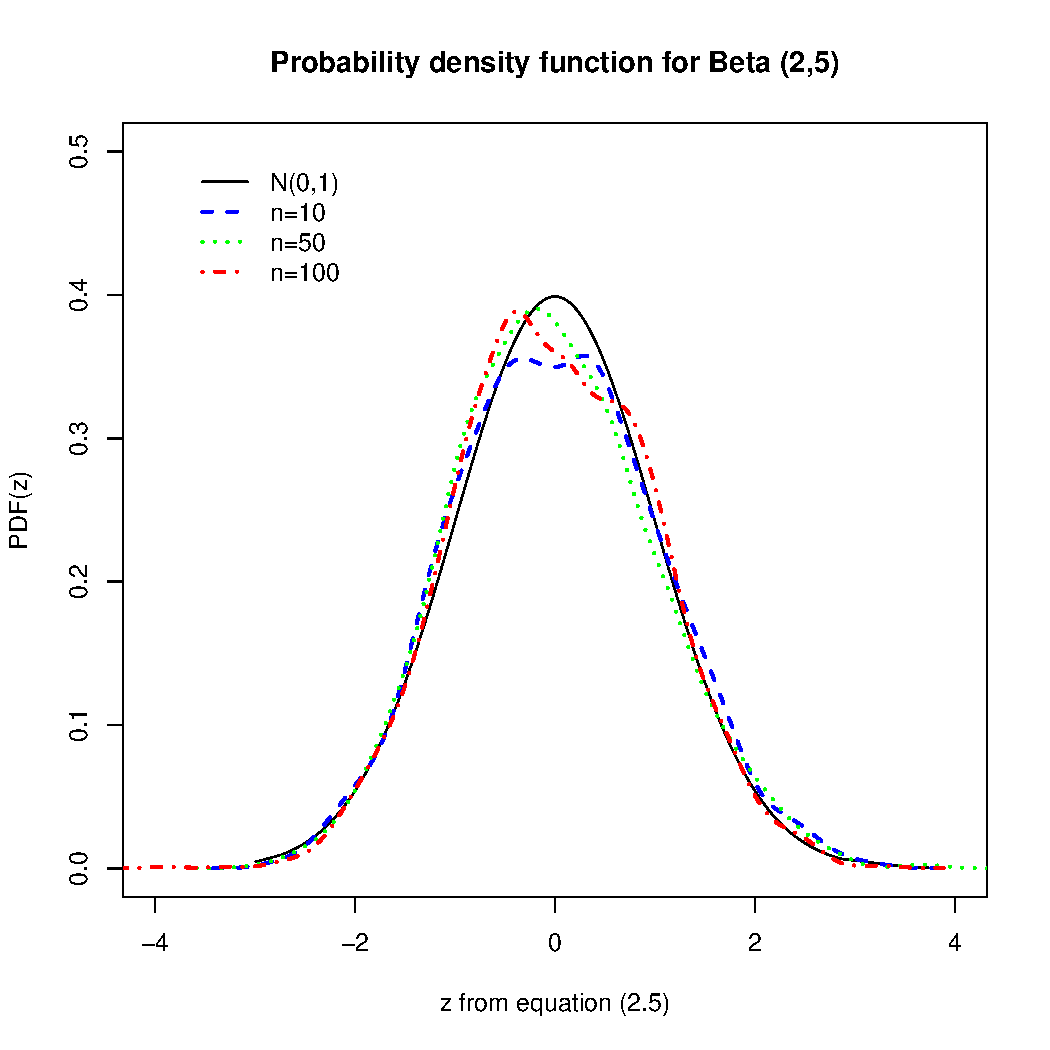
\includegraphics[width=0.49\textwidth]{Figures/beta_PDF.pdf} \hfill
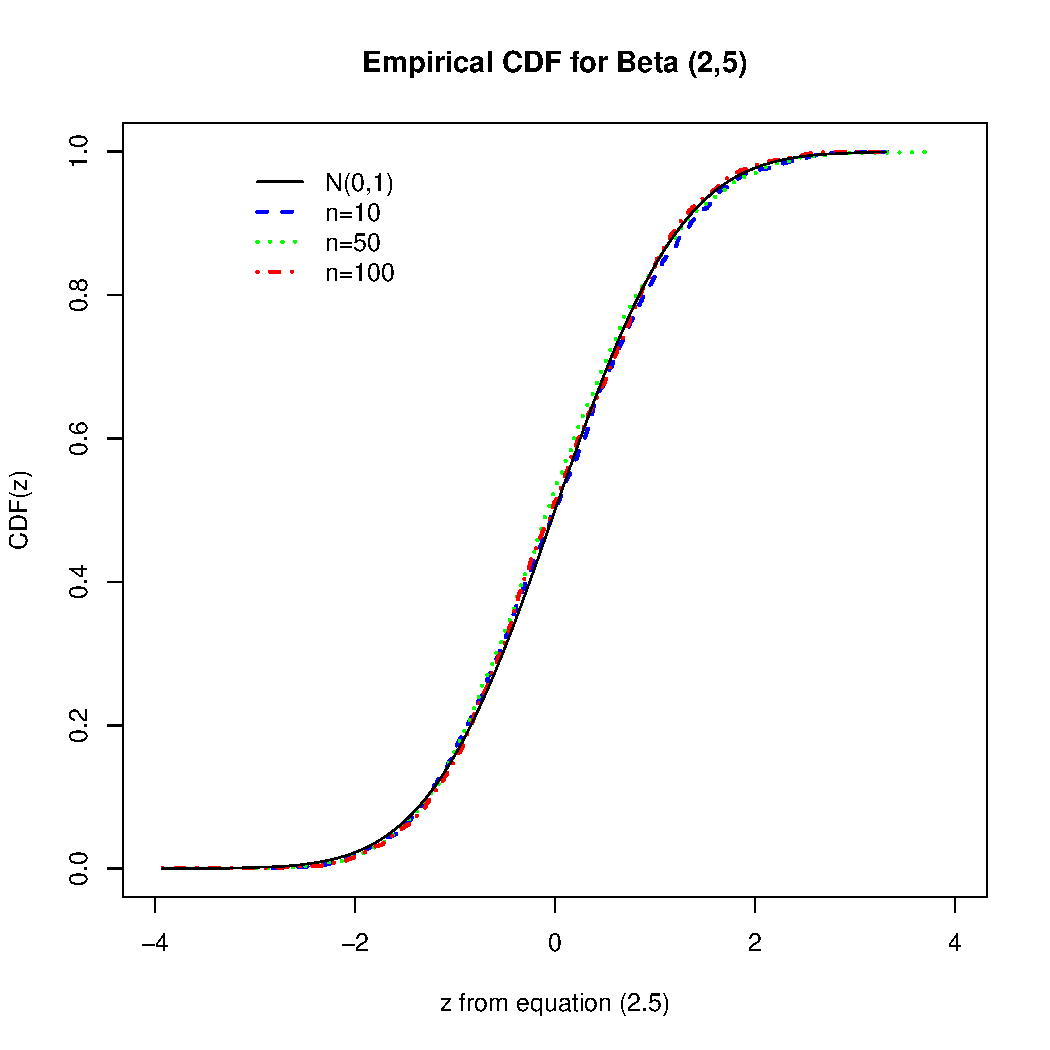
\includegraphics[width=0.49\textwidth]{Figures/beta_CDF.pdf}\\
\caption{Normal approximation for $\Gamma$- and Beta distribution}\label{fig.CLT3}
\end{figure}

Overall, this exercise demonstrates how powerful the CLT really is; for all six different distributions, $1/\sqrt(n)$ times the sum of $n$ centered random variables approximately follows a normal distribution even at $n$ as small as 10. Figures~\ref{fig.CLT1} to figure~\ref{fig.CLT3} show the empirical distribution functions for the six distributions.

\begin{itemize}
\item[\emph{Binomial}] The approximation to the standard normal distribution increases dramatically at $n=50$ as the step function is still visible at $n=10$.
\item[\emph{Exponential}] CLT takes effect visibly at $n=50$
\item[\emph{t}] Even at $n=10$, the centered random variables from the $t$-distribution approximate N(0,1) well. It is hardly surprising since the two distributions are very similar except that the t-distribution displays wider tails.
\item[\emph{F}] Centering for random variables from the $F$-distribution approximates the normal distribution only at comparatively large $n$, with the CLT fully taking effect at $n=100$
\item[\emph{Gamma}] Centered random variables from the $\Gamma$-distribution approximate N(0,1) reasonably well at the smallest $n$ with the CLT kicking more reliably at $n=50$.
\item[\emph{Beta}] Even at $n=10$, the centered random variables from the Beta-distribution approximate N(0,1) well. However for this distribution, the CLT-threshold seems to depend significantly on the random seed and fluctuated in different simulations between $n=10$ and $n=50$.
\end{itemize}

In addition to discovering that the CLT becomes effective at relatively small $n$ for a variety of distributions, this exercise demonstrates the impact of the variance on the centering process. The $\chi^{2}(m)$ distribution approaches the N($m,2m$) as $m$ becomes large and its variance is $2m$.

\begin{figure}[htp]
\centering
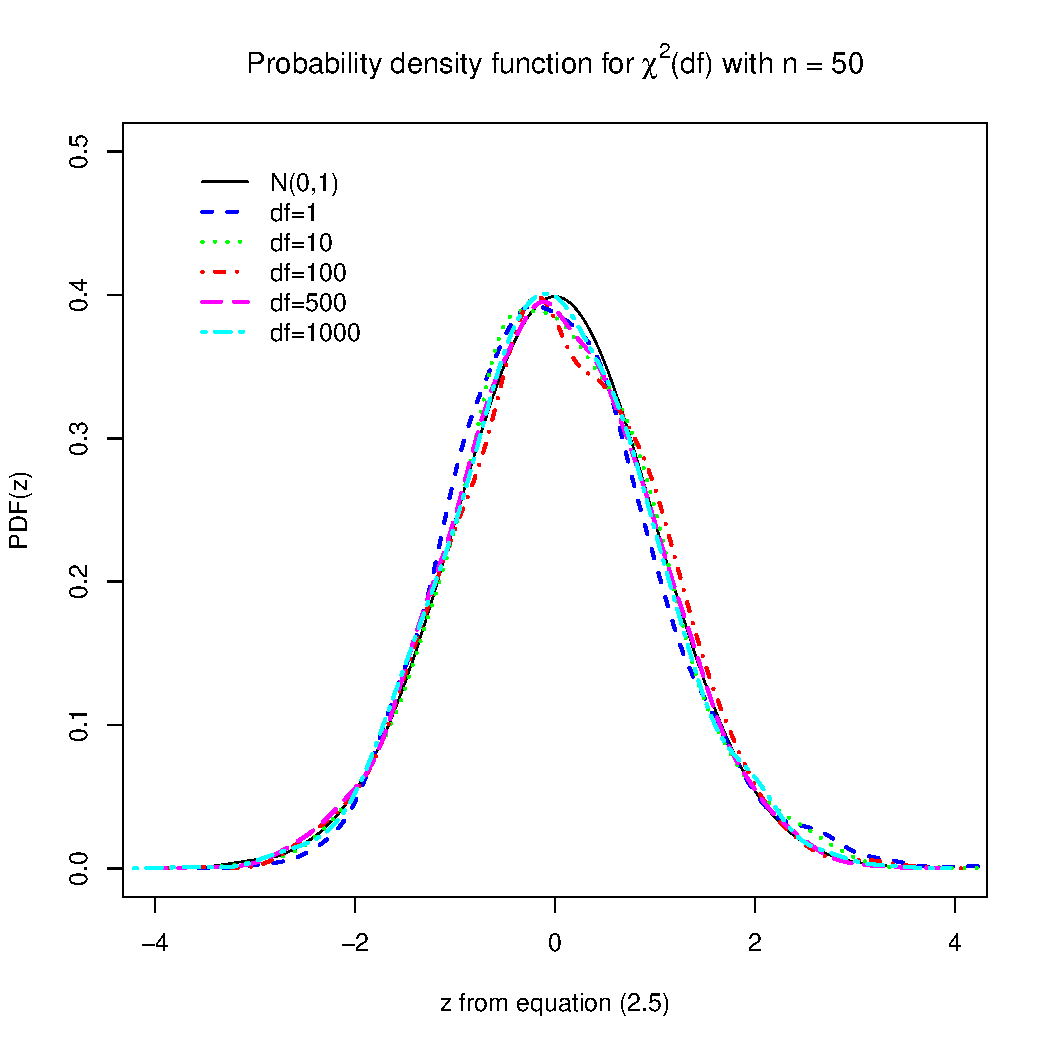
\includegraphics[width=0.75\textwidth]{Figures/chi1_PDF.pdf}
\caption{Normal approximation for $\chi^{2}$-distribution}\label{fig.CLT5}
\end{figure}

The different panels of figure~\ref{fig.CLT6} demonstrate that the \emph{variance} and \emph{sample size} work as \emph{substitutes} in the centering process; a higher variance requires a smaller sample size in order for the $\chi^{2}(m)$-distribution to approximate the standard normal distribution. This largely due to the fact that centering is achieved by subtracting the mean and dividing by the standard deviation. A large variance implies a large denominator which in turn implies that a smaller number of observations are required for the distribution to be asymptotically distributed as N(0,1).

\begin{figure}[htp]
\centering
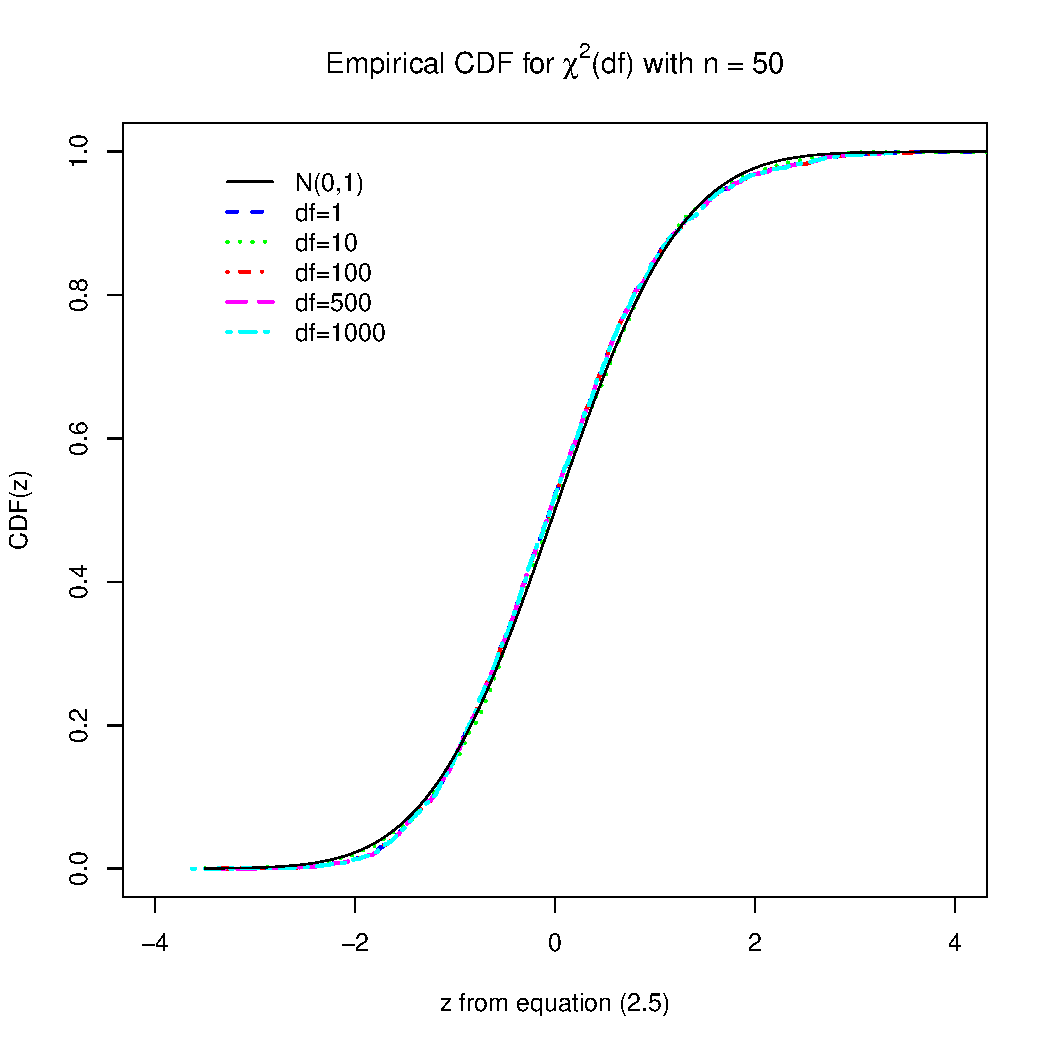
\includegraphics[width=0.49\textwidth]{Figures/chi2_CDF.pdf} \hfill
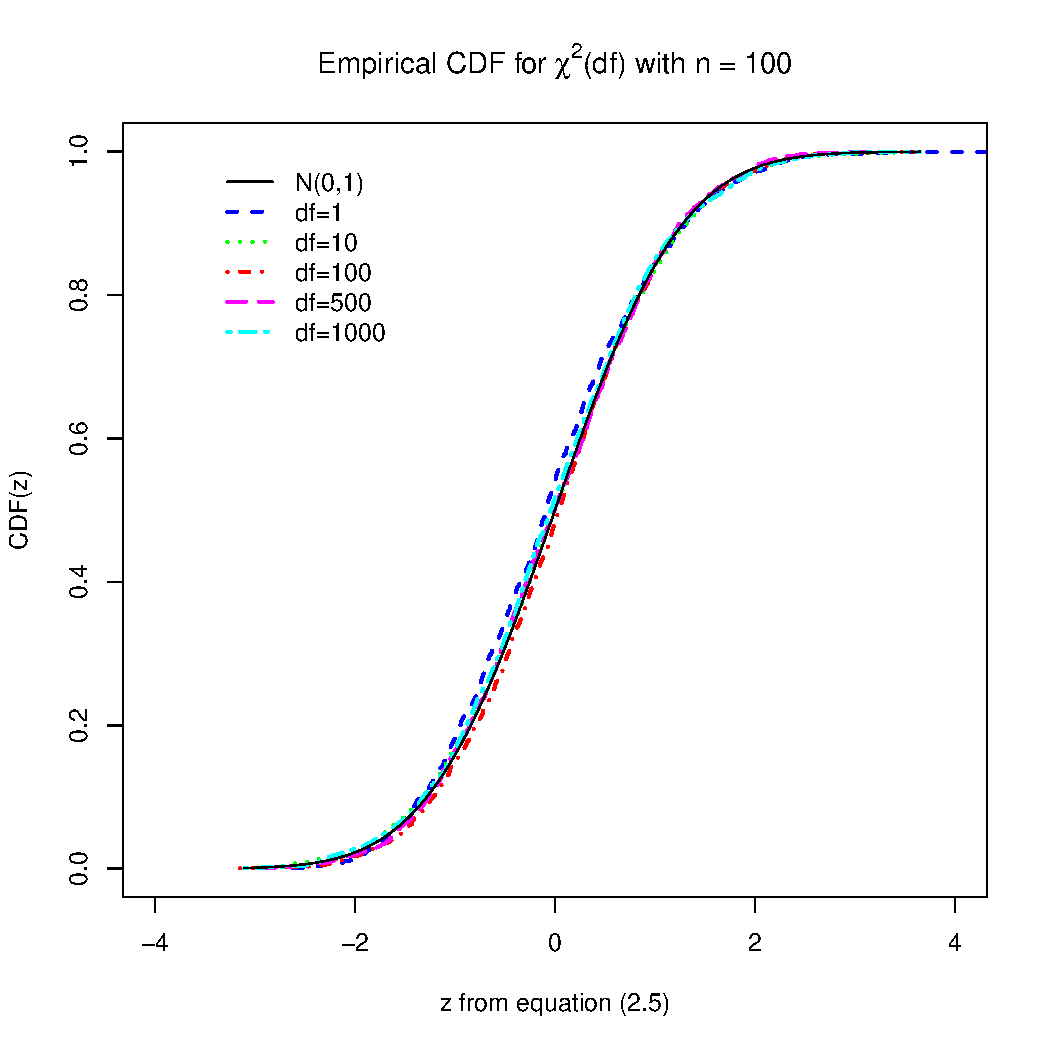
\includegraphics[width=0.49\textwidth]{Figures/chi3_CDF.pdf}\\
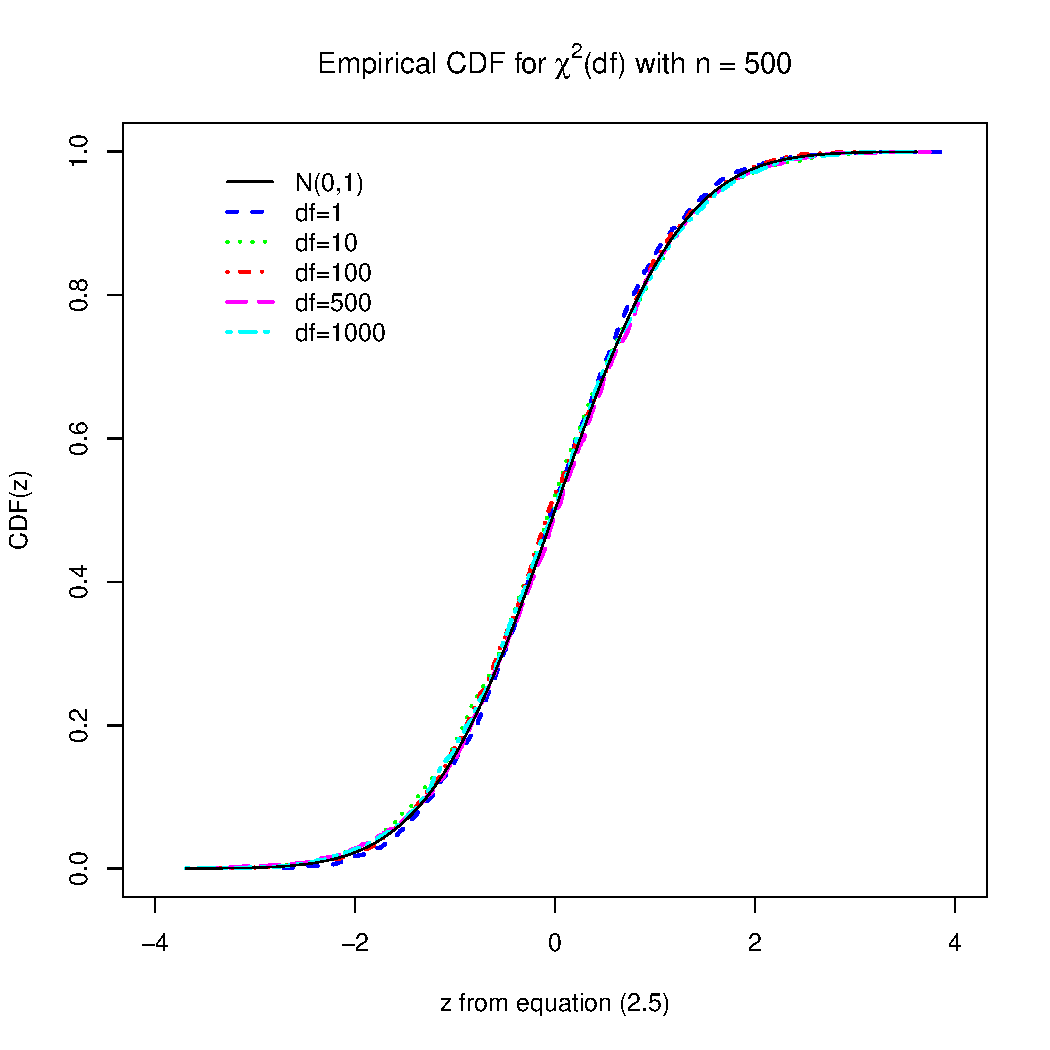
\includegraphics[width=0.49\textwidth]{Figures/chi4_CDF.pdf} \hfill
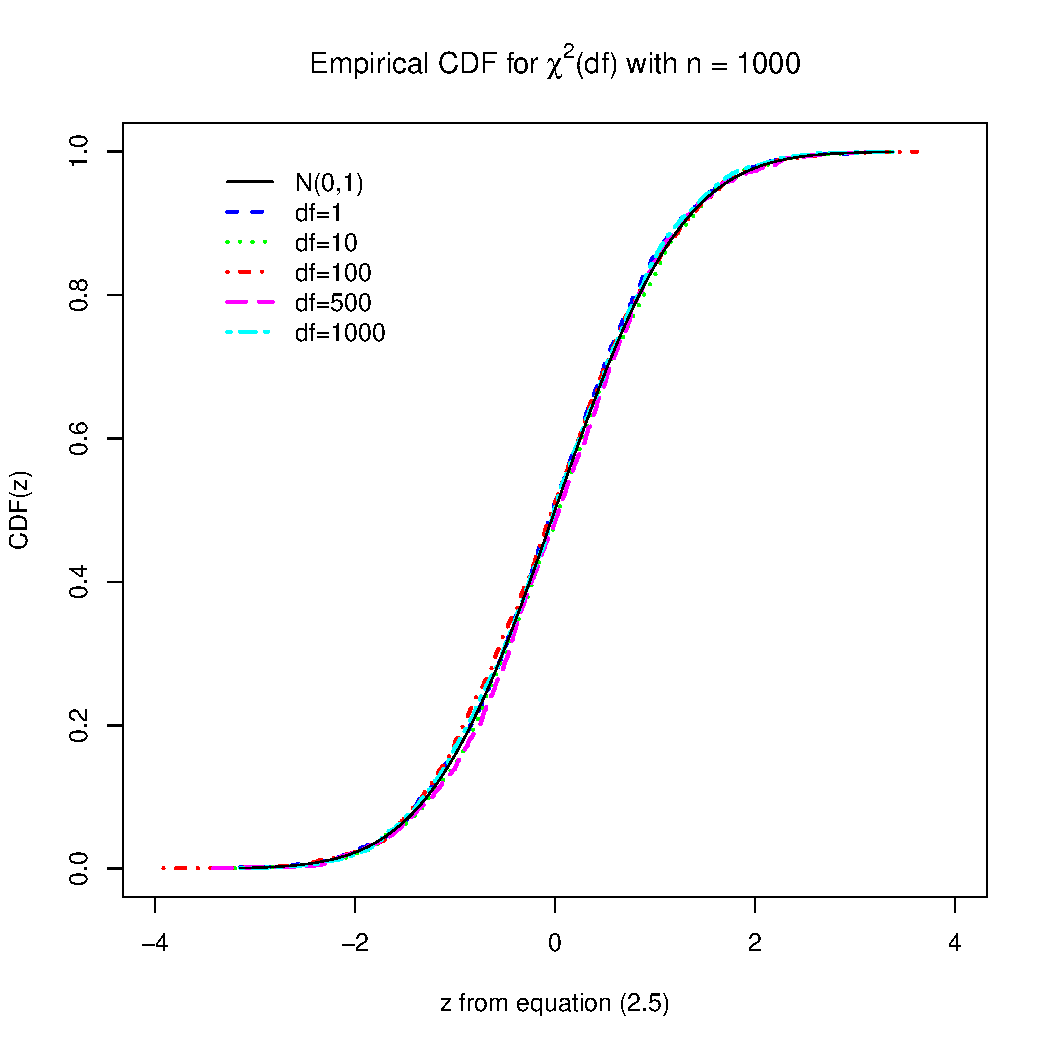
\includegraphics[width=0.49\textwidth]{Figures/chi5_CDF.pdf}\\
\caption{Variance impact and CLT for $\chi^{2}$-distribution}\label{fig.CLT6}
\end{figure}


\section{Matrix algebra}\label{chap_Review:Matrix}

\renewcommand\bibname{Further reading}
\begin{subappendices}
\bibliographystyle{econometrica}
\bibliography{Literature/OverLord}
\IfFileExists{Literature/Review.bbl}{\input{Literature/Review.bbl}}{\typeout{Need to run bibtex}}
\end{subappendices} }{\typeout{Need to run bibtex}}
\end{subappendices} }{\typeout{Need to run bibtex}}
\end{subappendices} }{\typeout{Need to run bibtex on Review}}
\end{subappendices}
